%%
%% Automatically generated file from DocOnce source
%% (https://github.com/hplgit/doconce/)
%%


%-------------------- begin preamble ----------------------

\documentclass[%
twoside,                 % oneside: electronic viewing, twoside: printing
final,                   % or draft (marks overfull hboxes, figures with paths)
chapterprefix=true,      % "Chapter" word at beginning of each chapter
open=right               % start new chapters on odd-numbered pages
10pt]{book}

\listfiles               % print all files needed to compile this document

\usepackage{relsize,epsfig,makeidx,color,setspace,amsmath,amsfonts}
\usepackage[table]{xcolor}
\usepackage{bm,microtype}

\usepackage{fancyvrb} % packages needed for verbatim environments


\usepackage[T1]{fontenc}
%\usepackage[latin1]{inputenc}
\usepackage[utf8]{inputenc}

\usepackage{lmodern}         % Latin Modern fonts derived from Computer Modern

% Hyperlinks in PDF:
\definecolor{linkcolor}{rgb}{0,0,0.4}
\usepackage[%
    colorlinks=true,
    linkcolor=linkcolor,
    urlcolor=linkcolor,
    citecolor=black,
    filecolor=black,
    %filecolor=blue,
    pdfmenubar=true,
    pdftoolbar=true,
    bookmarksdepth=3   % Uncomment (and tweak) for PDF bookmarks with more levels than the TOC
            ]{hyperref}
%\hyperbaseurl{}   % hyperlinks are relative to this root

\setcounter{tocdepth}{2}  % number chapter, section, subsection

% Tricks for having figures close to where they are defined:
% 1. define less restrictive rules for where to put figures
\setcounter{topnumber}{2}
\setcounter{bottomnumber}{2}
\setcounter{totalnumber}{4}
\renewcommand{\topfraction}{0.85}
\renewcommand{\bottomfraction}{0.85}
\renewcommand{\textfraction}{0.15}
\renewcommand{\floatpagefraction}{0.7}
% 2. ensure all figures are flushed before next section
\usepackage[section]{placeins}
% 3. enable begin{figure}[H] (often leads to ugly pagebreaks)
%\usepackage{float}\restylefloat{figure}

% prevent orhpans and widows
\clubpenalty = 10000
\widowpenalty = 10000

% Make sure blank even-numbered pages before new chapters are
% totally blank with no header
\newcommand{\clearemptydoublepage}{\clearpage{\pagestyle{empty}\cleardoublepage}}
%\let\cleardoublepage\clearemptydoublepage % caused error in the toc

% --- end of standard preamble for documents ---


% insert custom LaTeX commands...

\raggedbottom
\makeindex

%-------------------- end preamble ----------------------

\begin{document}



% ------------------- main content ----------------------

%\documentclass[11pt, a4paper]{scrartcl}
%\usepackage{graphicx}
%\begin{document}
%\changepage{0pt}{0pt}{0pt}{0.375in}{0pt}{0.4in}{0pt}{0pt}{0pt}
\thispagestyle{empty}
\begin{center}        % Sentrerer teksten
  %Tittel
  \vspace{5mm}          % Vertikalt mellomrom
  \LARGE
  %\textbf{Non-Newtonian effects on cerebral \\aneurysms using sex specific data} \\
  %\textbf{SIMULATION OF NON-NEWTONIAN BLOOD \\FLOW EFFECTS ON CEREBRAL ANEURYSMS \\USING SEX SPECIFIC DATA} \\
  %\textbf{SENSITIVITY ANALYSIS OF SIMULATED \\BLOOD FLOW IN CEREBRAL ANEURYSMS} \\
  \textbf{Mathematical analysis of epidemic systems \\ comparison of different models}
  \Large
  \vspace{5mm}
  \textbf{by} \\
  \vspace{5mm}
  %Forfatter
  \large
  \textbf{TORBJØRN PASCHEN SELAND} \\
  %Avdeling for mekanikk
  \vspace{30mm}
  \Large
  {\bf{\textsl{THESIS}}} \\
  \textsl{for the degree of} \\
  \vspace{2mm}
  %%%%%%%OLD%%%%%%{\bf{\textsl{CANDIDATUS SCIENTIARUM}}} \\
  {\bf{\textsl{MASTER OF SCIENCE}}} \\
  \vspace{5mm}
  {\large \textsl {(Master i Anvendt matematikk og mekanikk)}}\\
  \vspace{10mm}
  \centerline{
\includegraphics[width=4cm,height=4cm]{uiologo.png}}
  \vspace{5mm}
  % \textsl{Mechanics Division, Department of Mathematics} \\
  \textsl{Faculty of Mathematics and Natural Sciences} \\
  \textsl{University of Oslo} \\
  %Maaned, aar
  \vspace{10mm}
  \large
  \textsl{December 2014} \\
  \vspace{5mm}
  \normalsize
  % \textsl{Avdeling for mekanikk, Matematisk institutt} \\
  \textsl{Det matematisk- naturvitenskapelige fakultet} \\
  \textsl{Universitetet i Oslo} \\
\end{center}
%\end{document}



\newcommand{\Imax}{I_{\textrm{max}}}

\chapter*{Abstract}
This thesis study and compare three different models for modeling epidemic diseases. The simulations are done for a small group over a short time period. In the first chapter an ODE model is presented. This is used to model two different examples of epidemic systems. The second chapter introduce a PDE model, which also takes the position into account. The parameters from the first model is used for the PDE model, to study the spatial effect. Random walk is used as the third model. Here, human behavior has been added to the model to achieve a more realistic result. Throughout the thesis two examples are used, namely a influenza outbreak in an English boarding school and a potential zombiefication based on the TV series \emph{Walking Dead}. The results from these two cases are used to compare the different models. 

\chapter*{Acknowledgements}
First, I would like to thank my supervisors Kent-Andre Mardal and Hans Petter Langtangen for their guidance and knowledge. A special thanks to Kent-Andre for the good discussions about humans ability to survive a zombie attack.


\vspace{3mm}


I would also like to thank my fellow students in B1002 for their company and good support. A special thanks to Ada and Aslak for reading my thesis, and for constructive feedback. Thanks to my sister-in-law,Trine, who has done an amazing job helping me with my English.


\vspace{3mm}


Finally, I would like to thank my two favorite girls, my daughter Tiril and my wife Silje. Thank you for supporting me with constant love and comfort.     



\tableofcontents


\vspace{1cm} % after toc





\chapter{Introduction}
Throughout history large epidemic diseases have spread around the world, often over large geographical areas. These diseases have done great harm on the population and millions of people have died. The Black Death and Cholera are epidemics that have moved over large distances into Europe. When the Black Death came to Europe in 1347, it killed about a third of the population, which at that time was about 85 million people Ref.\cite[p.~315]{murray2002mathematical}.~These diseases often gave physical symptoms, which have given important knowledge through history to prevent new outbursts and to cure already infected humans. They have various outbreaks, but are often related to connections between humans and animals. Malaria is an example of a disease that transmits from mosquitoes to humans. There have also been various explanations of the spread and cause of epidemics. AIDS(autoimmune deficiency syndrome) has as an example been ascribed by many as a punishment sent by God. Ref.\cite[p.~316]{murray2002mathematical}.~


\vspace{3mm}




\vspace{3mm}


The first major epidemic in the U.S.A was the Yellow Fever, discovered in 1793 in Philadelphia. 5000 of a population of 50 000 died. About 20 000 fled the city and the situation was quite chaotic Ref.\cite[p.~316]{murray2002mathematical}.~This had a major impact on the subsequent life and politics of the country. The power of a disease can do larger damage, with respect to death, than a war.


\vspace{3mm}




\vspace{3mm}


After World War II, public health strategy has focused on elimination and control of organisms which cause disease. In 1978 United Nations sat a goal of eradicating all diseases by year 2000. A large job has been done and smallpox is an example of a disease that was last seen in Somalia in 1977[Ref:cdc.gov]. AIDS was later recognized and has been difficult to stop the spread.


\vspace{3mm}




\vspace{3mm}


Another important aspect in the current spread of diseases, is the displacement of human populations. About a million people cross international borders daily. The growth of human population, especially in underdeveloped countries, is a factor that affects the spread. These conditions played a key role in the spread of HIV(human immunodeficiency) in the 1980's. World Health Organization has estimated that around 32.6 million are infected with the HIV virus today[web:http://www.who.int/features/factfiles/hiv/en/].


\vspace{3mm}




\vspace{3mm}


Knowledge through history is important for the control of different epidemics, but also important in detecting new diseases. The plague of Athens had been studied in great detail by Thucydides in 430-438 BC. Similar had been done with the 'sweating sickness' in the late 15th and first of the 16th centuries in England. The symptoms of 'sweating sickness' was detected in 1993 in the Southwest U.S.A. Here the disease was called hanta virus. There is likely that this is the same disease, but that the 'sweating sickness' has been dormant for couple of hundred years. Ref.\cite[p.~317]{murray2002mathematical}.~


\vspace{3mm}




\vspace{3mm}


There have been done several mathematical studies on different diseases. HIV/AIDS is a field which has been studied by several scientists through the years. \emph{Mathematical Modelling of the Transmission Dynamics of HIV Infection and AIDS: a Review} was published in 1988 by Valerie Isham Ref.\cite{isham1988mathematical}. This paper focuses on modelling transmission of infection in the context of AIDS epidemic.In 1999 Alan S. Perelson and Patrick W. Nelson published \emph{Mathematical Analysis of HIV-1 Dynamics in Vivo} Ref.\cite{perelson1999mathematical}. They studied the dynamics of HIV-1 pathogenesis to AIDS, where they looked at rapid dynamical processes that occur in short time scales, as hours, while AIDS occurs on a time scale of about 10 years. This affect the way that AIDS patients are treated with drugs. \emph{Predicting the HIV/AIDS epidemic and measuring the effect of mobility in mainland China} by Xiao et. al Ref.\cite{xiao2013predicting} is another study done on HIV/AIDS where they look at the geographic variation in the severity of the epidemic in China. 


\vspace{3mm}




\vspace{3mm}


This thesis will study three mathematical models used to simulate epidemic diseases. The first chapter will use an ODE system to model the different groups that consists in an epidemic disease. The chapter will study the variations in each group based on the time aspect. The second chapter will look at a PDE system. This model also takes the spatial spread into account, and the position affects the result. A random walk system is studied in the third chapter. In the two first chapters, the amount in each group has been seen as concentrations. In this chapter, each person will be model as a particle. The person behavior will be based on the group it belongs to and the time and position of the person. 


\vspace{3mm}




\vspace{3mm}


The TV series \emph{Walking Dead} has through several seasons shown the result of a zombie outburst. A couple of studies have been done on epidemic disease, where papers from Munz et. al Ref.\cite{munz2009zombies} and Langtangen,Mardal {\&} Røtnes Ref.\cite{zombie-math} can be mentioned. This thesis will use these papers and develop the models further. It will focus on the first five episodes in the first season of \emph{Walking Dead} Ref.\cite{walking_dead}, and use parameter values based on this series. 


\vspace{3mm}




\vspace{3mm}


A couple of choices have been done for this thesis. The systems will be model for a short period of time. The longest simulations are performed for a month, while the third chapter only consists of simulations for an half hour. This is done to study the humans behavior and influence in a zombie attack. The second one is to model all systems as closed systems. The amount in each simulation never exceeds 763 humans and the time aspect is short. Therefore the birth and death rate is close to negligible, and are set to zero.    

\chapter{ODE models}
\label{section:ODE_models}
This chapter will be split into two different parts. The part includes two sections, which will be based on the chapter \emph{Dynamic of Infectious Diseases} from Mathematical Biology by J.D Murray Ref.\cite{murray2002mathematical}. \emph{Epidemic models} will give a historic perspective on different epidemic diseases and their effect on the human population. Furthermore a basic ODE system will be shown and studied to see how this model can give information about the disease. The section will check if a disease is severe for the human population, and based on this called an epidemic disease.


\vspace{3mm}




\vspace{3mm}


The last part will be based on a scenario where the population faces a zombification, one of the most critical and devastating epidemic diseases that can occur. Here, the TV series \emph{Walking Dead} will be used as reference, and the series will be tested against a model based on the SIR model explained in section \emph{Simple Epidemic models}. There have been a couple of papers on this model earlier, and this part will be based on these models and try to adjust the system to the TV series.     
\section{Simple Epidemic Models}
Most of the models shown here will have a constant population. The zombie model shown later will have a slight increase considering newborn, but this will be close to negligible. This may differ from the real world, where the population in different areas will vary with population flow. Reasons for doing this are, first of all to simplify the model and second to be able to model a closed system. How the population interacts is another assumption that has to be done. Here this is set to be similar for the whole area that is modeled. To simplify the population can be divided into three different groups. 
\begin{itemize}
\item \emph{Susceptible} ($S$), who are humans that are healthy and at risk of becoming infected. 

\item \emph{Infected} ($I$), who are humans who have the disease or are carriers of the disease. This group can infect the \emph{Susceptible}. 

\item \emph{Removed} ($R$),who are dead or recovering humans, often people that already have had the disease. 
\end{itemize}

\noindent
The natural order for a human is,
\begin{equation*}
S \rightarrow I \rightarrow R.
\end{equation*}
This model is called $SIR$ model, but the number of groups can be changed. $SI$ only consists of the two first groups and a $SEIR$ model has added an extra group \emph{Exposed} , $E$, where the disease is latent. This can be used to model the incubation time. 


\vspace{3mm}




\vspace{3mm}


The transmission of the infection and incubation period are elementary factors in the spread of a disease. These are reflected in the terms of the equations. Since this is a SIR model, the incubation time is negligible. The amount of people in each group can be seen as a function of time, expressed as $S(t),I(t)$ and $R(t)$. The growth of $I$ caused by \emph{Susceptible}, can be viewed as a rate proportional to the number of \emph{Infected} and \emph{Susceptible} multiplied by a constant,$rSI$, where $r>0$. This constant controls the efficiency of the transmission from $S$ to $I$. This will appear as a reduction in the function $S(t)$. The rate of removal from \emph{Infected} to \emph{Removed} can be viewed as the number of \emph{Infected} times a constant, $aI$, where $a>0$ controls the time spent in the \emph{Infected} group. The dynamic model will be,
\begin{equation} \label{eq:SIR_model}
	\begin{aligned} 
	\frac{dS}{dt} &= -rSI \\ 
	\frac{dI}{dt} &= rSI-aI \\ 
	\frac{dR}{dt} &= aI 
	\end{aligned}
\end{equation}
This model is called the Kermack-McKendrick(1927) model Ref.\cite[p.~320]{murray2002mathematical}.~It is considered that the groups are uniformly mixed and that there is equal probability of contact for all individuals. These assumptions will not be correct for all diseases, especially sexually transmitted diseases. The total number of the population will stay constant, since this is a closed system. This can be seen on the total change.
\begin{equation}
\frac{dS}{dt} + \frac{dI}{dt} + \frac{dR}{dt} = 0
\end{equation}

Therefore the total size of the population, $N$, will be constant. 
\begin{equation} \label{eq:SIR_N}
S(t)+I(t)+R(t) = N
\end{equation}

\section{Threshold phenomenon}
\label{section:1threshold_phenomenon}
The threshold value is essential when studying an epidemic model. To cause an epidemic situation, the model needs to fulfill $I(t)> I_0$ for some $t>0$, where $I_0$ describes the initial condition of  the \emph{Infected} group. The initial conditions can be given as,
\begin{equation} \label{eq:thres_val}
S(0)=S_0 > 0,\hspace{8mm} I(0)=I_0>0,\hspace{8mm} R(0) =0.
\end{equation}
These initial conditions given in Eq.(\ref{eq:thres_val}) combined with $r$ and $a$ controls the epidemic situation. These will affect the spread of the infection. From Eq.(\ref{eq:SIR_model}) the function for the \emph{Infected} group at initial time is,
\begin{equation}
\left[\frac{dI}{dt}\right]_{t=0} = I_0(rS_0-a)
\end{equation}
The expression inside the brackets controls the change in $I$. The function will increase if $S_0 > \frac{a}{r}$, this will therefore be the threshold value for the function. The threshold value will be described by the variable $\rho$,
\begin{equation} \label{eq:threshold_value}
\rho = \frac{a}{r}
\end{equation}
This can be shown with some phase trajectories of the \emph{Susceptible} and the \emph{Infected} in Fig.(\ref{fig:threshold_phenomenon}).  


\begin{figure}[ht]
  \centerline{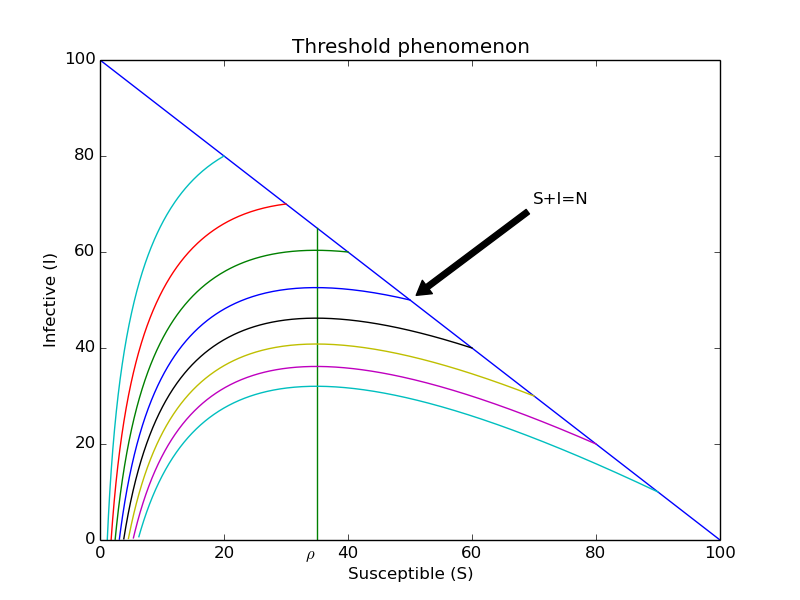
\includegraphics[width=0.8\linewidth]{1_fig/threshold_phenomenon.png}}
  \caption{
  \label{fig:threshold_phenomenon} Simulations of the SIR model (\ref{eq:SIR_model}) with start positions along the blue line. $I$ increases until $S$ is equal to the threshold value $\rho$, which is set to 35. Then $I$ is reduced to 0. In the simulations where $S_0 < \rho$, no epidemic situation is achieved.
  }
\end{figure}
%\clearpage % flush figures fig:threshold_phenomenon


The simulation shows that $I$ is based on the relation between $S$ and $\rho$. This can be described with a reproduction rate,
\begin{equation}
R_0 = \frac{rS_0}{a}
\end{equation}
It will cause an epidemic reaction if $R_0 > 1$. This parameter is crucial in the understanding of the work with the disease. To prevent a dispersion, the value of $R_0$ has to be under 1. An effective way to get control is by global vaccination programs. Smallpox is an example on a disease that nearly has been eradicated around the world. This is due to a reduction of \emph{Susceptible}. However there is always a small chance of side effects when using vaccination, and therefore some people choose to skip it. This is quite critical for the fight of total eradication. Not only is it a big risk for the specific person, but it also increases the number of \emph{Susceptible}. An epidemic situation can quickly grow again if the reproduction rate reaches the threshold.


\vspace{3mm}




\vspace{3mm}


Some analytical studies can be done on the model in Eq.(\ref{eq:SIR_model}).
\begin{equation} 
\frac{dI}{dS} = -\frac{(rS-a)I}{rSI} = -1 + \frac{\rho}{S},\hspace{8mm}\rho=\frac{a}{r}, (I\neq0).
\end{equation}
The singularities will all lie on the I=0 axis. This equation can be integrated and will then give phase plane trajectories in the (I,S) plane. This can be seen in Fig.(\ref{fig:threshold_phenomenon}).
\begin{equation} \label{eq:constant}
I+S-\rho \ln S = \textrm{constant} = I_0 + S_0 - \rho \ln S_0
\end{equation}
All initial values satisfy $I_0+S_0=N$ since $R(0) = 0$. This will change when $t>0$. If a disease appears it would be important to know the severity of the disease and the chance of developing to an epidemic disease. Therefore it is crucial to know the maximum value $\Imax$ which occurs when $S=\rho$. At this point, $\frac{dI}{dt}=0$. This can be found by using (\ref{eq:constant})
\begin{align} 
I+S-\rho \ln S =& I_0 + S_0 - \rho \ln S_0 \nonumber \\
\Imax+\rho-\rho \ln \rho =& I_0 + S_0 - \rho \ln S_0\nonumber \\
\Imax=&- \rho+\rho \ln \rho + I_0 + S_0 - \rho \ln S_0\nonumber \\
\Imax=&N - \rho + \rho \ln\frac{\rho}{S_0} \label{eq:max_I}
\end{align}
The different trajectories in Fig.(\ref{fig:threshold_phenomenon}) shows the difference between $S_0 > \rho$ and $S_0 < \rho$. An increasing of the \emph{Infected} group will occur in the cases where $S_0$ is higher. While a decreasing will happen when $S_0$ is lower. An example can be shown. The $\rho$ in the simulation in Fig.(\ref{fig:threshold_phenomenon}) is set to 35, while $N=100$ for all trajectories. A calculation can be done on the lowest trajectory which has the initial conditions $S_0= 90$ and $I_0= 10$
\begin{align*}
\Imax =& N-\rho + \rho \ln \frac{\rho}{S_0}\\
\Imax =& 100-35 + 35 \ln \frac{35}{90}\\
\Imax =& 31.94
\end{align*}
This situation causes an epidemic situation since $\Imax$ is much higher than the initial condition $I_0$. The Fig.(\ref{fig:threshold_phenomenon}) shows that the trajectory of this function starts decreasing after this point. In the two upper trajectories where $S_0 < \rho$, the \emph{Infected} group starts decreasing from the initial condition. The \emph{Infected} group will decrease towards zero as $t\rightarrow \infty$.

\section{English Boarding School 1978}
The British medical journal published a report from a boarding school in England in 1978. One of the boys had brought with him a disease back to the school. Since this was a boarding school, they were totally isolated from others and had a closed system to model \cite[p.~325]{murray2002mathematical}.~The simulation can be seen in Fig.(\ref{fig:english_boarding})  


\begin{figure}[ht]
  \centerline{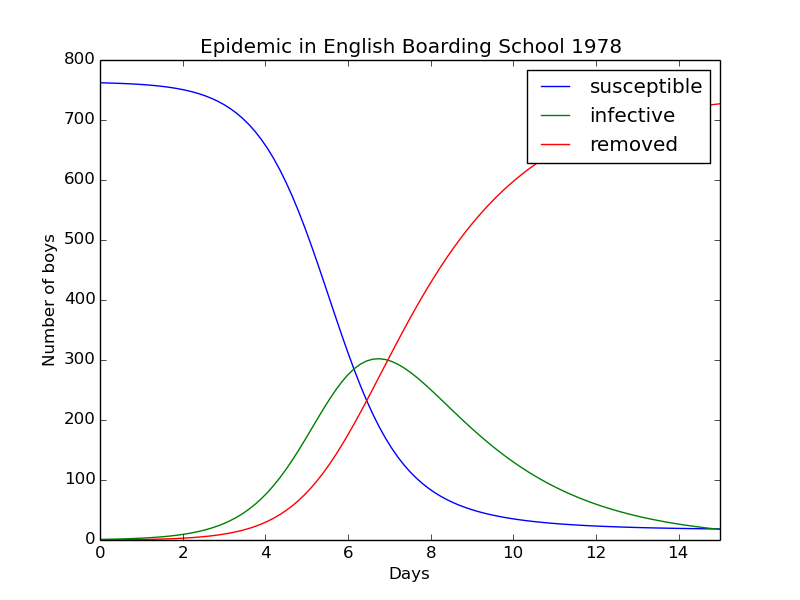
\includegraphics[width=0.9\linewidth]{1_fig/English_boarding_school.png}}
  \caption{
  \label{fig:english_boarding} An English boarding school is modeled for 15 days with the following parameters: $N=763$, $S_0=762$, $I_0=1$, $R_0=0$, $\rho=202$ and $r=2.18 x 10^{-3}$. An increase in the \emph{Infected} group can be seen since $S_0 > \rho$.
  }
\end{figure}
%\clearpage % flush figures fig:english_boarding


\subsection{Maximum concentration of \emph{Infected}}
The maximum concentration of the \emph{Infected} group can be found by usin the threshold value. The result can be compared to the simulation in Fig.(\ref{fig:english_boarding}). Maximum of \emph{Infected} can be found by the following equation from Eq.(\ref{eq:max_I})
\begin{equation} \label{eq:max_I_eng}
\Imax= N - \rho + \rho \ln\frac{\rho}{S_0} 
\end{equation}
By inserting the parameters from the simulation in Fig.(\ref{fig:english_boarding}) in Eq.(\ref{eq:max_I_eng}), the value of $\Imax = 292$. The $\Imax$ of the simulation can be found by checking the maximum number of the infected list. This is similar as the calculated $\Imax$. This maximum value of the \emph{Infeced} group occurs when the $Susceptible$ group is 202, and similar to the value of $\rho$ in the simulation.

\subsection{Variation in parameter value $\rho$}
The parameter value $\rho$ has a major impact on the result. The epidemic disease could turn out quite differently than in the situation in Fig.(\ref{fig:english_boarding}), caused by variations in $a$ and $r$. Fig.(\ref{fig:rho_changes}) consists of some examples where $\rho$ varies from 50 to 400.


\begin{figure}[ht]
  \centerline{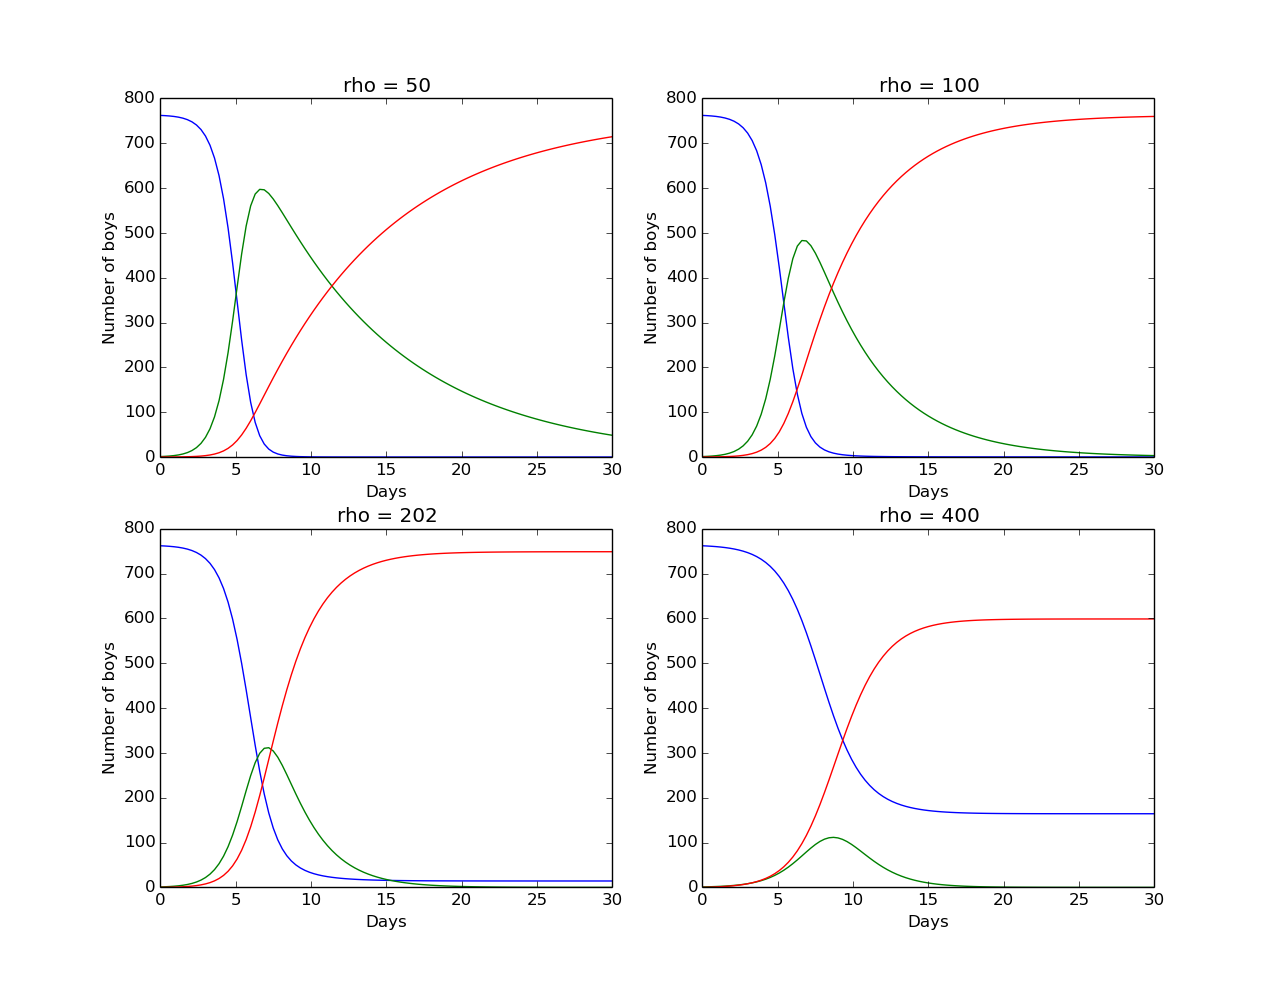
\includegraphics[width=0.9\linewidth]{1_fig/English_boarding_school_changes.png}}
  \caption{
  \label{fig:rho_changes} In the first plot where $\rho=50$, the \emph{Infected} group will increase until the number of \emph{Susceptible} falls down to 50. This will result in a majority of infected students. In the last plot where $\rho=400$, the total number of \emph{Susceptible} stays around 170 students and will go towards a steady number as $I(\infty)=0$.
  }
\end{figure}
%\clearpage % flush figures fig:rho_changes


\section{Zombification}
One of the worst epidemics that can affect the human population is a zombie attack. This will have a huge impact on the way humans live today. Several movies and series has illustrated this type of situation, but it is time that the scientists also take this threat seriously. There have been written a couple of papers about this. Munz et. al\cite{munz2009zombies} used the SEIR model to simulate a possible upcoming zombiefication, where the latent group($E$), is replaced with an \emph{Infected} group($I$) and the \emph{Infected} group($I$) is replaced with a \emph{Zombie} group($Z$). Here it is important to know that the \emph{Infected} group in the $SIZR$ is not the same as in the $SEIR$ model. The following model was used,

\begin{align*}
\frac{dS}{dt} =& \Sigma -\beta SZ - \delta S \\
\frac{dI}{dt} =& \beta SZ - \varrho I - \delta I\\
\frac{dZ}{dt} =& \varrho I + \zeta R - \alpha SZ\\
\frac{dR}{dt} =& \delta S + \delta I + \alpha SZ - \zeta R
\end{align*}

This is a bit more complicated than the standard $SEIR$ model. A presentation of the parameters;
\begin{itemize}
\item $\Sigma$ describes the birthrate for new \emph{Susceptible}. $\frac{dS}{dt}$ is now able to be positive. This is now not a closed system. 

\item $\beta SZ$ describes the numbers of \emph{Susceptible} that become infected , based on interactions between zombies and humans. Similar to the case for $rSI$ in the SIR model. 

\item $\delta$ describes the number of natural deaths in the group. This is used in the \emph{Susceptible} and the \emph{Infected} group

\item $\varrho I$ describes the probability for an infected human to wake up as a zombie.

\item $\zeta R$ controls the number of \emph{Removed} that arises as \emph{Zombie}. 

\item $\alpha SZ$ describes the number of zombies killed by humans in the zombie attacks. 
\end{itemize}

\noindent


\vspace{3mm}




\vspace{3mm}


This model was challenged by Langtangen, Mardal and Røtnes \cite{zombie-math} now referred to as LMR, where they developed another model. They had three objections to the model from Munz et al.~\cite{munz2009zombies}. LMR argue that dead zombies cannot become functioning zombies again. Therefore $\zeta$ will be zero, if magic is not introduced. They let the parameters in the model change with time, according to different phases. LMR argue that the behavior will change with time during a zombie attack. The parameters in the model from LMR was based on the movie \emph{The Night of The Living Dead}. This was done to reproduce its scenarios and then predict how a zombie outbreak would appear. There is also added a function $\omega(t)$, which creates a massive attack from the humans. This is controlled by a time variable and give the \emph{Susceptible} a chance to fight back. The system can be seen in Eq.(\ref{eq:LMR_model}):
\begin{equation} \label{eq:LMR_model}
	\begin{aligned} 
	\frac{dS}{dt} =& \Sigma -\beta SZ - \delta_SS \\
	\frac{dI}{dt} =& \beta SZ - \varrho I - \delta_II\\
	\frac{dZ}{dt} =& \varrho I- (\alpha+\omega(t))SZ + \zeta R\\
	\frac{dR}{dt} =& \delta_SS +\delta_II -\zeta R + (\alpha+\omega(t))SZ 
	\end{aligned}
\end{equation}
The main change is the $\omega(t)$. This is a Gaussian curve and can be seen in eq(\ref{eq:omega}).
\begin{equation} \label{eq:omega}
\omega(t) = a \sum^m_{i=0}\exp\left(\frac{1}{2}\left(\frac{t-T_i}{\sigma}\right)^2\right)
\end{equation}
$\omega(t)$ controls the attacks from the \emph{Susceptible}, which will be fired at predefined time steps. These are controlled by the three parameters. 
\begin{itemize}
\item $a$ here works as a similar parameter as $\alpha$, but will only be activated when the \emph{Susceptible} group is organized and ready to attack. 

\item $T$ contains a list of numbers, which controls the time when the attacks will occur.

\item $\sigma$ controls the length of the attack. 
\end{itemize}

\noindent
This function will be modeled later when it is used in section~\ref{section:counter_attack}


\vspace{3mm}




\vspace{3mm}



\subsection{Parameters used in the model}
The parameter values are essential factors when modelling a zombie attack. Data from the movie \emph{The Night of The Living Dead} was used as basis for the parameters in the ODE system from LMR \cite{zombie-math}. This thesis is based on a thorough study of the TV series \emph{Walking Dead} \cite{walking_dead}. The data will be based on the first five episodes and are constructed after having watched the episodes carefully. The three phases in a zombie attack will be based on the form used in the paper from LMR, but with an extended version in the \emph{Counter attack phase} .

\subsection{The initial phase}
The disease is not yet known in this phase and humans try to save the sick ones by taking them to hospitals or getting some kind of treatment. Because of this ignorance related to the disease, the number in the \emph{Infected} group is high. This phase is often quite short and humans soon start to realise that the risk of getting infected by saving others is really high. \emph{Walking Dead} never shows anything from this phase, but the viewer sees the results when the main character sheriff Rick Grimes wakes up at the local hospital. What he sees is the major damage caused in the initial phase, while the society has moved to the hysterical phase.


\vspace{3mm}




\vspace{3mm}


To determine the values for each group in each phase, the length of Ricks coma is essential. There are several factors that give an indication of the time aspect. When Rick wakes up at the hospital, he has grown a smooth beard of about 1 cm. This would correspond with 1 month in average for a male of European origin. He also has some flowers that have dried out. These also give the impression that some weeks have gone by. The hospital is running on its emergency generator. This would probably not last for many days with a fully operational hospital, but the hospital is as well as shut down when Rick wakes up and can give the emergency generator a longer lifetime. Dr.~Edwin Jenner gives the viewer some information in episode 5 where he tells the videolog that it was 63 days since the epidemic started spreading. By studying the first five episodes in detail, one gets an impression that the time aspect has not been in focus. Therefore the different phases are constructed from the information that has been given. Rick Grimes has probably been in a coma for a month and what he meets the first days will be the basis for the number in each group. The total amount of objects in the model will be based on the number of humans, dead and zombies seen in the first five episodes. 
\begin{itemize}
 \item The number of humans has been estimated to 62. 20 living in the camp with Rick, 40 humans in the old nursing home and the father and son in episode 1. 

 \item The number of dead is estimated to 200. This is based on the amount of dead outside the hospital where Rick woke up. 

 \item The number of zombies are assumed to be 360. These are based on the 30 outside the house of Morgan Jones and his son Duane, 300 zombies in the city Atlanta and 30 zombies attacking the camp. 
\end{itemize}

\noindent
The total number will be 622, and the time aspect aroud a month, which means that these numbers are for the hysterical phase.Over the three first days when Rick is awake, 1 human and 20 zombies are killed in battles. This can be used to find the final number in the initial phase by calculating backwards. By going nine similar periods backwards, the number of killed zombies is 190. The same can be done for humans, which then results in 9 killed humans in this period. The final number for the initial phase can then be set to 71 humans, 540 zombies/infected and 20 dead. This is the same number as for the initial values for the hysterical phase, since the phases are connected.


\vspace{3mm}




\vspace{3mm}


Another issue to discuss is the incubation time. Here there are two examples that can be used. The first transformation from human to zombie happens for the character Amy, who was bit in the arm by a zombie. The transformation happens in about 12 hours. The other example is character Jim who has a slower transformation. This lasts for about two days before the rest of the group leave him alongside the road on their way to CDC(Center for Disease Control). An estimate of the incubation time can be set to 24 hours based on these two transformations.


\vspace{3mm}




\vspace{3mm}


The ODE system in Eq.(\ref{eq:LMR_model})can be used to model the initial phase. The expected results are $S_0 = 621$ and $Z_0 = 1$ while the two other groups are set to zero. The value of $\beta$ can be found with the expression $\beta \Delta t S Z$ from the first ODE equation. After three days about 90 percent of the humans are killed.
\begin{equation}
	\begin{aligned}
	\beta\Delta t S Z &= 0.9 S\\
	3\beta   &= 0.9 \\
	\beta &= 0.3 \\
	\end{aligned}
\end{equation}
The probability of a human being infected will be set to $\beta = 0.3$. The natural death and the birth number is set to 0, since the simulations are performed over short period and for a small group. $\delta_S = \Sigma = 0$. It is quite hard to find similar realistic data for infected humans, so $\delta_I = \delta_S$. Since this is data for the initial phase, zombies are seen as infeteced humans that can be saved. Therefore $\alpha = 0$. And the two last parameters are also zero, $a = \zeta = 0$. The initial phase is modeled in Fig.(\ref{fig:initial_phase_1}):


\begin{figure}[ht]
  \centerline{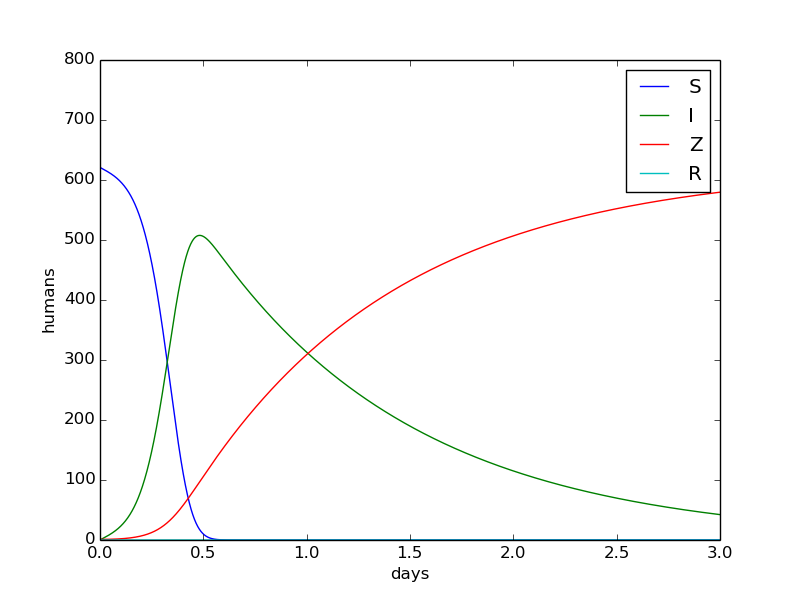
\includegraphics[width=0.9\linewidth]{1_fig/WD_zombie_initial_1.png}}
  \caption{
  \label{fig:initial_phase_1} Initial phase for \emph{Walking Dead}. $\beta=0.3$, $\varrho=1$ and $\alpha=0$ leads to eradication.
  }
\end{figure}
%\clearpage % flush figures fig:initial_phase_1


The result from Fig.(\ref{fig:initial_phase_1}) shows that the human population is eradicated in about a half day. This is not the case, and some adjustments need to be done. There are three parameters that are interesting to study. The first one is $\beta$, which describes how many humans that get infected in a human-zombie collision. The second one is $\varrho$. This parameter controls the incubation time. The last parameter that can affect the number in each group is $\alpha$. This describes the number of zombies killed in a human-zombie collision. These variables are plotted separately and combined in Fig.(\ref{fig:initial_parameters}). The idea here is to produce results that fulfill the final number for the groups \emph{Susceptible} and \emph{Removed} , which is 71 and 20. The blue dot in each plot describes this value. A rough estimate has been done for each parameter before using it. This is why they all lie in different regions than the parameter value in Fig.(\ref{fig:initial_phase_1})



\begin{figure}[ht]
  \centerline{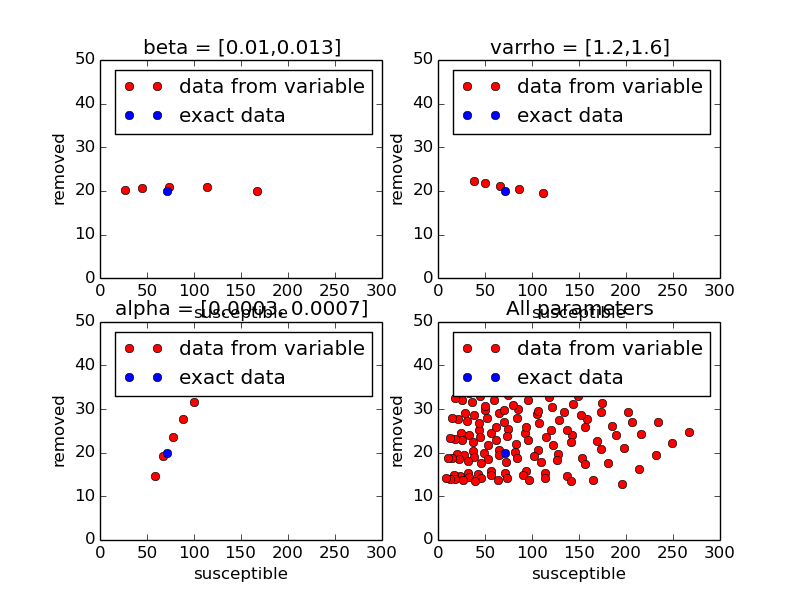
\includegraphics[width=0.9\linewidth]{1_fig/check_parameters.png}}
  \caption{
  \label{fig:initial_parameters} The final result for \emph{Susceptible} and \emph{Removed} group. These plots give a knowledge in the effect of varying the parameters. $\beta$ and $\varrho$ mainly affect the number of \emph{Susceptible} while $\alpha$ affect them both.
  }
\end{figure}
%\clearpage % flush figures fig:initial_parameters


By choosing $\beta = 0.01155$, $\varrho=1.37$ and $\alpha=0.00044$, the following plot can be seen in Fig.(\ref{fig:initial_phase_2}):  


\begin{figure}[ht]
  \centerline{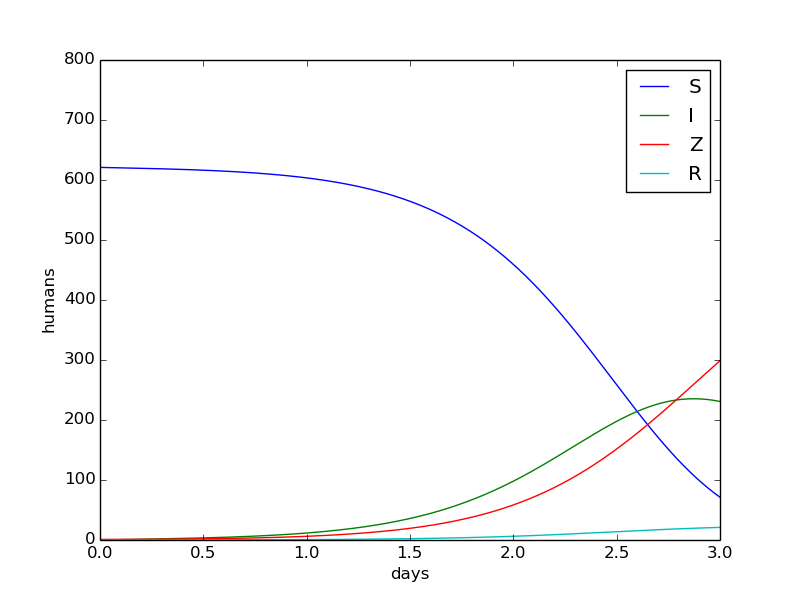
\includegraphics[width=0.9\linewidth]{1_fig/WD_zombie_initial_2.png}}
  \caption{
  \label{fig:initial_phase_2} The final values are $S_n=71.3,I_n=230.8,Z_n=298.9$ and $R_n=21$, which is quite close to the result from the movie.
  }
\end{figure}
%\clearpage % flush figures fig:initial_phase_2


It is possible to argue for the changes done in Fig.(\ref{fig:initial_phase_2}). Increasing $\varrho$ to 1.37 reduces the incubation time. Now the average time will be about 17.5 hours, which is realistic. The probability $\beta$ is sensitive and has a major effect only by small variations. This is due to the term that it is a part of $\Delta t SZ \beta$. A couple of examples demonstrate this. One hour can be estimated by setting $\Delta t = 1/24$. When using the initial values for the groups $S$ and $Z$ and $\beta=0.01155$ from Fig.(\ref{fig:initial_phase_2}). A rough estimate of the \emph{Infected} group in the first hour will be $(1/24)*721*1*0.01155=0.34$. About one-third of a human in the first hour seems as a slow and not very aggressive disease. However when the number of \emph{Zombies} slowly increases, the number of infected will be affected. By looking at the hour when the values are equal between humans and zombies, about 200 in each group, the number of infected will be 19.25 per hour. This result in about 10 percent of the humans. By changing $\beta$ to the value from Fig.(\ref{fig:initial_phase_1}), the number of infected will be 500 per hour and it is quite easy to see that this will lead to eradication in a short amount of time. The last parameter $\alpha$ controls the number of zombies that dies in collisions between zombies and humans. While humans still think that the infected can be saved, it is still a chance that the result from a collision can end with a zombie kill. These results can therefore be seen as realistic values.

\subsection{The hysterical phase}
Now the humans start to avoid the infected and some try to fight them. The humans often gather in groups and try to find safe spots away from the zombies. Important supplies as weapons and food are their main priorities. Barricades are built and the guarding is strict. When Rick Grimes wakes up, the hospital is abandoned and the halls are filled up with dead people. Quite fast he understand that he needs to reach safety. After a couple of days he ends up in a camp outside Atlanta city. A couple of elementary changes has happened with the interaction between humans and infected/zombies. In the initial phase, the humans tried to help the infected humans. This resulted in a high percent of infected. Now they understand this risk and keep distance to those who are infected. This will give $\beta$ a lower value. The morality for a zombie kill has dramatically changed. While this was seen as no option in the initial phase, this is now okay. The humans have started to treat zombies and infected as enemies instead of sick allies. This results in a higher death rate among the zombies, which is described by $\alpha$. 


\vspace{3mm}




\vspace{3mm}


The hysterical model can be constructed based on the data found in the initial phase. 


\begin{quote}
\begin{tabular}{ccc}
\hline
\multicolumn{1}{c}{ hysterical phase } & \multicolumn{1}{c}{ initial values } & \multicolumn{1}{c}{ final values } \\
\hline
S                & 71.3           & 62           \\
I                & 230.8          & -            \\
Z                & 298.9          & 360          \\
R                & 21             & 200          \\
\hline
\end{tabular}
\end{quote}

\noindent
Here, the infected and zombies are counted as one group for the final values, since it is difficult to separate these groups in the series. The time aspect will be modeled for 30 days, which results in a ten times longer simulation. Since the final results are known here, a similar adjustment of the parameters can be done. The range of the parameter values have been found by some test simulations.In Fig.(\ref{fig:hysterical_variations}) the parameters of $\beta$, $\varrho$ and $\alpha$ have been simulated with different values. 


\begin{figure}[ht]
  \centerline{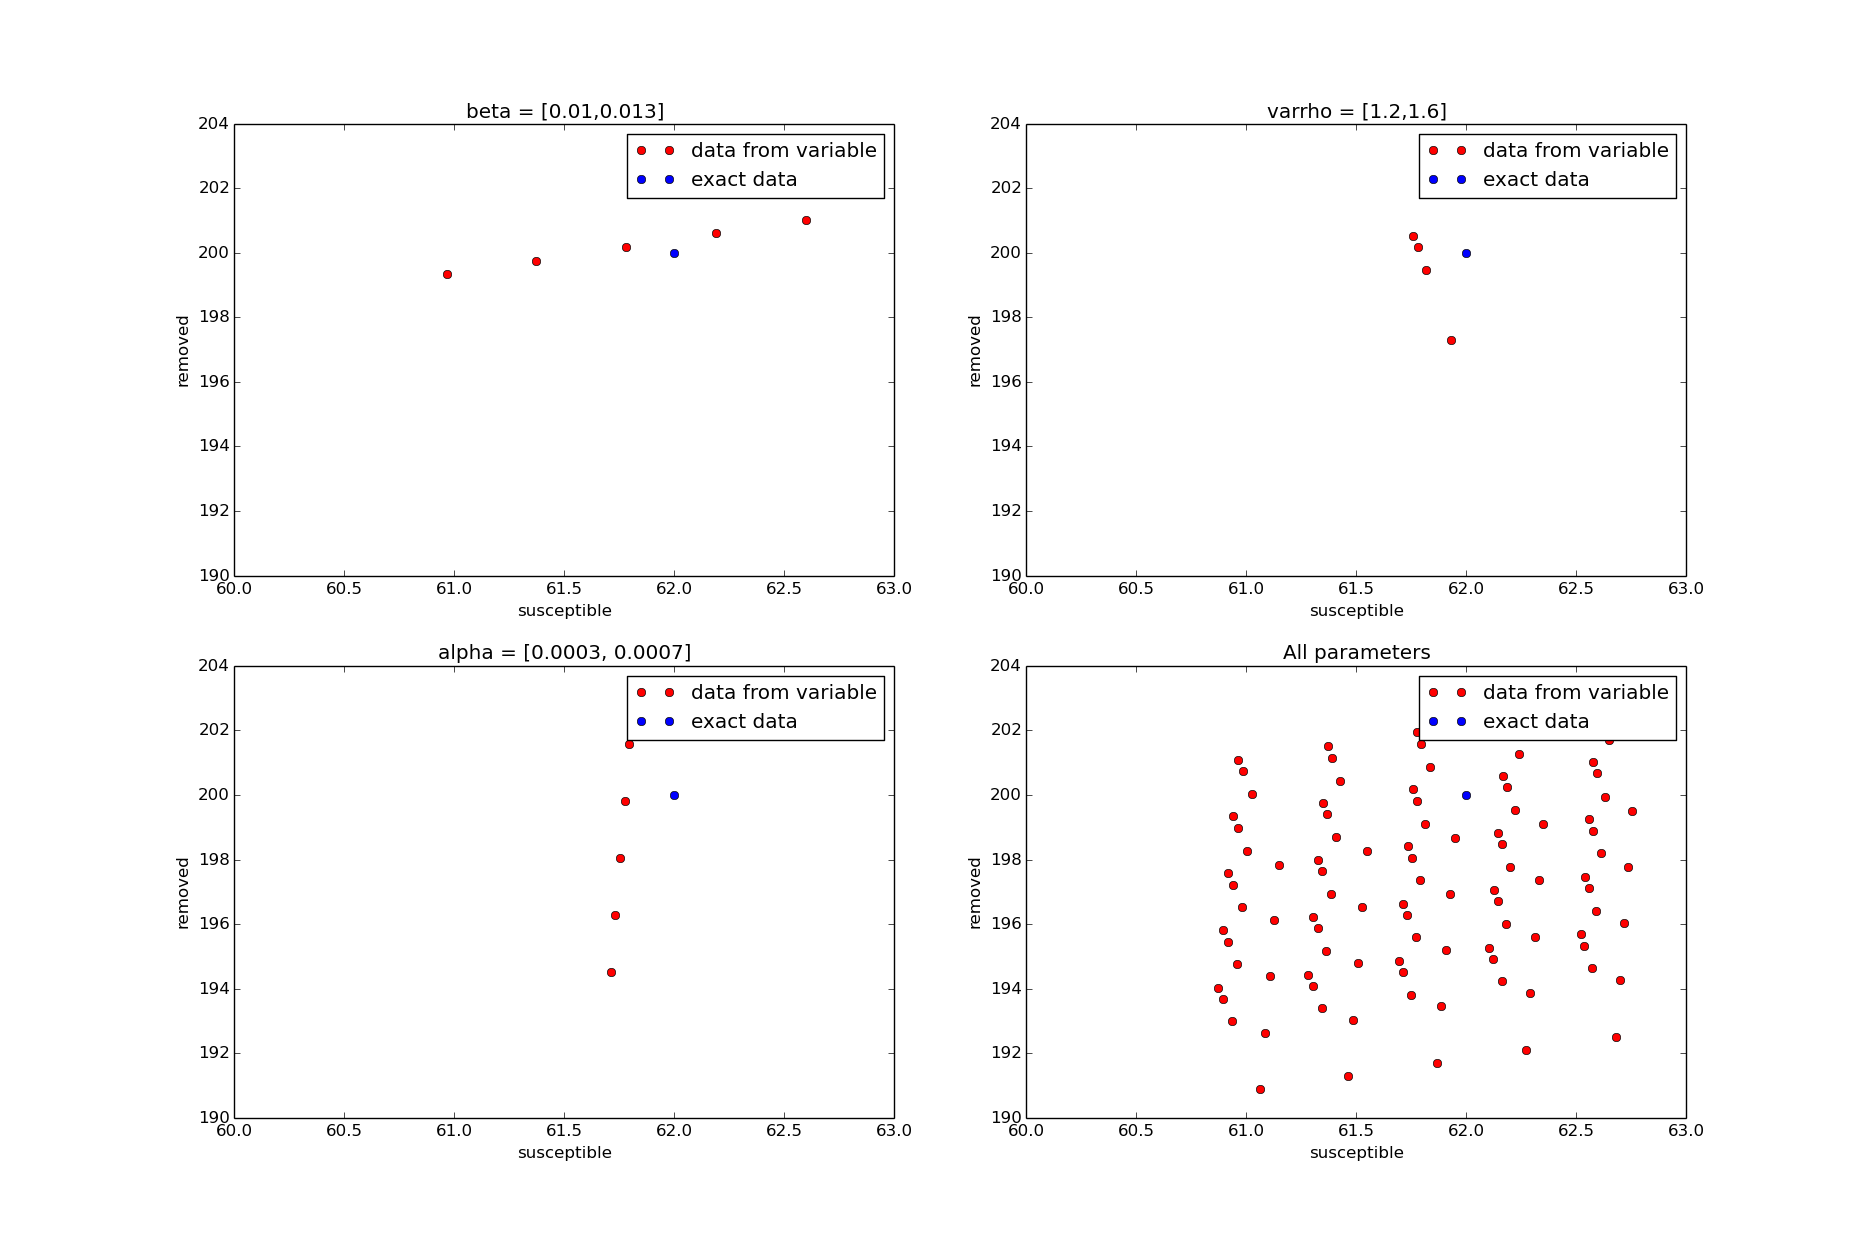
\includegraphics[width=0.9\linewidth]{1_fig/check_parameters_hysterical_2.png}}
  \caption{
  \label{fig:hysterical_variations} Variation in three different parameters in the hysterical phase. The last subplot consist of the combination of all. $\beta=[1\cdot10^{-5},1.2\cdot10^{-5}]$, $\varrho=[1,2]$ and $\alpha=[2\cdot10^{-4},2.2\cdot10^{-4}]$
  }
\end{figure}
%\clearpage % flush figures fig:hysterical_variations


Fig.(\ref{fig:hysterical_variations}) gives insight in how variations in parameters affect the final result. By decreasing $\beta$, it will essentially increase the number of \emph{Susceptible} that will survive, but it will also increase the number of deaths. This may at a first glance seem quite strange. Should not the number of deaths decrease when the number of surviving humans increase? This can be explained with the idea that was shown for $\beta$ in the initial phase. Since $\beta SZ$ gets smaller when $\beta$ gets smaller, the combination of $SZ$ will stay higher for a longer time . This will again affect $\alpha SZ$, which regulates the number of killed zombies. The larger this combination is, the more zombies will die. 


\vspace{3mm}




\vspace{3mm}


By increasing $\alpha$, the number of \emph{Removed} also increase. However similar to the increasing of the \emph{Removed} it also has a slight increase on the number of \emph{Susceptible}. Here the argument for $\beta$ above can be reversed. Since a higher $\alpha$ leads to a higher death rate among the zombies, the combination $SZ$ will be smaller, which makes $\beta SZ$ smaller.


\vspace{3mm}




\vspace{3mm}


The last parameter, $\varrho$, has nearly no effect. The red dots show a small decreasing of \emph{Removed} and increasing of \emph{Susceptible}  when $\varrho$ is increased. This parameter varies most, but has least impact. This can be explained with the long time aspect and the low number of infected compared to the number of zombies. Since the number of zombies is much higher, the transformation length from infected to zombie is almost negligible.  


\begin{figure}[ht]
  \centerline{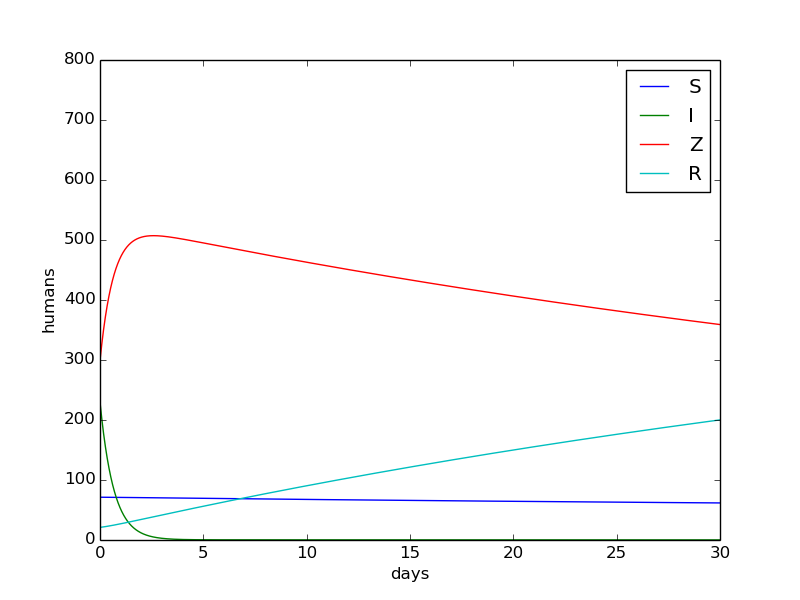
\includegraphics[width=0.9\linewidth]{1_fig/WD_zombie_hysterical_1.png}}
  \caption{
  \label{fig:hysterical_1} Hysterical phase with parameter values $\beta = 0.000011$, $\varrho = 1.5$ and $\alpha = 0.000208$.
  }
\end{figure}
%\clearpage % flush figures fig:hysterical_1


Fig.(\ref{fig:hysterical_1}) fulfills the result that was predicted based on the series. These final numbers correspond with the number in each group when Rick woke up at the hospital. The plot shows that the number of zombies increases quickly and reaches its maximum value after a couple of days in this phase, similar to the number of infected that dramatically decreased. Here the humans have been able to stabilize. Since the clashes between humans and zombies are dramatically decreased, nearly no humans get infected. And in the cases where humans have to face zombies, the killing rate has increased. The increase of \emph{Removed} is close to proportional to the decrease of \emph{Zombies}, which means that it is mostly zombies that die.

\subsection{The counter attack}
\label{section:counter_attack}
This counter attack is more complicated to model, since this phase appears simultaneously as the hysterical phase in \emph{Walking Dead}. The group of humans are trying to avoid the zombies, but when the zombies get too close, the humans need to fight back. These situations are caused by a high density of zombies in some areas, which force the zombies to spread. In \emph{Walking dead} the counter attack appears when a group of 30 zombies reach the camp. This triggers a fight where all the zombies are killed and 4 of the humans get bitten. This shows that a counter attack from the humans causes a lot of damage. The time aspect is set to 6 hours.  


\vspace{3mm}




\vspace{3mm}


Now the function $\omega(t)$ will be used. This can be seen in Fig.(\ref{fig:omega_function}):


\begin{figure}[ht]
  \centerline{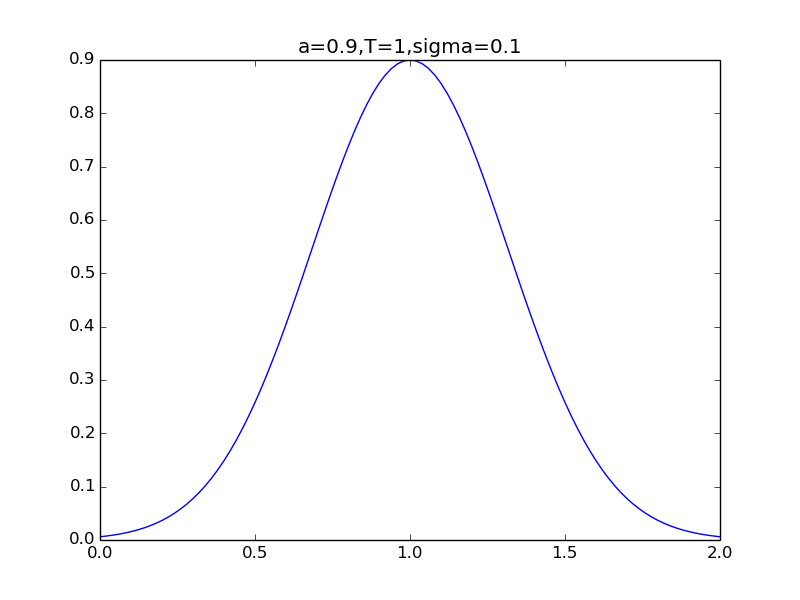
\includegraphics[width=0.9\linewidth]{1_fig/omega_function.png}}
  \caption{
  \label{fig:omega_function} $\omega (t)$ is a Gaussian function where $a$ controls the maximum value, $T$ controls the time for maximum value and $\sigma$ controls the length of the attack.
  }
\end{figure}
%\clearpage % flush figures fig:omega_function


To get some start values, $SZ\omega(t)=30$ can be used. Where $\omega(t)$ is the area under the function. By inserting the final values from hysterical phase for $S$ and $Z$, the area shall be $\omega (t)=1.34\cdot10^{-3}$. This result can be reproduced by using $a= 0.00103$ and $\sigma = 0.005$ in $\omega(t)$. The counter attack is sat to appear during the last part of the day [0.75,1]. The value of T is then set to $T$=[0.875].


\begin{figure}[ht]
  \centerline{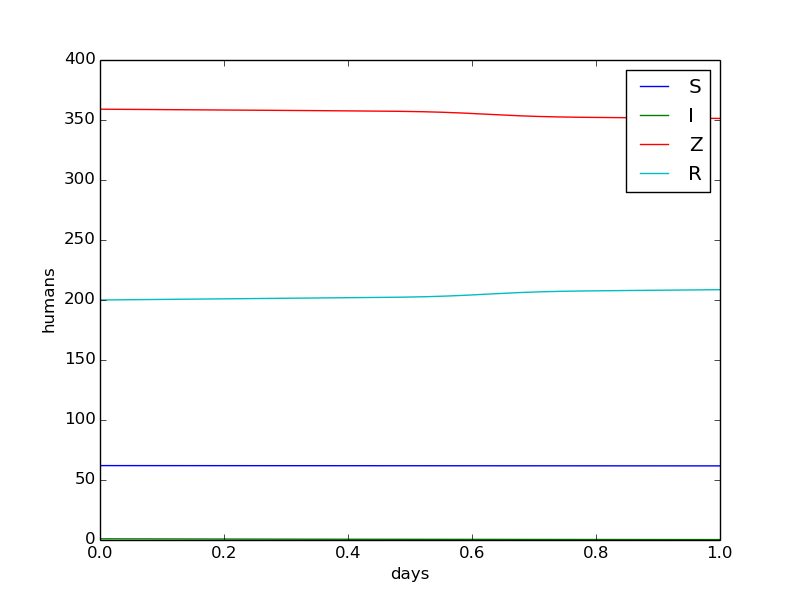
\includegraphics[width=0.9\linewidth]{1_fig/WD_zombie_counter_1.png}}
  \caption{
  \label{fig:zombie_counter_1} The counter attack. 8-9 zombies are killed and all humans survive
  }
\end{figure}
%\clearpage % flush figures fig:zombie_counter_1


This simulation in Fig.(\ref{fig:zombie_counter_1}) results in some deaths. However, the total number should be higher. Another problem is that no humans died during this battle. The ODE model (\ref{eq:LMR_model}) is based on \emph{The Night of the Living Dead}, where the amount of humans who are killed is close to zero. This is not the case in \emph{Walking dead}. Therefore the risk of dying is higher for human during a counter attack. This is solved by adding $\mu \omega (t) SZ$, where $\mu$ is the risk for a human getting infected compared to a zombie kill during this attack. The model (\ref{eq:LMR_model}) can then be expanded to system(\ref{eq:1_seland_model}),

\begin{equation} \label{eq:1_seland_model}
	\begin{aligned} 
	\frac{dS}{dt} &= \Sigma -(\beta+\mu \omega(t))SZ - \delta_SS \\
	\frac{dI}{dt} &= (\beta+\mu \omega(t))SZ - \varrho I - \delta_II\\
	\frac{dZ}{dt} &= \varrho I- (\alpha+\omega(t))SZ + \zeta R\\
	\frac{dR}{dt} &= \delta_SS +\delta_II -\zeta R + (\alpha+\omega(t))SZ 
	\end{aligned}
\end{equation}


\begin{figure}[ht]
  \centerline{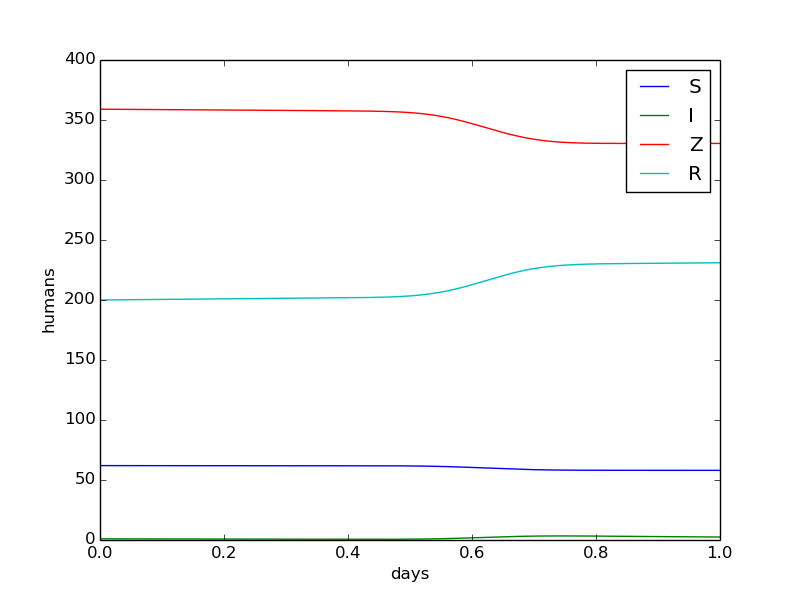
\includegraphics[width=0.9\linewidth]{1_fig/WD_zombie_counter_2.png}}
  \caption{
  \label{fig:zombie_counter_2} Counter attack with the new model. Parameter values are set to $a=0.0073$ and $\mu=0.14$.
  }
\end{figure}
%\clearpage % flush figures fig:zombie_counter_2


Fig.(\ref{fig:zombie_counter_2}) is modeled with the initial values given when Rich woke up, explained in the initial phase. The result after this day is that the humans are reduced to 58 humans. The number in the \emph{Infected} group is increased to 2.47, which can be explained with the two characters in the series, Amy and Jim. The number of \emph{Removed} is increased to 231, and is a combination of killed zombies and humans who are attacked. By modelling this for another day, the \emph{Removed} group will increase with a couple of new deaths. 


\vspace{3mm}




\vspace{3mm}


It would be interesting to check what would happen if this counter attack was repeated over time. Who would survive? An attack every other day will give the following result shown in Fig.(\ref{fig:counter_series})


\begin{figure}[ht]
  \centerline{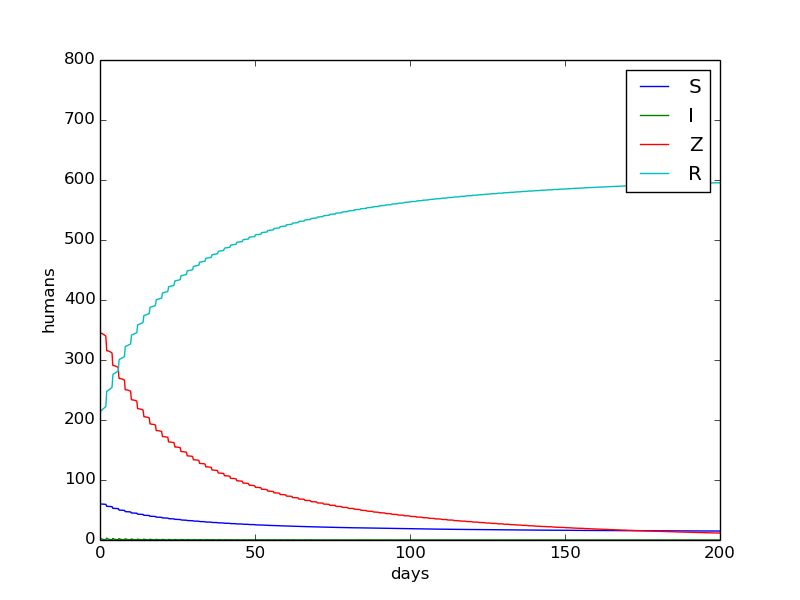
\includegraphics[width=0.9\linewidth]{1_fig/WD_zombie_counter_series.png}}
  \caption{
  \label{fig:counter_series} 100 counter attacks during 200 days will result in a higher population of humans.
  }
\end{figure}
%\clearpage % flush figures fig:counter_series


After 200 days there would be about 15 humans and 12 zombies left. Then the humans would be able to survive since they are more efficient in battles. 

\subsection{The three phases in Walking Dead}
By adding these three phases together, the final result after the attack should be possible to match. The simulation here will be done with the parameters used in the earlier sections. This can lead to a small error since the result of the final number in each phase is given with decimals and the initial values are based on assumptions and round off numbers. The different parameter values are listed in Tab.(\ref{table:param_val}). 

\label{table:param_val}

\begin{quote}
\begin{tabular}{cccc}
\hline
\multicolumn{1}{c}{ parameter } & \multicolumn{1}{c}{ Initial phase } & \multicolumn{1}{c}{ hysterical phase } & \multicolumn{1}{c}{ counter attack } \\
\hline
$\beta$   & 0.01155       & 0.000011         & 0.00011        \\
$\varrho$ & 1.37          & 1.5              & 1.5            \\
$\alpha$  & 0.00044       & 0.000208         & 0.000208       \\
a         & 0             & 0                & 0.0073         \\
$\sigma$  & 0             & 0                & 0.005          \\
$\mu$     & 0             & 0                & 0.14           \\
\hline
\end{tabular}
\end{quote}

\noindent
The simulation is run for 34 days. The three first days are in the initial phase, the resisting days are in the hysterical phase. The counter attack is released on day 33 and lasts for about 6 hours. The plot is shown in Fig.(\ref{fig:all_phases})   


\begin{figure}[ht]
  \centerline{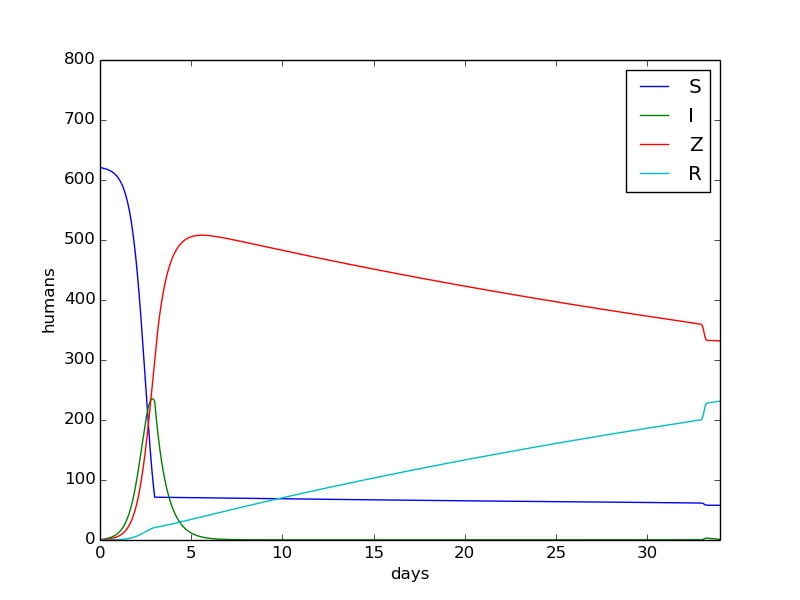
\includegraphics[width=0.9\linewidth]{1_fig/WD_zombie_all_phases_1.png}}
  \caption{
  \label{fig:all_phases} Walking Dead simulated after 5 episodes. Based on the three different phases.
  }
\end{figure}
%\clearpage % flush figures fig:all_phases


Fig.(\ref{fig:all_phases}) clearly shows that the change in parameter values affect the different phases. The different values are shown in the Tab.(\ref{table:group_values}), where the values are given at the initial time. The last column consist of the final values after 34 days.

\label{table:group_values}

\begin{quote}
\begin{tabular}{ccccc}
\hline
\multicolumn{1}{c}{ values } & \multicolumn{1}{c}{ Initial phase } & \multicolumn{1}{c}{ hysterical phase } & \multicolumn{1}{c}{ counter attack } & \multicolumn{1}{c}{ final values } \\
\hline
$S_0$  & 621           & 71               & 62             & 58           \\
$I_0$  & 0             & 231              & 0              & 1            \\
$Z_0$  & 1             & 299              & 359            & 332          \\
$R_0$  & 0             & 21               & 202            & 231          \\
\hline
\end{tabular}
\end{quote}

\noindent
Considering the uncertainty of the parameters, this simulation gives a result close to the expected result. 


\vspace{3mm}




\vspace{3mm}



\section{Discussion}
Two different ODE models are used in this chapter. The first model is a basic SIR model, and the disease in the \emph{English boarding school} is based on this model. The expected result was produced. With variations in the value of $\rho$, it caused large differences in the result for the simulation.


\vspace{3mm}




\vspace{3mm}


The \emph{Zombiefication} part was based on the model and phases from LMR Ref.(\cite{zombie-math}). The parameters and the lenght of the phases were adjusted to simulate \emph{Walking Dead}. Several assumptions were made from the writer to model this series. Since the simulations were based on expected results, the parameters were adjusted to fulfill these demands. The model was able to produce the expected result for the groups, and one can say that the spread can be seen as possible based on these assumptions.    


\vspace{3mm}




\vspace{3mm}


There are several factors that this model don't take into account. How will the number of battles effect the humans and zombies? Will they be tired or more efficient? What about weapons? What would happen if the group of zombies was much larger? Due to different variations in behavior of humans and zombies, one can never predict all situations accurately. This is a weakness with this model, and human behavior is difficult to add to the model.  


\vspace{3mm}




\vspace{3mm}


The parameters found in this model will be used for all three chapters.This model is straight forward to calculate and is easy to use.The model is good if the goal is to find the total amount of each group measured over an area. It demands that the parameters are given. The model gives no information about the spatial spread of the disease. This will therefore be useless in describing how a disease can spread abroad countries and borderlines, or the spatial differences of being infected. The two next chapters will introduce more complicated models which will take the spatial position into account. 


\chapter{PDE models}
This chapter will introduce a spatial model for epidemic diseases. The ODE system from the previously chapter~\ref{section:ODE_models} can be expanded with a term for geographic spread of the disease. The first section \emph{Simple system for spatial spread} will be based on the simple SIR model presented in previously chapter, and the chapter \emph{Geographic spread and Control of epidemics} by Murray \cite{murray2003mathematical}. The parameters from the \emph{English Boarding School} in the previously chapter will be used for the model and the results will be compared. The position of the infected student will be studied to see if it affects the number in the \emph{Infected} group. The last section, \emph{Zombiefication}, will study and expand the system from Langtangen, Mardal and Røtnes \cite{zombie-math}. The results and parameter values used to calculate \emph{Walking Dead} will be compared with the previously ODE system and variations of this PDE. 


\section{Simple system for spatial spread}
A spatial variable, \textbf{x}, will be introduced to the model. This results in both temporal and spatial variations. The difference from a standard ODE system will be the diffusion part added to each equation. The system can be seen in Eq.(\ref{eq:simple_PDE}). 
\begin{equation} \label{eq:simple_PDE}
	\begin{aligned}
	\frac{\partial S}{\partial t} &= -rIS + D\nabla ^2 S\\
	\frac{\partial I}{\partial t} &= rIS- aI + D\nabla ^2 I\\
	\frac{\partial R}{\partial t} &= aI + D\nabla ^2 R
	\end{aligned}
\end{equation}
Here $S$ describes the \emph{Susceptible} group, $I$ describes the \emph{Infected} group and $R$ describes the \emph{Removed} group. The following conditions are set for the boundary and initial values:
\begin{equation} \label{eq:boundary_initial}
	\begin{aligned}
	u_x(0,t) &= u_x(X,t) = 0,\quad u = S,I,R\\
	u(x,0) &= f_u(x),\quad u= S,I,R
	\end{aligned}
\end{equation}
This results in Neumann conditions at the boundary. The following implementation can be used at the boundary
\begin{equation}
	\begin{aligned}
	\frac{u_{-1}^n - u_1^n}{2\Delta x} &= 0 \\
	u_{-1}^n &= u_1^n
	\end{aligned}
\end{equation}
This is solved by adding an extra point on each side, called ghost points. The values in these ghost points are updated every time step with values from $u_1^n$ and $u_{X-1}^n$. All three groups, $S,I,R$ in Eq.(\ref{eq:simple_PDE}) have the same diffusion coefficient, $D$. This gives the three groups the same diffusion speed. This can vary between systems. Later in the chapter, in section \emph{Zombiefication}, different diffusion terms are given to the groups. The two probabilities $rIS$ and $aI$ will work in the same way as in the ODE system. Since this model takes the position into account, a group of \emph{Infected} that move into a uniform population with \emph{Susceptible} can be model. The group of \emph{Susceptible} has the density $S_0$. A simulation can show the geotemporal spread of the disease. The problem can first be considered as one-dimensional. The system can be nondimensionalised by writing 
\begin{equation} \label{eq:constants_nondimensional}
	\begin{aligned}
	I^* =\frac{I}{S_0},&\quad I^* = \frac{I}{S_0},&\quad R^*= \frac{R}{S_0},&\\
	x^* =\left(\frac{rS_0}{D}\right)^{1/2}x,&\quad t^*=rS_0t,&\quad \lambda =\frac{a}{rS_0},&
	\end{aligned}
\end{equation}
$S_0$ is used as a representative population. Now Eq.(\ref{eq:simple_PDE}) can be expressed as in Eq.(\ref{eq:simple_non_PDE}). The asterisks have been dropped to make it easier to read.
\begin{equation} \label{eq:simple_non_PDE}
	\begin{aligned}
	\frac{\partial S}{\partial t} &= -IS + \frac{\partial^2 S}{\partial x^2},\\
	\frac{\partial I}{\partial t} &= IS- \lambda I + \frac{\partial^2 I}{\partial x^2},\\
	\frac{\partial R}{\partial t} &= \lambda I + \frac{\partial^2 R}{\partial x^2},
	\end{aligned}
\end{equation}
The three parameters $r$, $a$ and $D$ have been replaced by $\lambda$. The \emph{reproduction rate} that was presented for the ODE model can be seen as $1/\lambda $.
\begin{equation} \label{eq:reproduction_rate_PDF}
R_0 = \frac{1}{\lambda} = \frac{rS_0}{a}
\end{equation}
The number of secondary infections produced by one primary infected can be seen as $1/\lambda$. It can also be used to measure two different time scales. The first one, $1/(rS_0)$, measures the contagious time of the disease. The second one looks at the life expectancy for an infected. This can be described as $1/a$ \cite{murray2003mathematical}. 
\subsection{Travelling wave 1D}
In this case the travelling wave describes how a group of \emph{Infected} travels through a geographic area of \emph{Susceptible}. This will be shown by sending a pulse from the \emph{Infected} group into a group of \emph{Susceptible}. A travelling wave solution can be described as follows,
\begin{equation} \label{eq:trav_para}
I(x,t)=I(z),\quad S(x,t)=S(z),\quad R(x,t) = R(z),\quad z = x-ct,
\end{equation}
The value $c$ describes the wave speed. This represents a wave of constant shape that travels in the positive x-direction. Eq.(\ref{eq:trav_para}) can be inserted into Eq.(\ref{eq:simple_non_PDE}). This result in the ordinary system Eq.(\ref{eq:ord_diff_sys})
\begin{equation} \label{eq:ord_diff_sys}
	\begin{aligned}
	S'' + cS' - IS &= 0,\\
	I'' + cI' + I(S-\lambda)&=0\\
	R'' + cR  + I\lambda &=0
	\end{aligned}
\end{equation}
This makes an eigenvalue problem. The value of $\lambda$ needs to stay in a range where $c > 0$ is fulfilled. The values $S$, $I$ and $R$ have to stay nonnegative. This leads to
\begin{equation} 
	\begin{aligned}
	0 \leq S(-\infty) < S(\infty)&=1\\
	I(-\infty)=I(\infty)&=0,\\
	1 \geq R(-\infty)\geq R(\infty) &= 0
	\end{aligned}
\end{equation}
An epidemic wave can be seen in Fig.(\ref{fig:1D_sub}). The value of $\lambda$ is set to 0.5. The initial value of \emph{Susceptible} is 1 for the area and the \emph{Removed} is set to 0. The \emph{Infected} group has a Gauss curve around 0 at initial time. In the four subplots in Fig.(\ref{fig:1D_sub}), the epidemic wave travels towards the other side. The value $z$, which is defined in Eq.(\ref{eq:trav_para}), is used to plot the travelling wave measured at a specific point, in this case $x=15$. This travelling wave is shown in figure(\ref{fig:1D_tw}).       


\begin{figure}[ht]
  \centerline{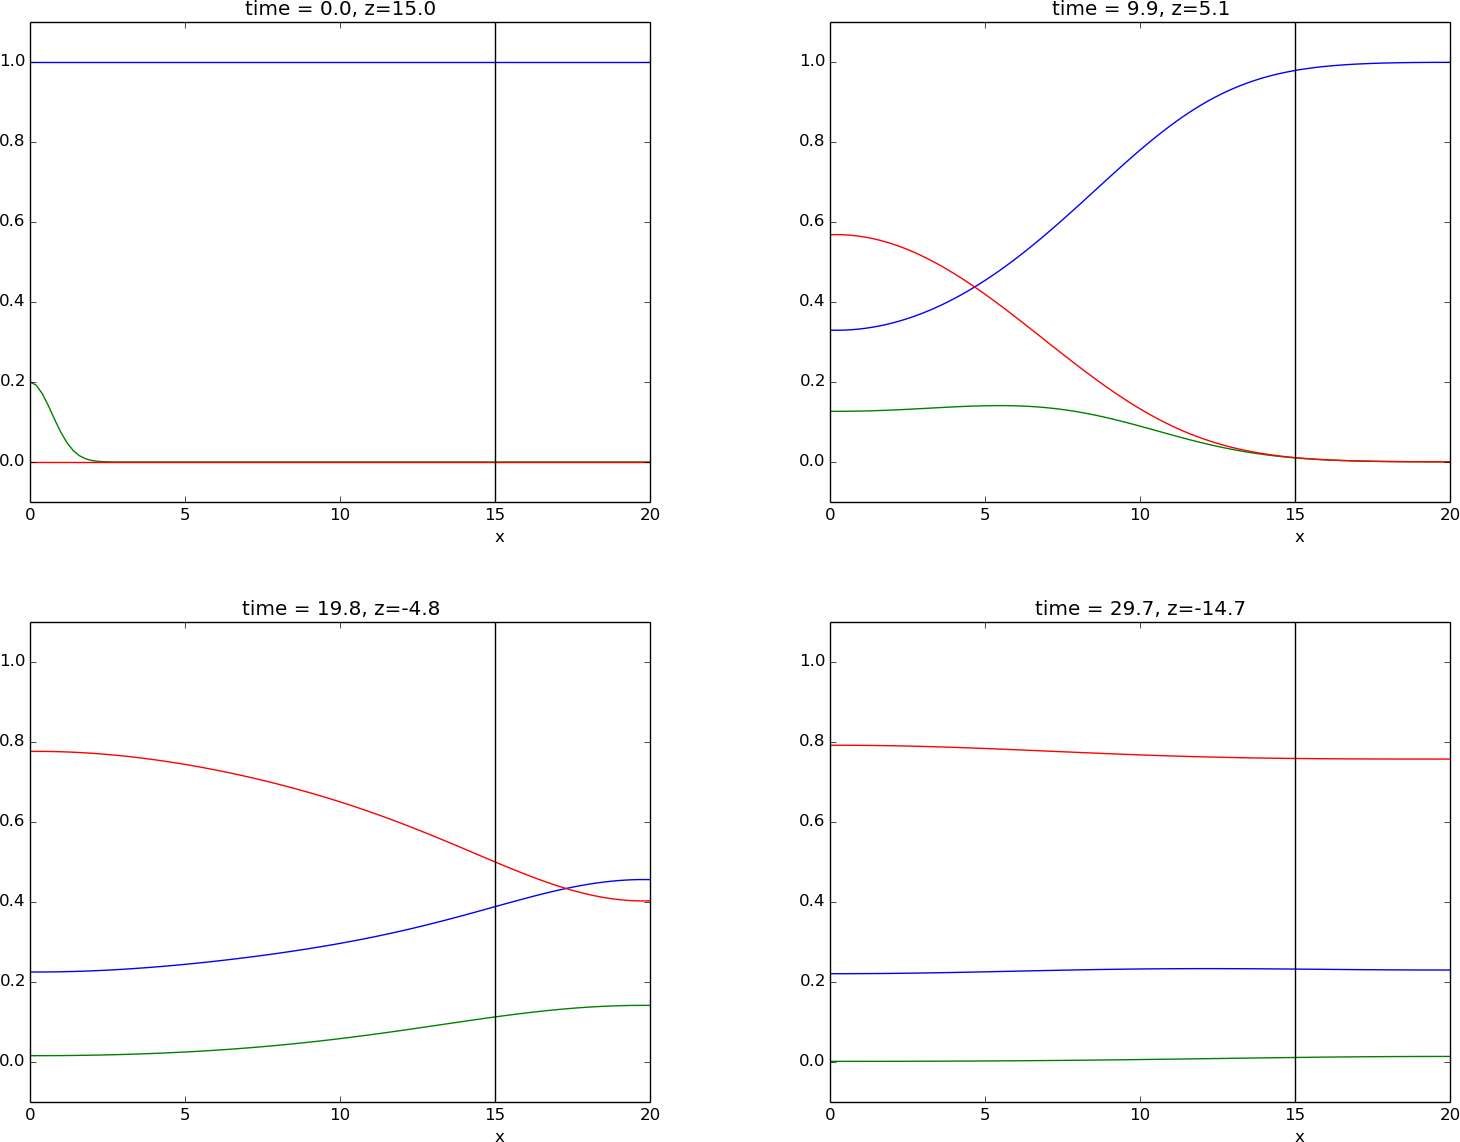
\includegraphics[width=0.8\linewidth]{2_fig/trav_wave_sub.png}}
  \caption{
  \label{fig:1D_sub} The system (\ref{eq:ord_diff_sys}. A gaussian curve with height 0.2 placed on the left side. This causes an epidemic wave controlled by the parameter $\lambda=0.5$. The size is measured at point $x=15$ and can be seen in figure (\ref{fig:1D_tw}).
  }
\end{figure}
%\clearpage % flush figures fig:1D_sub



\begin{figure}[ht]
  \centerline{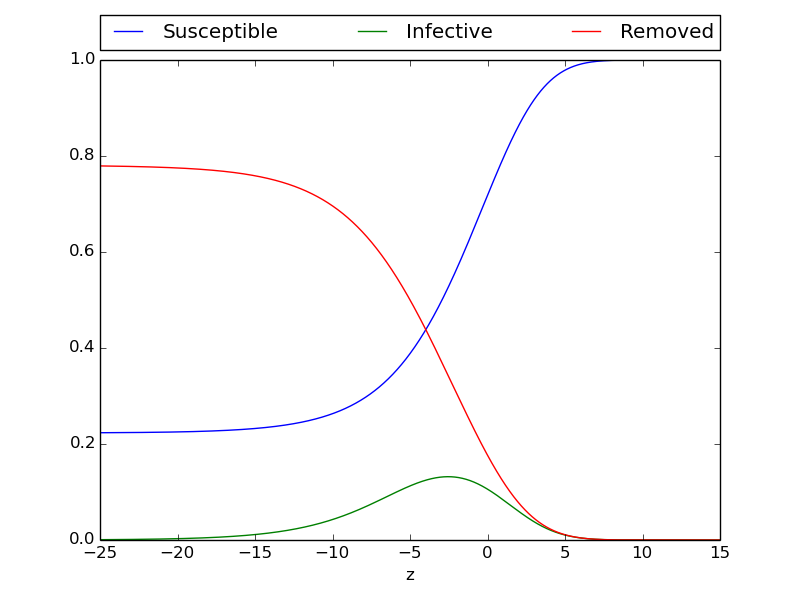
\includegraphics[width=0.9\linewidth]{2_fig/epidemic_wave_z_lambda_0_5.png}}
  \caption{
  \label{fig:1D_tw} This shows the travelling wave measures at at $x=15$ in figure(\ref{fig:1D_sub})
  }
\end{figure}
%\clearpage % flush figures fig:1D_tw




\vspace{3mm}


The \emph{Infective} group in Eq.(\ref{eq:ord_diff_sys}) can be linearised when $z\rightarrow \infty$. This leads to $S\rightarrow 1$ and $I \rightarrow 0$. The result then become 
\begin{equation}
	I'' + cI' + I(S-\lambda) \approx 0 
\end{equation}
This can be found by
\begin{equation}
I(z) \propto \exp\left[(-c \pm {c^2 -4(1-\lambda)}^{1/2})z/2\right]
\end{equation}
Since it is required that $I(z)\rightarrow 0$ and $I(z) > 0$, oscillations around 0 must be prevented. If a travelling wave exist, it has to satisfy
\begin{equation}
	c \geq 2(1-\lambda)^{1/2}, \lambda < 1
\end{equation}
If $\lambda > 1$, no travelling wave will exist. Then the disease will die out. The terms defined in Eq.(\ref{eq:constants_nondimensional}) will give the threshold conditions,
\begin{equation}
	\lambda = \frac{a}{rS_0} < 1
\end{equation}
This is the same value that was given for the ODE model in the previously chapter.
\subsection{Verifying the solution}
To verify the implementation of the solution, a couple of tests can be done one the system in Eq.(\ref{eq:simple_non_PDE}). The system will be tested with a constant solution and a manufactured solution.   

\subsection{Constant solution}
A constant solution uses preproduced constant values for the concentrations $S$, $I$ and $R$. These can be replaced by $S = C_s,I=C_i,R=C_r$. The value of $C_i$ can only be 0 in Eq.(\ref{eq:simple_non_PDE}). This results in a poor test where several bugs can escape. The system can be expanded by adding a term $\beta R$ to the \emph{Susceptible} group and subtracting the same term from the \emph{Removed} group. Then all three values can be tested. The system will then look like this: 
\begin{equation} \label{eq:simple_non_PDE2}
	\begin{aligned}
	\frac{\partial S}{\partial t} &= -IS + \beta R + \frac{\partial^2 S}{\partial x^2},\\
	\frac{\partial I}{\partial t} &= IS- \lambda I + \frac{\partial^2 I}{\partial x^2},\\
	\frac{\partial R}{\partial t} &= \lambda I - \beta R + \frac{\partial^2 R}{\partial x^2},
	\end{aligned}
\end{equation}
By deriving Eq.(\ref{eq:simple_non_PDE2}), the following system Eq.(\ref{eq:constant_PDE}) has to be solved
\begin{equation} \label{eq:constant_PDE}
	\begin{aligned}
	C_iC_s &= \beta C_r \\
	C_iC_s &= \lambda C_i \\
	\lambda C_i &= -\beta C_r 
	\end{aligned}
\end{equation}
The values $\beta$ and $\lambda$ are based on the constants $C_s,C_i,C_r$, which can be chosen freely. Here they are set to $C_s = 1.2,C_i=0.8,C_r=0.6$. This results in $\lambda= C_s = 1.2$ and $\beta= \frac{C_s C_i}{C_r}=1.6$. A test is made in python and can be seen below.

\begin{Verbatim}[numbers=none,fontsize=\fontsize{9pt}{9pt},baselinestretch=0.95]
def test_constant_solution():
    """
    Test problem where u=u_const is the exact solution, to be
    reproduced (to machine precision) by any relevant method.
    """
    def exact_solution(t):
        return C_s,C_i,C_r
    
    def lam(t,x):
        return C_s

    def beta(t,x):
        return (C_s*C_i)/float(C_r)

    #Constant values
    C_s = 1.2
    C_i = 0.8
    C_r = 0.6
    
    #lam = C_s
    #beta = (lam*C_i)/float(C_r)
    
    T = 2; Nt = 200
    X = 20; Nx = 40
    S_1 = np.ones(Nx+3)*C_s
    I_1 = np.ones(Nx+3)*C_i
    R_1 = np.ones(Nx+3)*C_r
    
    t,x,S,I,R = simple_PDE(T,Nx,Nt,X,lam,beta,S_1,I_1,R_1)
    
    S_e,I_e,R_e = exact_solution(t)
    difference = abs(S_e - S).max()  # max deviation
    tol = 1E-14
    assert difference < tol

    difference = abs(I_e - I).max()  # max deviation
    tol = 1E-14
    assert difference < tol

    difference = abs(R_e - R).max()  # max deviation
    tol = 1E-14
    assert difference < tol
\end{Verbatim}

The test was run with no error, and the three constant values were produced correctly. This test is not good enough to qualify the program alone, however an error here would result in a large error in the program. 
\subsection{Manufactured solution}
By constructing a function to each equation in the Eq.(\ref{eq:simple_non_PDE}), a manufactured solution can be created. Here $S$,$I$ and $R$ are pre produced. The system will be
\begin{equation} \label{eq:simple_non_PDE3}
	\begin{aligned}
	\frac{\partial S}{\partial t} &= -IS + \frac{\partial^2 S}{\partial x^2}+f(x,t),\\
	\frac{\partial I}{\partial t} &= IS- \lambda I + \frac{\partial^2 I}{\partial x^2}+g(x,t),\\
	\frac{\partial R}{\partial t} &= \lambda I + \frac{\partial^2 R}{\partial x^2}+h(x,t),
	\end{aligned}
\end{equation}
where $f$, $g$ and $h$ are functions to achieve the expected results for $S$, $I$ and $R$. In this case the functions will be:
\begin{equation}
	\begin{aligned}
	f(x,t) = \frac{\partial S}{\partial t} + IS - \frac{\partial^2 S}{\partial x^2}\\
	g(x,t) = \frac{\partial I}{\partial t} - IS + \lambda I - \frac{\partial^2 I}{\partial x^2}\\
	h(x,t) = \frac{\partial R}{\partial t} -\lambda I - \frac{\partial^2 R}{\partial x^2},
	\end{aligned}
\end{equation}
When choosing the expected function for the groups, it is important that the boundary conditions from Eq.(\ref{eq:boundary_initial}) is fulfilled.
\begin{equation}
    u_x(0,t) = u_x(X,t) = 0
\end{equation}
The quantities have been set to:
\begin{equation}
	\begin{aligned}
    S(x,t) = cos(\frac{\pi}{X}x)t\\
    I(x,t) = cos(\frac{\pi}{X}x)t\\
    R(x,t) = cos(\frac{\pi}{X}x)t
	\end{aligned}
\end{equation}
Now \Verb!sympy! can be used to do the calculations for the three functions $f$, $g$ and $h$. The program can be seen in the Appendix. This results in the following equations seen in Eq.(\ref{eq:manu_func}) 
\begin{equation} \label{eq:manu_func}
	\begin{aligned}
	f(x,t) &= (t^2\cos(\frac{\pi}{X} x) + (\frac{\pi}{X})^2t + 1)\cos(\frac{\pi}{X} x)\\
	g(x,t) &= (\lambda t - t^2\cos(\frac{\pi}{X} x) + (\frac{\pi}{X})^2t + 1)\cos(\frac{\pi}{X} x)\\
	h(x,t) &= (-\lambda t + (\frac{\pi}{X})^2t + 1)\cos(\frac{\pi}{X} x)
	\end{aligned}
\end{equation}
A similar test made for the constant solution can be used here. While the constant test expected a difference on machine precision, this is not the case here. In this test, an expected convergence rate can be measured. The following manufactured test will be

\begin{Verbatim}[numbers=none,fontsize=\fontsize{9pt}{9pt},baselinestretch=0.95]
def test_manufactured_solution(T,Nt,X,Nx):
    
    def exact_solution_S(t,x):
        return np.cos(np.pi*x)*t

    def exact_solution_I(t,x):
        return np.cos(np.pi*x)*t

    def exact_solution_R(t,x):
        return np.cos(np.pi*x)*t


    def beta(t,x):
        return exact_solution_S(t,x)*exact_solution_I(t,x)/exact_solution_R(t,x)
   
    def f(t,x):
        return (t**2*np.cos(np.pi*x) + (np.pi/float(X))**2*t + 1)*np.cos(np.pi*x) 

    def g(t,x):
        return (lam*t - t**2*np.cos(np.pi*x) + (np.pi/float(X))**2*t + 1)*np.cos(np.pi*x)

    def h(t,x):
        return (-lam*t + (np.pi/float(X))**2*t + 1)*np.cos(np.pi*x)
        

    dx = X/float(Nx)
    dt = T/float(Nt)
    S_1 = exact_solution_S(0,np.linspace(0-dx,X+dx,Nx+3))
    I_1 = exact_solution_I(0,np.linspace(0-dx,X+dx,Nx+3))
    R_1 = exact_solution_R(0,np.linspace(0-dx,X+dx,Nx+3))
     
    t,x,S,I,R = simple_PDE(T,Nx,Nt,X,lam,beta,S_1,I_1,R_1,f,g,h)
    S_e = exact_solution_S(t[-1],x)
    I_e = exact_solution_I(t[-1],x)
    R_e = exact_solution_R(t[-1],x)
    
    difference_S = abs(S_e - S).max()  # max deviation
    difference_I = abs(I_e - I).max()  # max deviation
    difference_R = abs(R_e - R).max()  # max deviation

    return difference_S,difference_I,difference_R
\end{Verbatim}

\subsection{Convergence rate}
The program can be controlled by checking the convergence rate. The error term  for this equation can be described as  
\begin{equation} \label{eq:error}
    \epsilon = C_x\Delta x^2 + C_t \Delta t
\end{equation}
With Eq.(\ref{eq:error}), the expected convergence rate can be found for both $\Delta x$ and $\Delta t$. To be able to separate the $\Delta$s, the other value has to be close to eliminated. To study the value $\Delta x$, the following term has to be fullfilled: $\Delta t \ll \Delta x$. This will lead to $C_t\Delta t \approx 0$, and the error term for $\Delta x$ can be found. The opposite thing can  be done for $\Delta t$. A table for the error is produced for different values for $\Delta t = 0.05$ and $\Delta x=0.1$.

\label{table:error_numbers}

\begin{quote}
\begin{tabular}{ccccc}
\hline
\multicolumn{1}{c}{  } & \multicolumn{1}{c}{ $\Delta x$ } & \multicolumn{1}{c}{ $\frac{\Delta x}{2}$ } & \multicolumn{1}{c}{ $\frac{\Delta x}{4}$ } & \multicolumn{1}{c}{ $\frac{\Delta x}{8}$ } \\
\hline
$\Delta t     $       & 9.9E-3     & -                    & -                    & -                    \\
$\frac{\Delta t}{4} $ & 9.9E-3     & 2.5E-3               & -                    & -                    \\
$\frac{\Delta t}{8} $ & 9.9E-3     & 2.5E-3               & 6.1E-4               & -                    \\
$\frac{\Delta t}{16}$ & 9.9E-3     & 2.5E-3               & 6.1E-4               & 1.5E-4               \\
\hline
\end{tabular}
\end{quote}

\noindent
% 0.00988006143376,0.00246039081619,-,-
% 0.00988361769746,0.00246127510994,0.000614719954035
% 0.00988450717896,0.00246149628689,0.000614775174047,0.000153656409034

\subsection{The spatial error}
The Tab.(\ref{table:error_numbers}) gives information about the error when $\Delta t$ and $\Delta x$ are reduced. By studying the row where $\Delta t/16$, the $C_t \Delta t$ can be seen as close to negligible in Eq.(\ref{eq:error}). The error can be expressed 
\begin{equation}
    \epsilon \propto \Delta x^r
\end{equation}
The value is expected to be $r=2$, since centered difference is used in the spatial discretization. By comparing the error for different $\Delta x$, the convergence rate, $r$, can be expressed, 
\begin{equation} \label{eq:conv_rate}
 r_{12} \simeq \frac{\log(\epsilon_1/\epsilon_2)}{\log(\Delta x_1/\Delta x_2)}
\end{equation}
Since the table above has four different error values, these can be used to give three different convergence rates. $\Delta x_1 = \Delta x, \Delta x_2 = \Delta x/2...$. The same notation has been used for the different error values, $\epsilon$.

\begin{quote}
\begin{tabular}{cccc}
\hline
\multicolumn{1}{c}{  } & \multicolumn{1}{c}{ $\epsilon_1/\epsilon_2$ } & \multicolumn{1}{c}{ $\epsilon_2/\epsilon_3$ } & \multicolumn{1}{c}{ $\epsilon_3/\epsilon_4$ } \\
\hline
r & 2.0056                  & 2.0014                  & 2.0004                  \\
\hline
\end{tabular}
\end{quote}

\noindent
Here the rate goes towards 2, and a 2.order convergence rate seems to be fulfilled.
\subsection{The temporal error}
The temporal error is hard to find since the \emph{Stability criteria} expects $\Delta t$ to fulfill the criteria in Eq.(\ref{eq:stability_cr}) to avoid oscillations.
\begin{equation} \label{eq:stability_cr}
 \Delta t \leq \frac{\Delta x^2}{2}
\end{equation}
As a result, $\Delta x \ll \Delta t$ is impossible, because this only leads to an unstable solution. By looking at the column for $\frac{\Delta x}{8}$, the only stable solution is for $\frac{\Delta t}{16}$. Therefore the technique used for the spatial error cannot be used here. 

\subsection{Travelling wave in 2D}
The Eq.(\ref{eq:simple_non_PDE}) can be discretized for a 2D area. This is more realistic when simulating a geographic spread of an epidemic disease. The non dimensional system  can be discretized with Forward Euler in time and centered difference in space
\begin{equation} \label{eq:SIR_disc}
	\begin{aligned}
    \frac{S^{n+1}_{i,j}-S^n_{i,j}}{\Delta t} &= -I^{n}_{i,j}S^{n}_{i,j} + \left(\frac{S^{n}_{i-1,j}-2S^{n}_{i,j}+S^{n}_{i+1,j}}{\Delta x^2}+\frac{S^{n}_{i,j-1}-2S^{n}_{i,j}+S^{n}_{i,j+1}}{\Delta y^2}\right) \\
    \frac{I^{n+1}_{i,j}-I^n_{i,j}}{\Delta t} &= I^{n}_{i,j}S^{n}_{i,j} -\lambda I^{n}_{i,j} + \left(\frac{I^{n}_{i-1,j}-2I^{n}_{i,j}+I^{n}_{i+1,j}}{\Delta x^2}+\frac{I^{n}_{i,j-1}-2I^{n}_{i,j}+I^{n}_{i,j+1}}{\Delta y^2}\right) \\
    \frac{R^{n+1}_{i,j}-R^n_{i,j}}{\Delta t} &= \lambda I^{n}_{i,j}+\left(\frac{R^{n}_{i-1,j}-2R^{n}_{i,j}+R^{n}_{i+1,j}}{\Delta x^2}+\frac{R^{n}_{i,j-1}-2R^{n}_{i,j}+R^{n}_{i,j+1}}{\Delta y^2}\right) 
	\end{aligned}
\end{equation}
The known values can be placed on the right side. The system will then be
\begin{equation}
	\begin{aligned}
    S^{n+1}_{i,j} &= S^{n}_{i,j}+\Delta t\left(-I^{n}_{i,j}S^{n}_{i,j} + \left(\frac{S^{n}_{i-1,j}-2S^{n}_{i,j}+S^{n}_{i+1,j}}{\Delta x^2}+\frac{S^{n}_{i,j-1}-2S^{n}_{i,j}+S^{n}_{i,j+1}}{\Delta y^2}\right)\right) \\
    I^{n+1}_{i,j} &= I^{n}_{i,j}+\Delta t\left(I^{n}_{i,j}S^{n}_{i,j} -\lambda I^{n}_{i,j} + \left(\frac{I^{n}_{i-1,j}-2I^{n}_{i,j}+I^{n}_{i+1,j}}{\Delta x^2}+\frac{I^{n}_{i,j-1}-2I^{n}_{i,j}+I^{n}_{i,j+1}}{\Delta y^2}\right)\right) \\
    R^{n+1}_{i,j} &= R^{n}_{i,j}+\Delta t\left(\lambda I^{n}_{i,j}+\left(\frac{R^{n}_{i-1,j}-2R^{n}_{i,j}+R^{n}_{i+1,j}}{\Delta x^2}+\frac{R^{n}_{i,j-1}-2R^{n}_{i,j}+R^{n}_{i,j+1}}{\Delta y^2}\right)\right) 
	\end{aligned}
\end{equation}
This results in an explicit system, which is easy to code. It consists of known values on the right side and only one unknown value on the left side.
\subsection{A gaussian wave}
In the PDE system for the 1D equation, a Gaussian quantity of infected humans was placed on the left side in the initial value. This resulted in a wave of \emph{Infected} spreading along the x-axis. A similar procedure can be done for the 2D simulation. A couple of simulations have been produced for the 2D system. The first simulation is calculated with a Gaussian function along the points(0,y) for the \emph{Infected} group at initial time. The second simulation has placed the Gaussian function at point(0,0) for the \emph{Infected} group at initial value. Both simulations can be seen in the Appendix.  


\vspace{3mm}




\vspace{3mm}


The size of the epidemic wave can be measured and compared by studying the travelling wave at a certain point. In these two 2D simulations in Fig.(\ref{fig:2D_trav_wave}), the wave are measured in the point (15,15), while the travelling wave in the 1D simulation was measured at point(15). 


\begin{figure}[ht]
  \centerline{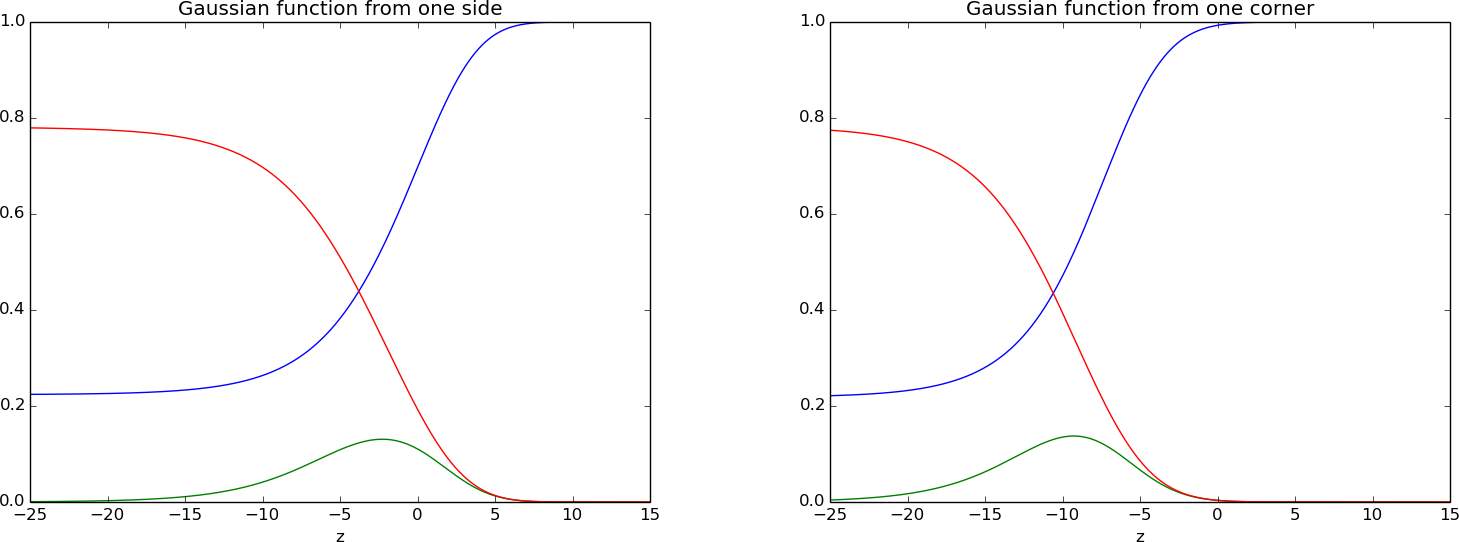
\includegraphics[width=0.8\linewidth]{2_fig/Trav_wave_2D.png}}
  \caption{
  \label{fig:2D_trav_wave} Travelling wave measured at point (15,15) with two different initial values for the \emph{Infected} group. I:The initial value is set as a Gaussian line along (0,y).II:The initial value is set as a Gaussian point (0,0).
  }
\end{figure}
%\clearpage % flush figures fig:2D_trav_wave




\vspace{3mm}




\vspace{3mm}


The shapes of the two travelling waves in Fig.(\ref{fig:2D_trav_wave}) are similar. The only difference is the time when the wave occurs. The plot for 1D wave in Fig.(\ref{fig:1D_tw}) has the same shape. With a closer study, the area under the function can be measured in all three cases. The result can be seen in Tab.(\ref{table:wave_values})   

% 1D
% 1.4340793845
% 1.43143259034 dt = $1\cdot10^{-3}$, dx = 0.05
% 1.43195870243 dt = 0.0002, dx^2 = 0.000625
% 2D wave line:
% 1.43345609926 dt =0.0004, dx^2 =  0.0016
% 2D wave point:
% 1.43352971688

\label{table:wave_values}

\begin{quote}
\begin{tabular}{ccc}
\hline
\multicolumn{1}{c}{ 1D wave } & \multicolumn{1}{c}{ 2D wave line } & \multicolumn{1}{c}{ 2D wave point } \\
\hline
1.43    & 1.43         & 1.43          \\
\hline
\end{tabular}
\end{quote}

\noindent
The area in all three simulations approach the same area when $\Delta t$ and $\Delta x$ are reduced. The size and shape will not change by  expanding the system from 1D to 2D. However, by studying Fig.(\ref{fig:2D_trav_wave}), one can see that the wave occurs at different times. This is caused by the distance from the start position for the Gaussian wave. The first subplot that starts with a Gaussian function along the $x=0$ axis gets a wave from the \emph{Infected} group that flows along the x axis. This can be seen as a wave on the beach. Everyone that have the same distance from the ocean will be hit simultaneously. The travelling wave for the 1D simulation and the first subplot occurs at the same time, because they are measured at the same distance from the starting point. The last plot is also measured at (15,15), but occurs later. Since the wave starts at point (0,0), the distance to (15,15) is 21.21. This means that the wave will reach the point 6.21 time steps later. This is a reasonable conclusion based on the plot.    

\paragraph{Change in initial flow.}
By increasing the initial wave of the \emph{Infected} group, the initial value of \emph{Infected} can be studied. The simulation is run with the same parameters as for the three simulations above and the only difference is the initial value for the \emph{Infected} group. The Gaussian wave of \emph{Infected} is placed at point(0,0) as for subplot II in Fig.(\ref{fig:2D_trav_wave}). The simulation can be seen in Fig.(\ref{fig:initial_value}).  
% Volume ordinary = 0.3141592653589793
% Volume extreme = 157.07963267948966
% Volume under graph 1.43345609926


\begin{figure}[ht]
  \centerline{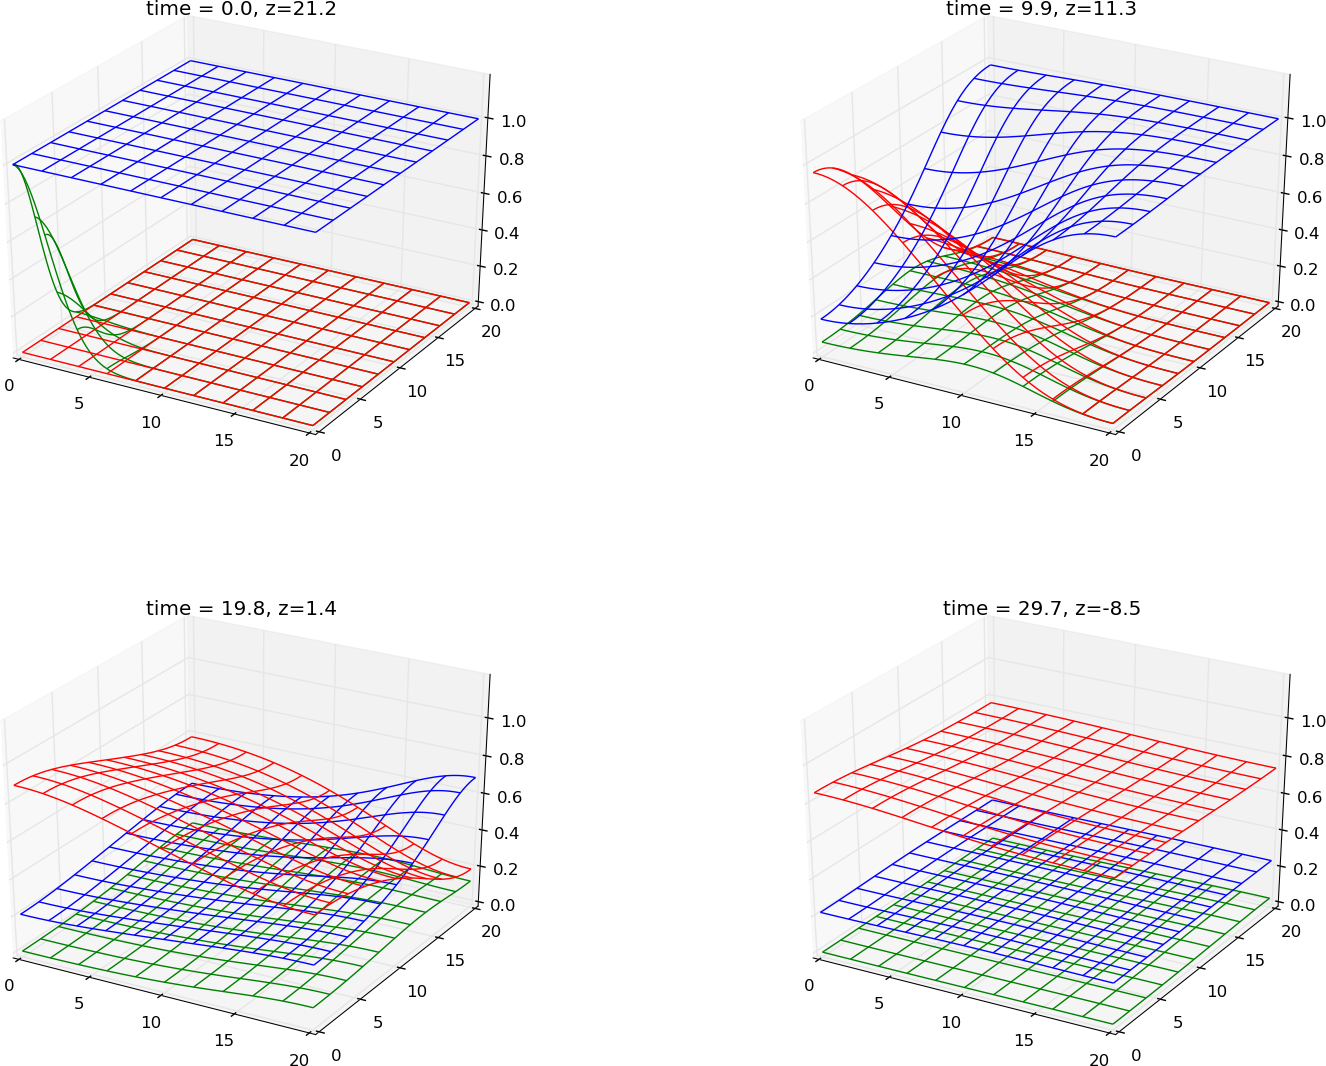
\includegraphics[width=0.8\linewidth]{2_fig/2D_initial_variable_sub.png}}
  \caption{
  \label{fig:initial_value} A major flow of \emph{Infected} spread outwards in the field. After a certain time, the wave has passed the area and the number in each group stabilized.
  }
\end{figure}
%\clearpage % flush figures fig:initial_value




\vspace{3mm}




\vspace{3mm}


The size and shape can be compared by measuring the travelling wave at point(15,15). The travelling wave for this simulation can be seen in Fig.(\ref{fig:initial_trav_wave}) and the area for the travelling wave is measured to 1.43, which is similar to the three other simulations.


\begin{figure}[ht]
  \centerline{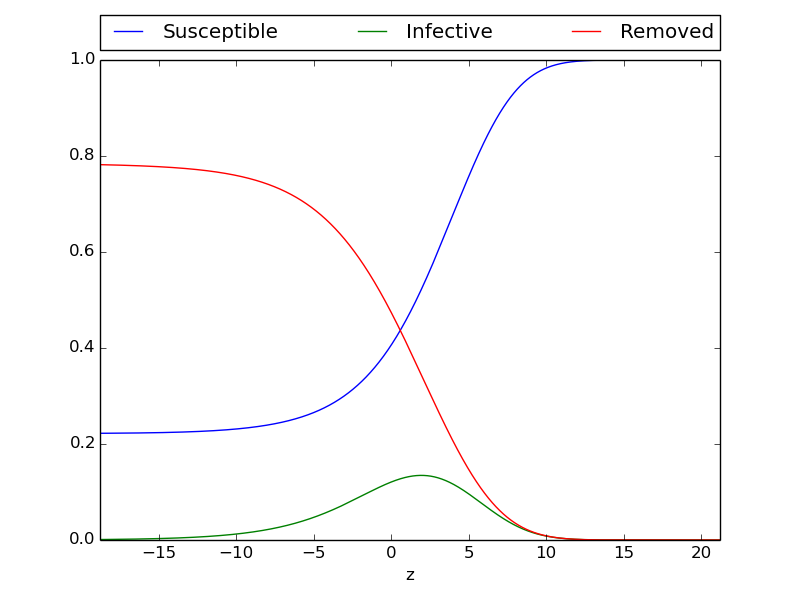
\includegraphics[width=0.8\linewidth]{2_fig/TW_2D_initial_z_lambda_0_5.png}}
  \caption{
  \label{fig:initial_trav_wave} The travelling wave with a major increase of \emph{Infected} at the initial time.
  }
\end{figure}
%\clearpage % flush figures fig:initial_trav_wave




\vspace{3mm}




\vspace{3mm}


The size of the travelling  wave will not be affected by changing the value of the \emph{Infected} group. However there is a difference in the time when the wave occurs. In the simulation where the initial value is higher, the travelling wave reaches the measuring point (15,15) earlier. This can be explained by the idea of a ball dropped from a large height. If the ball is released or thrown to the ground, it will only affect the acceleration of the ball, not the terminal velocity. After a certain time the released ball and the thrown ball will reach the same maximum speed. This is the case for the speed of the travelling wave. 
\paragraph{Change in lambda.}
The one thing that affects the speed and size, is the $\lambda$ variable in the PDE system(\ref{eq:simple_non_PDE}). This $\lambda$ is a combination of $a$, which controls deaths among the \emph{Infected} group, $r$, which controls the number from the \emph{Susceptible} group that gets infected in meetings between the \emph{Infected} and \emph{Susceptible} groups. The last parameter in $\lambda$ is the concentration of Susceptible, $S_0$. By changing this parameter, the travelling wave will change in both size and shape. In Fig.(\ref{fig:change_lambda}), the simulation is run with four different values of $\lambda$.


\begin{figure}[ht]
  \centerline{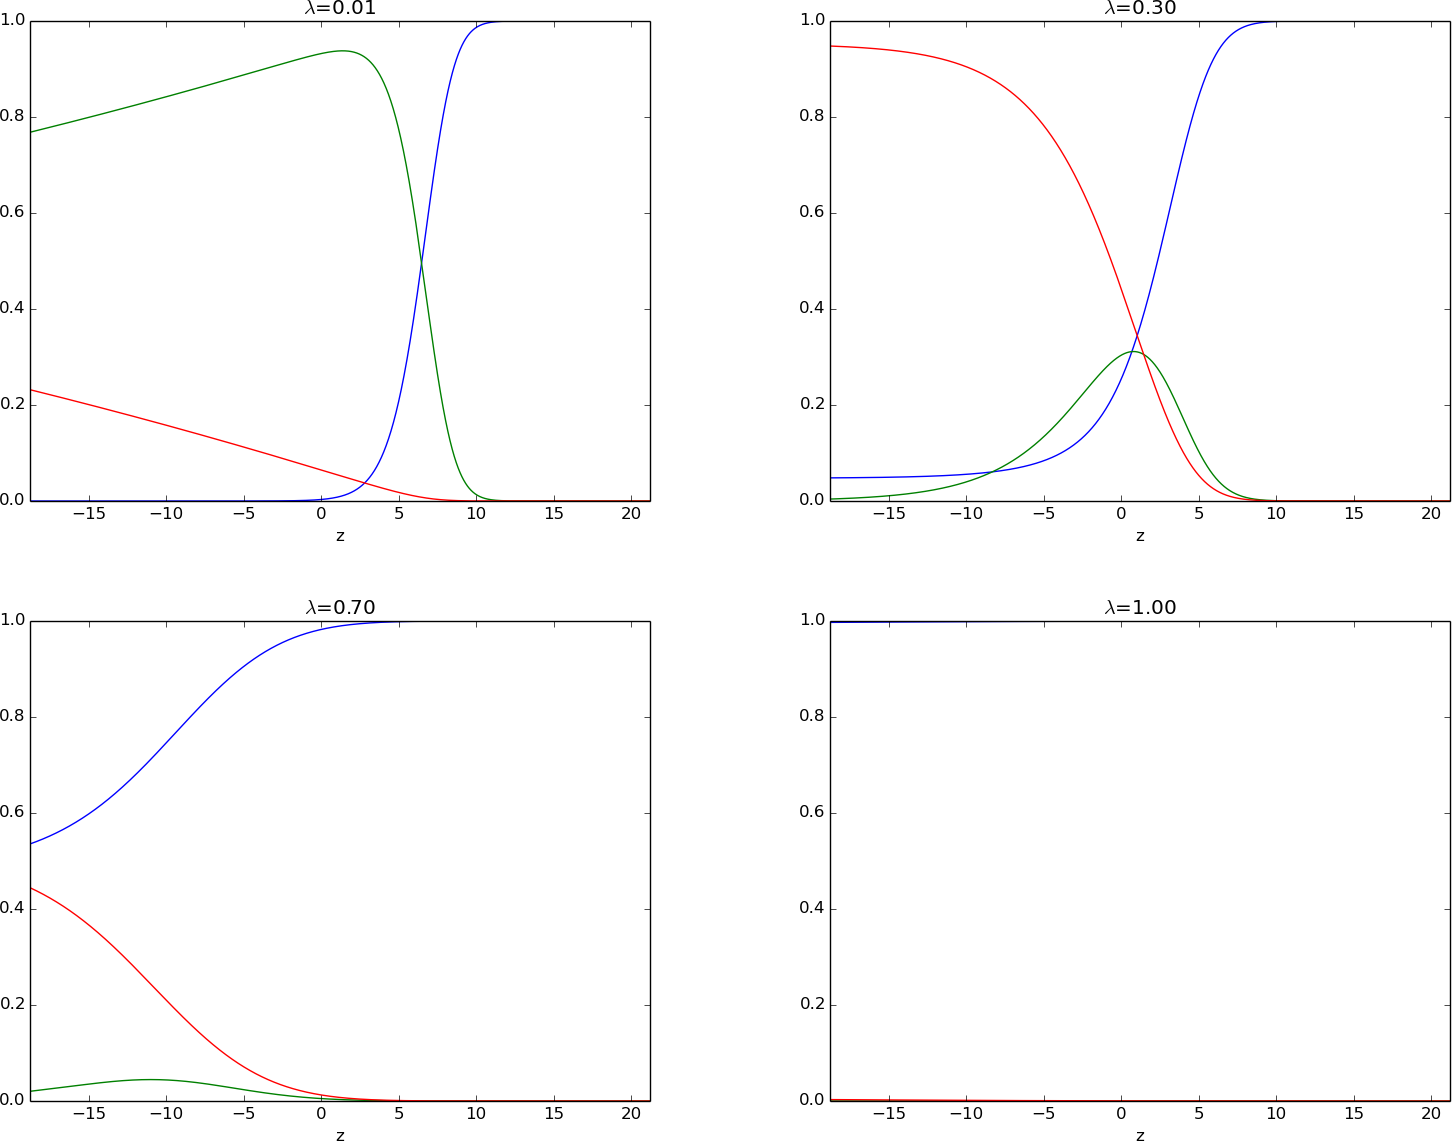
\includegraphics[width=0.9\linewidth]{2_fig/2D_lambda_variable.png}}
  \caption{
  \label{fig:change_lambda} The travelling wave simulated with $\lambda$ values in the range of 0.01 to 1.
  }
\end{figure}
%\clearpage % flush figures fig:change_lambda




\vspace{3mm}




\vspace{3mm}


To understand the results in Fig.(\ref{fig:change_lambda}), the $\lambda $ function can be studied,
\begin{equation} \label{eq:lambda}
 \lambda =\frac{a}{rS_0},
\end{equation}
A major and aggressive travelling wave is caused when $\lambda \rightarrow 0$. In Fig.(\ref{fig:change_lambda}), $\lambda$ is run with value 0.01 in the first subplot. This results in a travelling wave of \emph{Infected} that eradicates the \emph{Susceptible} group in a short time. The wave starts decreasing when all \emph{Susceptible} are infected. By looking at Eq.(\ref{eq:lambda}),one can see that a small value is caused by a small $a$ compared to $r$ and $S_0$. If $a$ is low, this results in few deaths/immune in the \emph{Infected} group. This means that the \emph{Infected} group will grow and be able to infect even more humans from the \emph{Susceptible} group. The same thing will happen if $r$ is large. A result of a large $r$ will be an aggressive disease that infects  a major part of the population. The same result will happen if $S_0$ is large. Then there are several possible humans to infect. Therefore an outburst of a disease is more critical in a crowded city than in the wilderness, far from other humans.


\vspace{3mm}




\vspace{3mm}


If $\lambda$ increases above 1, the disease will not be able to spread. The number of \emph{Infected} will decrease, since the number in the \emph{Removed} group caused by the \emph{Infected} group is higher than the amount of \emph{Infected} humans from the \emph{Susceptible} group. After a certain time, the number of \emph{Infected} will die out. If $\lambda$ stays at 1, the number of \emph{Infected} will be equal the whole time. 

\section{English Boarding School}
An example from an English boarding school was presented in the previously chapter \emph{Epidemic models} . This example was based on the book from J.D Murray \cite{murray2002mathematical}, and was modeled for an ODE system. A similar result should appear for the PDE system with the same parameter values and a uniform distribution of the groups. The school had 763 students, and one of the students brought a disease back to the school. The following numbers were used for the ODE system in chapter one. $N=763, S_0=762,I_0=1,R_0=0,\rho=202$ and $r = 2.18\cdot 10^{-3}$. 


\vspace{3mm}




\vspace{3mm}


The first simulation is produced with uniform distributed concentration, This is done to verify the implementation. A person is defined as one cubic. The total volume of the whole group is spread over the area. The area is set to be 100 m x 100 m, which results in an average height of $1/10000$ m per person. This is done to get a uniformed distribution. This would of course be more difficult in real life, particularly if the person would be alive. Since the \emph{Infected} group only consists of one person, the total height will be 0.0001 for the whole area. The \emph{Susceptible} group consists of 762 students and the total height at each point will be 0.0762 The simulation can be seen in the Appendix. 


\vspace{3mm}




\vspace{3mm}


The results from subplot I in Fig.(\ref{fig:british_number}) are equal to the results from the ODE system modeled in the previously chapter.This can be seen in Tab.(\ref{table:british_number_table}). This is as expected, since the diffusion term is negligible in this system. The simulation results in a group of separate ODE systems modeled over an area.


\begin{figure}[ht]
  \centerline{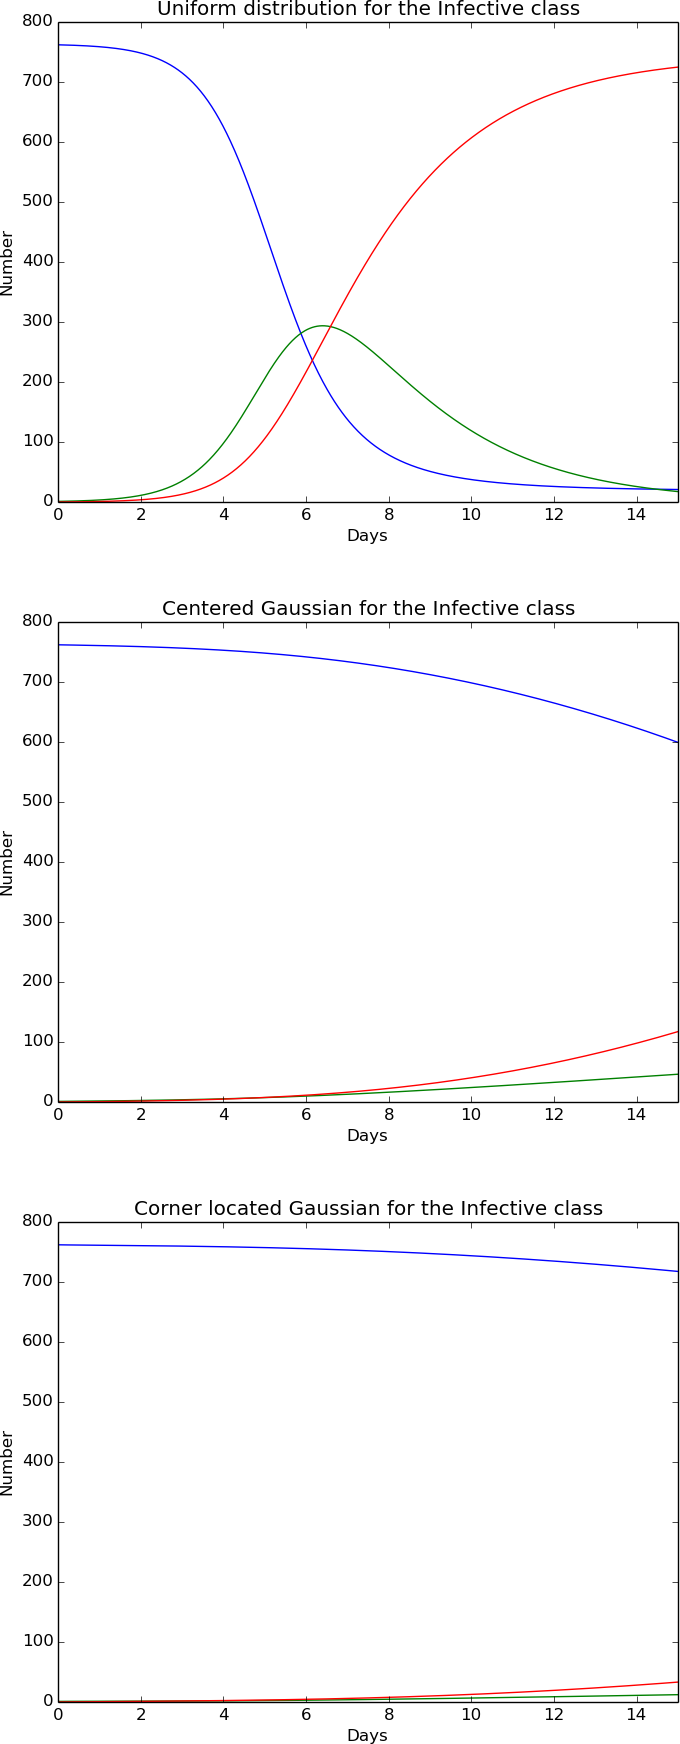
\includegraphics[width=0.6\linewidth]{2_fig/british_number.png}}
  \caption{
  \label{fig:british_number} English Boarding School modeled with three different initial values for the infected student. The amount of students in each group modeled over 15 days. Subplot 1: uniform distribution. Subplot 2: The student is placed as a Gaussian function in center. Subplot 3: The student is placed as a Gaussian function in the corner (0,0).
  }
\end{figure}
%\clearpage % flush figures fig:british_number


\subsection{Maximum concentration of \emph{Infected}}
The maximum concentration of the \emph{Infected} group was found for the ODE system in the previous chapter. The expected value of $\Imax$ was first calculated, and later verified with the numberical solution of the ODE system. The reproduction rate found for the PDE system in Eq.(\ref{eq:reproduction_rate_PDF}) was given by the same parameters as for the ODE system. A similar maximum value is expected from the PDE solution. The maximum value for the \emph{Infected} array is $\Imax=292$ and is similar to the $\Imax$ for the ODE solution. 

A table with the values from the three simulations performed for this English boarding school are compared to ODE system from chapter~\ref{section:ODE_models}.

\label{table:british_number_table}

\begin{quote}
\begin{tabular}{ccccc}
\hline
\multicolumn{1}{c}{  } & \multicolumn{1}{c}{ ODE system } & \multicolumn{1}{c}{ PDE uniform dist } & \multicolumn{1}{c}{ PDE center } & \multicolumn{1}{c}{ PDE corner } \\
\hline
5 Days      & ----------- & ------------------- & ----------- & ----------- \\
\hline
Susceptible & 444.62      & 444.62              & 748.03      & 757.33      \\
Infective   & 209.56      & 209.56              & 7.36        & 2.35        \\
Removed     & 108.82      & 108.82              & 7.60        & 3.32        \\
\hline
10 Days     & ----------- & ------------------- & ----------- & ----------- \\
\hline
Susceptible & 37.59       & 37.59               & 697.71      & 743.58      \\
Infective   & 117.59      & 117.59              & 24.43       & 6.66        \\
Removed     & 607.82      & 607.82              & 40.86       & 12.76       \\
\hline
15 Days     & ----------- & ------------------- & ----------- & ----------- \\
\hline
Susceptible & 21.09       & 21.09               & 597.01      & 717.02      \\
Infective   & 17.30       & 17.30               & 46.96       & 12.37       \\
Removed     & 724.62      & 724.62              & 119.03      & 33.61       \\
\hline
\end{tabular}
\end{quote}

\noindent
% dx = 0.04
% dx^2 = 1.6E-3
% ODE = 1.5E-4

\subsection{Introducing a Gaussian distribution of infected}
An assumption one can make is that a person is not able to be evenly distributed over an area. In this example, with only one infected student at initial time, the chance of being infected increases the closer the \emph{Susceptible} group gets the infected student. The student is represented by a Gaussian function in the middle of the school yard, to see if the position affects the result. The height is set to 1 and the volume of the Gauss function is set to 1 cubic. The simulation can be seen in Fig.(\ref{fig:gauss_sub}) and the total amount of students in each group can be be seen in Fig.(\ref{fig:british_number}).


\begin{figure}[ht]
  \centerline{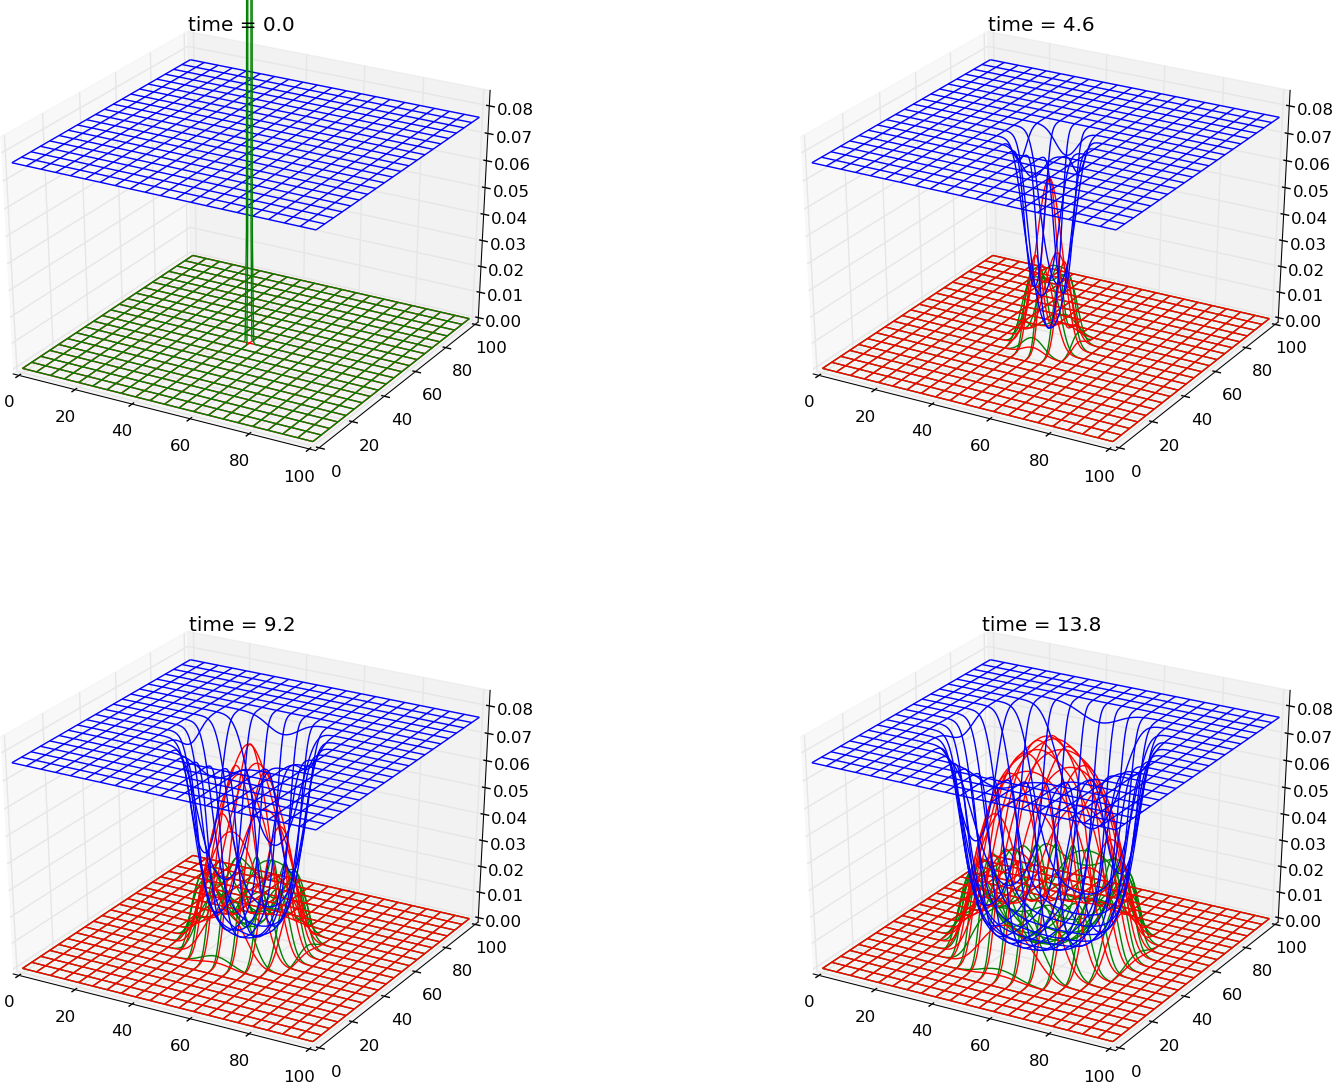
\includegraphics[width=0.8\linewidth]{2_fig/2D_british_school_gauss_sub.png}}
  \caption{
  \label{fig:gauss_sub} The infected student is placed in the center as a Gaussian function at initial time. The height of the Gaussian function is set to 1 m and volume is set to 1 cubic.
  }
\end{figure}
%\clearpage % flush figures fig:gauss_sub




\vspace{3mm}




\vspace{3mm}


The results from the uniform distributed and Gaussian distributed simulations show various results. The initial position of the \emph{Infected} group is the difference between the simulations. This has a major impact. Since the only ones that can be infected by the Gaussian distribution are the students close to the infected student, this restricts the spread of the epidemic. The chance of getting infected in this area is higher. The Fig.(\ref{fig:gauss_sub}) shows that the amount of \emph{Infective} quickly grows in the center, where the infected was placed. Subplot IV in Fig.(\ref{fig:gauss_sub}) shows that the amount from the \emph{Removed} group in the center is close to the maximum of the initial value of \emph{Susceptible}, while the students along the boundary of the schoolyard seem to be unaffected after 15 days. This simulation shows that the position of the \emph{Infected} group has a major role in the simulation.


\vspace{3mm}




\vspace{3mm}


The position of the \emph{Infected} group, here as a Gaussian function, also affects the outcome. Subplot III in Fig.(\ref{fig:british_number}) describes a simulation where the Gaussian function is placed in the corner with position(0,0). The total volume of the function is increased to 4 since only a quarter of the function is placed in the area. Tab.(\ref{table:british_number_table}) shows that the total number of \emph{Infected} is lower than for the centered placed Gaussian function. The infected student is only able to spread the disease to a quarter of the population compared to the infected student in the center. The simulation can be seen in the Appendix.


\vspace{3mm}




\vspace{3mm}


If the simulations are run for a long time, the difference between each group will decrease. After 100 days there will be about 18 students in the \emph{Susceptible} group in the uniform distributed simulation, compared to 25 students in both of the Gaussian simulations. The simulations can be seen in the Appendix.

% !split
\section{Zombiefication}
The previous chapter studied an ODE system designed to calculate the number in the four groups: \emph{Susceptible}, \emph{Infected}, \emph{Zombie} and \emph{Removed} during the five first episodes in the TV series \emph{Walking Dead} Ref.\cite{walking_dead}. The model was based on the model from Langtangen, Mardal and Røtnes Ref.\cite{zombie-math}, with an extra term in the \emph{counter attack} phase. The ODE system from the chapter \emph{Epidemic models} can be expanded with a diffusion term in each group to make a PDE system. This can be seen in Eq.(\ref{eq:seland_model_PDE})  
\begin{equation} \label{eq:seland_model_PDE}
	\begin{aligned} 
	\frac{\partial S}{\partial t} &= \Sigma -(\beta+\mu \omega(t))SZ - \delta_SS +D_s\nabla^2 S \\
	\frac{\partial I}{\partial t} &= (\beta+\mu \omega(t))SZ - \varrho I - \delta_II+D_i\nabla^2 I \\
	\frac{\partial Z}{\partial t} &= \varrho I- (\alpha+\omega(t))SZ + \zeta R+D_z\nabla^2 Z \\
	\frac{\partial R}{\partial t} &= \delta_SS +\delta_II -\zeta R + (\alpha+\omega(t))SZ+D_r\nabla^2 R 
	\end{aligned}
\end{equation}
The Eq.(\ref{eq:seland_model_PDE}) can be solved numerically by discretization. Forward Euler is used for the time derivative and centered difference for the space derivative. This is solved with the same technique as for the SIR model(\ref{eq:SIR_disc}). The system can be seen in Eq.(\ref{eq:SIZR_disc})
\begin{equation} \label{eq:SIZR_disc}
	\begin{aligned}
    \frac{S^{n+1}_{i,j}-S^n_{i,j}}{\Delta t} &= \Sigma - (\beta+\mu \omega(t))S^{n}_{i,j}Z^{n}_{i,j}- \delta_S S^{n}_{i,j} \\
        &+D_s\left(\frac{S^{n}_{i-1,j}-2S^{n}_{i,j}+S^{n}_{i+1,j}}{\Delta x^2}+\frac{S^{n}_{i,j-1}-2S^{n}_{i,j}+S^{n}_{i,j+1}}{\Delta y^2}\right) \\
    \frac{I^{n+1}_{i,j}-I^n_{i,j}}{\Delta t} &= (\beta+\mu \omega(t))S^{n}_{i,j}Z^{n}_{i,j}-\varrho I^{n}_{i,j}- \delta_I I^{n}_{i,j} \\
        &+D_i\left(\frac{I^{n}_{i-1,j}-2I^{n}_{i,j}+I^{n}_{i+1,j}}{\Delta x^2}+\frac{I^{n}_{i,j-1}-2I^{n}_{i,j}+I^{n}_{i,j+1}}{\Delta y^2}\right) \\
    \frac{Z^{n+1}_{i,j}-Z^n_{i,j}}{\Delta t} &= \varrho I^{n}_{i,j}-(\alpha+\omega(t))S^{n}_{i,j}Z^{n}_{i,j}+ \zeta R^{n}_{i,j} \\
        &+D_z\left(\frac{Z^{n}_{i-1,j}-2Z^{n}_{i,j}+Z^{n}_{i+1,j}}{\Delta x^2}+\frac{Z^{n}_{i,j-1}-2Z^{n}_{i,j}+Z^{n}_{i,j+1}}{\Delta y^2}\right) \\
    \frac{R^{n+1}_{i,j}-R^n_{i,j}}{\Delta t} &= \delta_S S^{n}_{i,j}+\delta_I I^{n}_{i,j}-\zeta R^{n}_{i,j}+(\alpha+\omega(t))S^{n}_{i,j}Z^{n}_{i,j} \\
        &+D_r\left(\frac{R^{n}_{i-1,j}-2R^{n}_{i,j}+R^{n}_{i+1,j}}{\Delta x^2}+\frac{R^{n}_{i,j-1}-2R^{n}_{i,j}+R^{n}_{i,j+1}}{\Delta y^2}\right) 
	\end{aligned}
\end{equation}
By setting the unknown to the left, the following system in Eq.(\ref{eq:SIZR_disc2}) can be solved: 
\begin{equation}\label{eq:SIZR_disc2}
	\begin{aligned}
    S^{n+1}_{i,j} &= S^n_{i,j} + \Delta t \Bigl( \Sigma - (\beta+\mu \omega(t))S^{n}_{i,j}Z^{n}_{i,j}- \delta_S S^{n}_{i,j} \\
        &+ D_s\left(\frac{S^{n}_{i-1,j}-2S^{n}_{i,j}+S^{n}_{i+1,j}}{\Delta x^2}+\frac{S^{n}_{i,j-1}-2S^{n}_{i,j}+S^{n}_{i,j+1}}{\Delta y^2}\right)\Bigr) \\
    I^{n+1}_{i,j} &= I^n_{i,j} + \Delta t \Bigl((\beta+\mu \omega(t))S^{n}_{i,j}Z^{n}_{i,j}-\varrho I^{n}_{i,j}- \delta_I I^{n}_{i,j} \\
        &+ D_i\left(\frac{I^{n}_{i-1,j}-2I^{n}_{i,j}+I^{n}_{i+1,j}}{\Delta x^2}+\frac{I^{n}_{i,j-1}-2I^{n}_{i,j}+I^{n}_{i,j+1}}{\Delta y^2}\right)\Bigr) \\ 
    Z^{n+1}_{i,j} &= Z^n_{i,j} +\Delta t \Bigl( \varrho I^{n}_{i,j}-(\alpha+\omega(t))S^{n}_{i,j}Z^{n}_{i,j}+ \zeta R^{n}_{i,j} \\
        &+D_z\left(\frac{Z^{n}_{i-1,j}-2Z^{n}_{i,j}+Z^{n}_{i+1,j}}{\Delta x^2}+\frac{Z^{n}_{i,j-1}-2Z^{n}_{i,j}+Z^{n}_{i,j+1}}{\Delta y^2}\right)\Bigr) \\
    R^{n+1}_{i,j} &= R^n_{i,j} +\Delta t \Bigl(\delta_S S^{n}_{i,j}+\delta_I I^{n}_{i,j}-\zeta R^{n}_{i,j}+(\alpha+\omega(t))S^{n}_{i,j}Z^{n}_{i,j} \\
        &+D_r\left(\frac{R^{n}_{i-1,j}-2R^{n}_{i,j}+R^{n}_{i+1,j}}{\Delta x^2}+\frac{R^{n}_{i,j-1}-2R^{n}_{i,j}+R^{n}_{i,j+1}}{\Delta y^2}\right)\Bigr) 
	\end{aligned}
\end{equation}
A simulation with uniform distributed groups can be done to verify the implementation of the system. The result is expected to be similar to the ODE system in the previous chapter. A zombie attack can be separated into three different phases, based on the paper from Langtangen, Mardal and Røtnes \cite{zombie-math}. The first phase is short, and it is called the \emph{Initial phase}. The humans are unfamiliar with the disease in this phase and are as a consequence quite naive to the disease. This result in a high chance of getting infected. The next phase is called the \emph{Hysterical phase}. The humans are now more familiar with the situation and try to avoid the \emph{Infected} group. This result in a lower chance of getting infected. The last phase, which happens at the same time as the \emph{Hysterical phase}, is the \emph{Counter attack}. This phase is often initiated when humans are attacked by zombies. The following parameters that were used for simulating the first episodes of \emph{Walking Dead} will be used here. These can be seen in Tab.(\ref{table:param_val}). By computing the system for all three phases, the value in each phase can be compared to the ones from the ODE system. This will give an indication of whether the discretization is done correct. 

\label{table:param_val}

\begin{quote}
\begin{tabular}{cccc}
\hline
\multicolumn{1}{c}{ parameter } & \multicolumn{1}{c}{ Initial phase } & \multicolumn{1}{c}{ hysterical phase } & \multicolumn{1}{c}{ counter attack } \\
\hline
$\beta$   & 0.01155       & 0.000011         & 0.00011        \\
$\varrho$ & 1.37          & 1.5              & 1.5            \\
$\alpha$  & 0.00044       & 0.000208         & 0.000208       \\
a         & 0             & 0                & 0.0073         \\
$\sigma$  & 0             & 0                & 0.005          \\
$\mu$     & 0             & 0                & 0.14           \\
\hline
\end{tabular}
\end{quote}

\noindent
The simulation in Fig.(\ref{fig:zombie_three_number}) seems to match the results from the ODE system. A closer check can be done by comparing the groups in each phase. This result can be seen in Tab.(\ref{table:compare_phases_zombie}) 


\begin{figure}[ht]
  \centerline{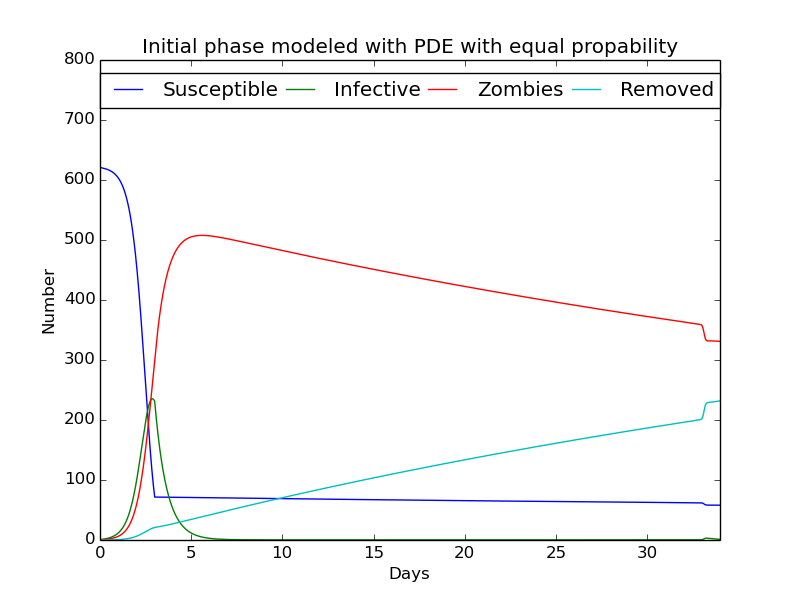
\includegraphics[width=0.8\linewidth]{2_fig/2D_zombie_three_phases_number.png}}
  \caption{
  \label{fig:zombie_three_number} The Eq.(\ref{eq:SIZR_disc2}) modeled with uniformed distributed groups. Initial values $S_0 = 621$, $I_0 = 0$, $Z_0 = 0$ and  $R_0 = 0$ with parameters from (\ref{table:param_val}).
  }
\end{figure}
%\clearpage % flush figures fig:zombie_three_number




\vspace{3mm}




\vspace{3mm}


The initial values for the four groups are set to $S_0=621$, $I_0=0$, $Z_0=1$ and $R_0= 0$ in all simulations. The values in Tab.(\ref{table:compare_phases_zombie}) are measured at the final time for each phase. The \emph{Initial phase} lasts for three days and the values are measured at $time=3$. The \emph{Hysterical phase} is a continuous phase, and will not stop until an eventual eradication. The values are therefore given before the \emph{Counter attack} at $time=33$. The \emph{Counter attack} lasts for some hours, and is measured at $time=34$, which is a day after the attack. The value of $\Delta t$ is set to 1E-3. 

\label{table:compare_phases_zombie}

\begin{quote}
\begin{tabular}{cccc}
\hline
\multicolumn{1}{c}{  } & \multicolumn{1}{c}{ ODE system } & \multicolumn{1}{c}{ PDE uniform dist } & \multicolumn{1}{c}{ PDE gauss center } \\
\hline
Initial phase    & ----------- & ------------------- & ------------------- \\
\hline
Susceptible      & 71.3        & 71.3                & 81.12               \\
Infected         & 230.8       & 230.8               & 210.94              \\
Zombie           & 298.9       & 298.9               & 310.11              \\
Removed          & 21.0        & 21.0                & 20.60               \\
\hline
Hysterical phase & ----------- & ------------------- & ------------------- \\
\hline
Susceptible      & 61.6        & 61.6                & 70.55               \\
Infected         & 0.3         & 0.3                 & 0.34                \\
Zombie           & 358.6       & 355.6               & 334.33              \\
Removed          & 201.5       & 201.5               & 217.56              \\
\hline
Counter attack   & ----------- & ------------------- & ------------------- \\
\hline
Susceptible      & 57.8        & 57.8                & 66.50               \\
Infected         & 1.2         & 1.2                 & 1.23                \\
Zombie           & 331.8       & 331.8               & 305.86              \\
Removed          & 231.3       & 231.3               & 249.19              \\
\hline
\end{tabular}
\end{quote}

\noindent
These results shows that the PDE system gives the same results as the ODE system.

% #
% #
% #
% #


\subsection{The position of the \emph{Infected} group}
In the previous section, \emph{English boarding school}, the location of the \emph{Infected} group was proven to have a major influence on the result. However here the \emph{Susceptible} group was uniformly distributed over the schoolyard. The number in each group, based on the study of \emph{Walking Dead}, was seen in three different locations in the TV series. By only studying the TV series, it is hard to decide the geographical distance between these three locations. Therefore they have been placed with a certain distance from each other. The following simulations are done on a grid with size(40 x 40) with the following positions for the towns: Small town(6,6) with size 21, middle town(12,25) with size 200 and large town(25,12) with size 400. Since these values were based on the humans and zombies seen in the series, these can be scaled up by 1000 to correspond a realistic population. A large town can be seen as an area with a population of 400 000. The length can be measured in kilometres. Then the distance between the middle and large town will be 18.38 km. Compared to the distance between Oslo and Bærum(Sandvika) which is 15 km, the simulation can be seen as a rough estimate of the area around Oslo, if the fjord is frozen and the mobility for the area is similar.


\vspace{3mm}




\vspace{3mm}


The diffusion term describes the diffusion for each group. This can be seen as the speed towards equilibrium for each group. If the diffusion constant is large, the flow towards equilibrium will go faster. The values have been set as follows. 
\begin{itemize}
\item $D_s=1$, The \emph{Susceptible} has a basic moving speed. The other groups are based on the speed of a healthy human.

\item $D_i=0.5$, The \emph{Infected} are often injured caused by recent fights. This affects their mobility.

\item $D_z=0.9$, The average moving speed for a zombie. There are zombies with the mobility of a human, but there are also zombies that drag themselves forward with only one arm. This results in a major difference in speed and therefore a lower average speed for the zombies.

\item $D_r=0$, The removed are here seen as dead, therefore there is no mobility.
\end{itemize}

\noindent


\vspace{3mm}




\vspace{3mm}


The parameters from Tab.(\ref{table:param_val}) will be used here, and the three phases will be modeled as shown for the uniformed distributed PDE system. The values will be used for three different simulations with the similar initial value for the different groups. The position of initial values can be seen in Fig.(\ref{fig:initial_value_susceptible}) and are based on the data given for each town above. The difference in the three simulations will be the position of the zombie at initial time. The zombie will be placed in center of the small, middle and large town.


\begin{figure}[ht]
  \centerline{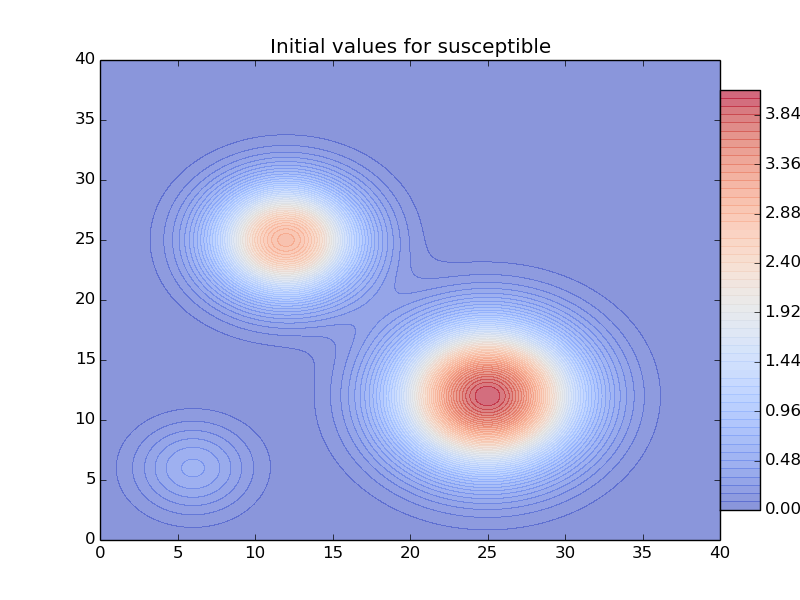
\includegraphics[width=0.8\linewidth]{2_fig/initial_value_susceptible.png}}
  \caption{
  \label{fig:initial_value_susceptible} The initial value for the \emph{Susceptible} group for three simulations. Small group(6,6) with volume 21, middle group(12,25) with volume 200 and large group(25,12) with volume 400. All three groups are build up with a Gaussian function.
  }
\end{figure}
%\clearpage % flush figures fig:initial_value_susceptible




\vspace{3mm}




\vspace{3mm}


Fig.(\ref{fig:large_town}) shows the simulation where the zombie is placed in the large town. The simulations of the small and middle town can be seen in the Appendix. The four subplots are from the different phases that arise during a zombie attack. The different groups have the same color as introduced in Fig.(\ref{fig:zombie_three_number}). It is difficult to separate the three groups \emph{Infected}, \emph{Zombie} and \emph{Removed}, since they all have a low value at initial time. The development of the amount can easier be seen in the Fig.(\ref{fig:compare_towns}), which also shows the results from the small and middle town. Since the amount of \emph{Susceptible} is quite low in the small town where the zombie arises, the disease is not able to infect too many before the society has moved to the next phase, assuming that the broadcasting about the disease works okay for the first days. This results in an eradication of the disease in about a month. The table(\ref{table:compare_phases_zombie}) shows that the number of zombies decreases towards zero after a month. 


\begin{figure}[ht]
  \centerline{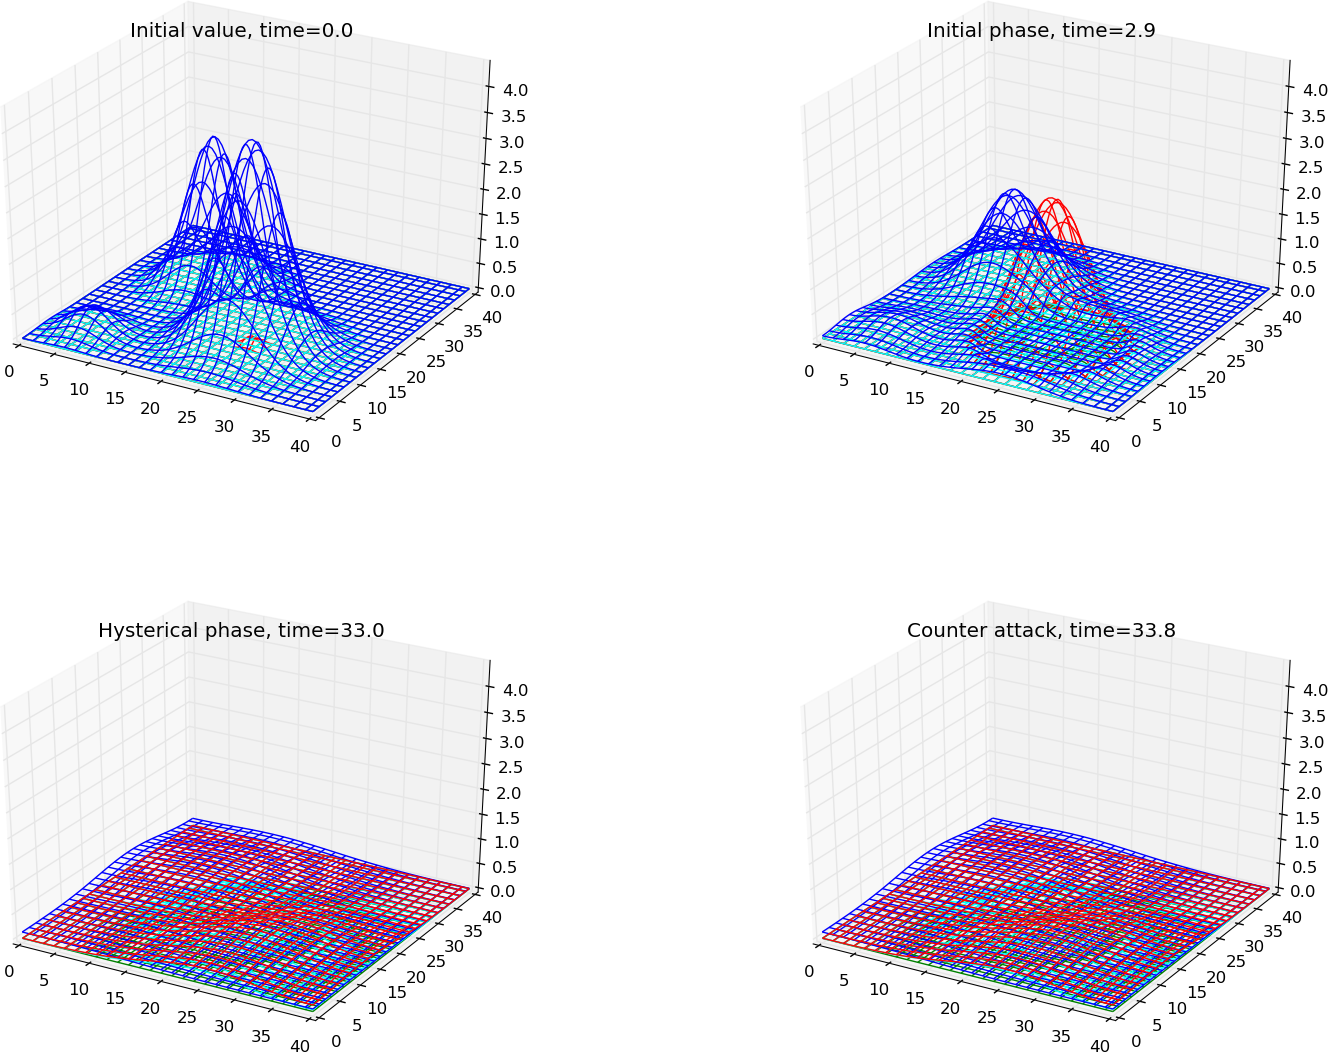
\includegraphics[width=0.8\linewidth]{2_fig/2D_zombie_three_phases_zombie_large_town_2_sub.png}}
  \caption{
  \label{fig:large_town} \emph{Walking Dead} simulated with the zombie at initial time in the large town. Subplots shown at each phase.
  }
\end{figure}
%\clearpage % flush figures fig:large_town




\vspace{3mm}




\vspace{3mm}


By placing the zombie in the middle town, the amount in the \emph{Zombie} group increases to a higher level. The amount can be seen as subplot II in Fig.(\ref{fig:compare_towns}). The damages are higher, and after a month the total population of \emph{Susceptible} is reduced to 427. The last calculation done for the large town in Fig.(\ref{fig:large_town}) shows major damages. Here the amount in the \emph{Zombie} group increases above the number of \emph{Susceptible}. The \emph{Infected} group also increases to above 100 after a couple of days in the initial phase. This can be explained by the high number of meetings between susceptible and zombies. By studying the subplot II in Fig.(\ref{fig:large_town}), the zombies are grouped in the large town, while the middle and small town mostly consist of \emph{Susceptible}. By counting the loss of \emph{Susceptible} during the first phase, the Tab.(\ref{table:compare_towns}) shows that this amount corresponds with the size of the towns where the zombie was placed, given by the number 17,188 and 362 in the small,middle and large group. The percent is highest in the middle town with 94 percent. The percent in the large and small group are 90 and 81.  The simulation in the middle town has the highest percent because the \emph{Susceptible} group in the large town also gets infected. These towns are coupled together, and the epidemic disease is able to spread. The small town, which can be seen as Nesodden(a peninsula outside Oslo), has the lowest percent. The reason is that the disease is not able to spread to the other towns, and therefore is causes less damage.  


\begin{figure}[ht]
  \centerline{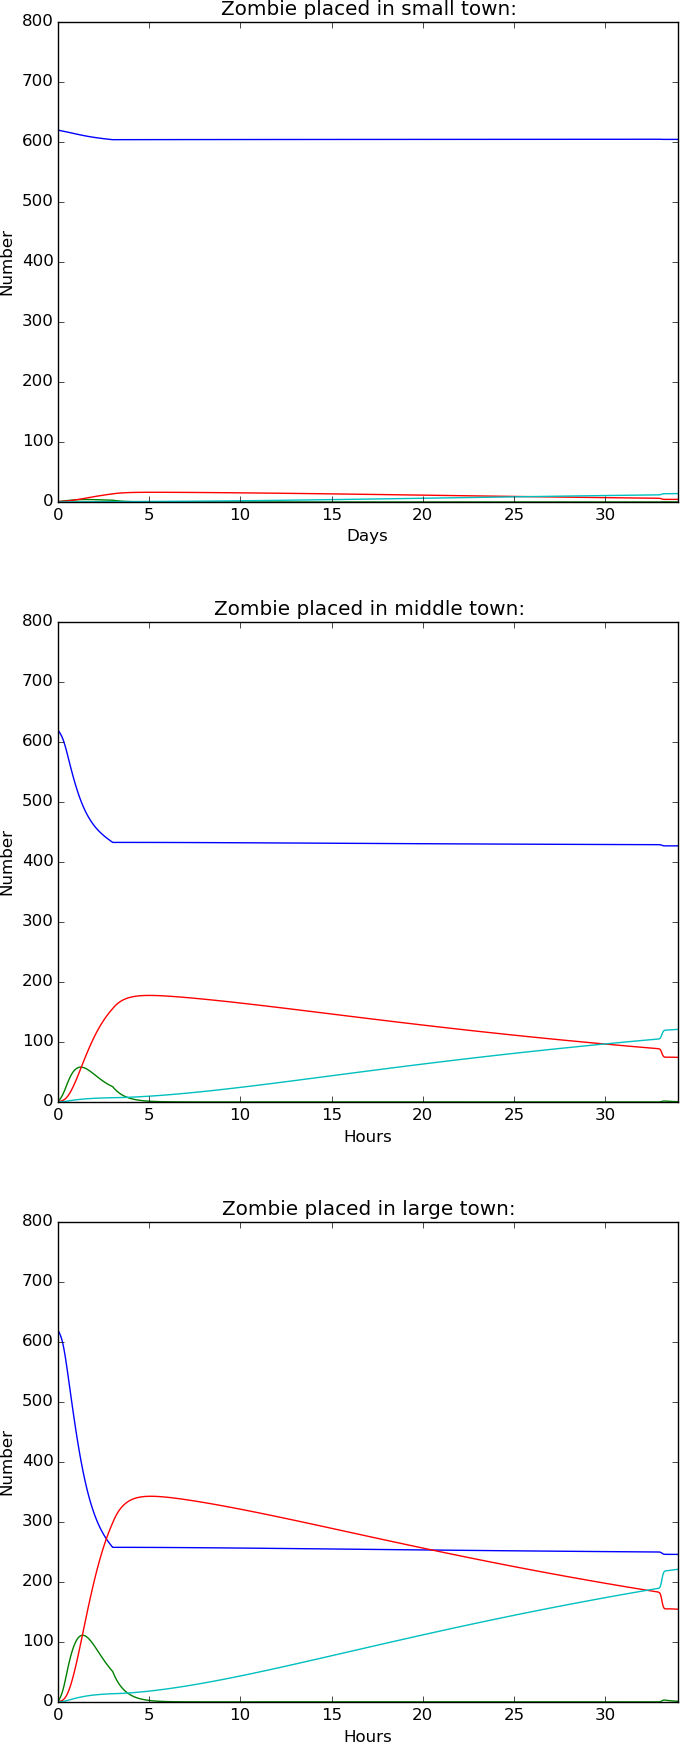
\includegraphics[width=0.6\linewidth]{2_fig/2D_compare_towns.png}}
  \caption{
  \label{fig:compare_towns} The values for each group counted during 34 days in \emph{Walking Dead}. Initial phase from day 0 to day 3, Hysterical phase from day 3 to day 33 and Counter attack from day 33 to day 34.
  }
\end{figure}
%\clearpage % flush figures fig:compare_towns




\vspace{3mm}




\vspace{3mm}


The results from the uniformed distributed simulation is still much higher for the \emph{Zombie} group the in these three simulations. This shows that using the parameters from the ODE system in a geographical area makes little sense. A realistic assumption is that a zombie is restricted to a given area, and therefore the parameters will not be equal for all. The chance of getting infected is much higher if a person from the  \emph{Susceptible} group is close to an infected. There is also a greater chance of getting infected if the \emph{Susceptible} group has a high density. 

% FIGURE:[2_fig/2D_zombie_three_phases_zombie_small_town_2_number.png, height=600 width=800 frac=0.8]

% FIGURE:[plots/2D_zombie_three_phases_zombie_middle_town_2_number.png, height=600 width=800 frac=0.8]

% FIGURE:[plots/2D_zombie_three_phases_zombie_large_town_2_number.png, height=600 width=800 frac=0.8]





\label{table:compare_towns}

\begin{quote}
\begin{tabular}{cccc}
\hline
\multicolumn{1}{c}{  } & \multicolumn{1}{c}{ Small town } & \multicolumn{1}{c}{ Middle town } & \multicolumn{1}{c}{ Large } \\
\hline
Initial phase    & ----------- & ------------------- & ------------------- \\
\hline
Susceptible      & 603.74      & 433.22              & 259.20              \\
Infected         & 2.96        & 25.51               & 50.94               \\
Zombie           & 13.79       & 155.27              & 297.24              \\
Removed          & 0.66        & 7.16                & 13.78               \\
\hline
Hysterical phase & ----------- & ------------------- & ------------------- \\
\hline
Susceptible      & 604.42      & 429.35              & 251.14              \\
Infected         & 0.03        & 0.18                & 0.35                \\
Zombie           & 6.25        & 87.31               & 178.45              \\
Removed          & 12.14       & 106.00              & 192.90              \\
\hline
Counter attack   & ----------- & ------------------- & ------------------- \\
\hline
Susceptible      & 604.21      & 427.45              & 247.33              \\
Infected         & 0.08        & 0.59                & 1.17                \\
Zombie           & 4.49        & 73.70               & 151.44              \\
Removed          & 14.11       & 121.16              & 222.96              \\
\hline
\end{tabular}
\end{quote}

\noindent
\subsection{Free areas for the \emph{Susceptible} group}
To model a realistic zombie attack, humans ability to think logically is crucial in the fight. The mobility was presented as a factor in the previous section. Another important skill that the \emph{Susceptible} group holds, is the ability to decide the safety of an area. In the TV series \emph{Walking Dead}, the humans build barricades to keep the zombies outside. This gives the \emph{Susceptible} group free areas where they can stay. This idea can be transfered to the PDE system by rewriting the Eq.(\ref{eq:seland_model_PDE}) with spatial dependent diffusion terms. The diffusion constant $D_u$ is now replaced with a diffusion function $\gamma_u(x)$ for $u= S,I,Z,R$, which is spatial discretized. Since a diffusion equation always goes towards equilibrium, this rewriting will only slow down/stop the selected group to diffuse into an area. In this case it will stop the \emph{Zombie} group from diffusing into the buildings. 
\begin{equation} \label{eq:seland_model_diff}
    \begin{aligned} 
    \frac{\partial S}{\partial t} =& \Sigma -(\beta+\mu \omega(t))SZ - \delta_SS +\nabla(\gamma_S(x) \nabla S) \\
    \frac{\partial I}{\partial t} =& (\beta+\mu \omega(t))SZ - \varrho I - D_i\delta_II+\nabla(\gamma_I(x) \nabla I)\\
    \frac{\partial Z}{\partial t} =& \varrho I- (\alpha+\omega(t))SZ + \zeta R+\nabla(\gamma_Z(x) \nabla Z)\\
    \frac{\partial R}{\partial t} =& \delta_SS +\delta_II -\zeta R + (\alpha+\omega(t))SZ+\nabla(\gamma_R(x) \nabla R) 
    \end{aligned}
\end{equation}
The diffusion term is the difference between this system and Eq.(\ref{eq:seland_model_PDE}). The discretization can be shown for for a general $\gamma$. This will be similar for all groups. A centered difference is used in space.
\begin{equation} \label{eq:gamma}
    \begin{aligned}
    &=\nabla(\gamma(x) \nabla S) \\
    &=(\gamma(x) S_x)_x+(\gamma(x) S_y)_y \\
    &= \left(\gamma(x) \frac{S^{n}_{i+1/2,j}-S^{n}_{i-1/2,j}}{\Delta x}\right)_x+\left(\gamma(x) \frac{S^{n}_{i,j+1/2}-S^{n}_{i,j-1/2}}{\Delta y}\right)_y \\
    &= \left(\frac{\gamma(x_{i+1/2,j})(S^{n}_{i+1,j}-S^{n}_{i,j})-\gamma(x_{i-1/2,j})(S^{n}_{i,j}-S^{n}_{i-1,j})}{\Delta x^2}\right) \\
    &+ \left(\frac{\gamma(x_{i,j+1/2})(S^{n}_{i,j+1}-S^{n}_{i,j})-\gamma(x_{i,j-1/2})(S^{n}_{i,j}-S^{n}_{i,j-})}{\Delta y^2}\right)
    \end{aligned}
\end{equation}
Since the calculations are based on spatial points, the values inside the function of $\gamma$ need to be adjusted. This can be done by the use of an arithmetic mean, which can be seen in Eq.(\ref{eq:arith_mean}). The notation $q_{i+1/2}$ is a simplification of the function $q(x_{i+1/2})$ with $x_{i+1/2} = x_i + 1/2 \Delta x$
\begin{equation} \label{eq:arith_mean}
q_{i+1/2} \approx \frac{1}{2}(q_i +q_{i+1})
\end{equation}
This arithmetic mean can be inserted for all $\gamma$'s in the system. The system can be expressed:
\begin{equation} \label{eq:SIZR_disc3}
	\begin{aligned}
    S^{n+1}_{i,j}   &= S^n_{i,j} + \Delta t \Bigl( \Sigma - (\beta+\mu \omega(t))S^{n}_{i,j}Z^{n}_{i,j}- \delta_S S^{n}_{i,j} \\
                    &+ \frac{1}{2\Delta x^2}\left(\gamma_S(x_{i-1,j})(S^{n}_{i-1,j}-S^{n}_{i,j})+\gamma_S(x_{i,j})(S^{n}_{i-1,j}-2S^{n}_{i,j}+S^{n}_{i+1,j})+\gamma_S(x_{i+1,j})(-S^{n}_{i,j}+S^{n}_{i+1,j})\right) \\
                    &+ \frac{1}{2\Delta y^2}\left(\gamma_S(x_{i,j-1})(S^{n}_{i,j-1}-S^{n}_{i,j})+\gamma_S(x_{i,j})(S^{n}_{i,j-1}-2S^{n}_{i,j}+S^{n}_{i,j+1})+\gamma_S(x_{i,j+1})(-S^{n}_{i,j}+S^{n}_{i,j+1})\right)\Bigr)\\
    I^{n+1}_{i,j}   &= I^n_{i,j} + \Delta t \Bigl((\beta+\mu \omega(t))S^{n}_{i,j}Z^{n}_{i,j}-\varrho I^{n}_{i,j}- \delta_I I^{n}_{i,j} \\
                    &+ \frac{1}{2\Delta x^2}\left(\gamma_I(x_{i-1,j})(I^{n}_{i-1,j}-I^{n}_{i,j})+\gamma_I(x_{i,j})(I^{n}_{i-1,j}-2I^{n}_{i,j}+I^{n}_{i+1,j})+\gamma_I(x_{i+1,j})(-I^{n}_{i,j}+I^{n}_{i+1,j})\right) \\
                    &+ \frac{1}{2\Delta y^2}\left(\gamma_I(x_{i,j-1})(I^{n}_{i,j-1}-I^{n}_{i,j})+\gamma_I(x_{i,j})(I^{n}_{i,j-1}-2I^{n}_{i,j}+I^{n}_{i,j+1})+\gamma_I(x_{i,j+1})(-I^{n}_{i,j}+I^{n}_{i,j+1})\right)\Bigr)\\
    Z^{n+1}_{i,j}   &= Z^n_{i,j} +\Delta t \Bigl( \varrho I^{n}_{i,j}-(\alpha+\omega(t))S^{n}_{i,j}Z^{n}_{i,j}+ \zeta R^{n}_{i,j} \\
                    &+ \frac{1}{2\Delta x^2}\left(\gamma_Z(x_{i-1,j})(Z^{n}_{i-1,j}-Z^{n}_{i,j})+\gamma_Z(x_{i,j})(Z^{n}_{i-1,j}-2Z^{n}_{i,j}+Z^{n}_{i+1,j})+\gamma_Z(x_{i+1,j})(-Z^{n}_{i,j}+Z^{n}_{i+1,j})\right) \\
                    &+ \frac{1}{2\Delta y^2}\left(\gamma_Z(x_{i,j-1})(Z^{n}_{i,j-1}-Z^{n}_{i,j})+\gamma_Z(x_{i,j})(Z^{n}_{i,j-1}-2Z^{n}_{i,j}+Z^{n}_{i,j+1})+\gamma_Z(x_{i,j+1})(-Z^{n}_{i,j}+Z^{n}_{i,j+1})\right)\Bigr)\\
    R^{n+1}_{i,j}   &= R^n_{i,j} +\Delta t \left(\delta_S S^{n}_{i,j}+\delta_I I^{n}_{i,j}-\zeta R^{n}_{i,j}+(\alpha+\omega(t))S^{n}_{i,j}Z^{n}_{i,j}\right)
	\end{aligned}
\end{equation}
The diffusion term for the \emph{Removed} group is taken away, since dead people are not able to move. This system looks quite messy, but it is straight forward to calculate. All values on the right side are known values and the system is easy to solve. Now every point will be controlled by the diffusion constants given in $\gamma(x)$. This makes it easier to control the flow in each group. With a high diffusion constant, the diffusion will spread fast. When the diffusion constant goes towards zero, the flow will decrease towards zero flow. This will result in a set of ODE systems modeled for each point.

\subsection{Ten minutes at Frederikkeplassen}
Frederikkeplassen at the University of Oslo is a possible area for an upcoming zombie attack. This simulation will try to model a ten minute sequence with the diffusion parameter added in this section. Since students often learn and interact fast, they will only use three minutes before they realize the danger and transitions into the \emph{Hysterical phase}. A map of Frederikkeplassen is used to define the safe and critical areas. The buildings are set as areas where only the \emph{Susceptible} are allowed to move. This is done by setting the diffusion constant to zero for the \emph{Zombie} and \emph{Infected} groups. Since the buildings are safe spots for the \emph{Susceptible}, an idea would be to express this in the diffusion term by forcing the \emph{Susceptible} for other areas into the buildings. This is more difficult, since the concentrations in each group wants to diffuse towards equilibrium. A way to delay this process is by setting the diffusion constant to be low in the buildings and high outside. This will result in a fast diffusion in the open areas and a slow diffusion inside the buildings. 


\begin{figure}[ht]
  \centerline{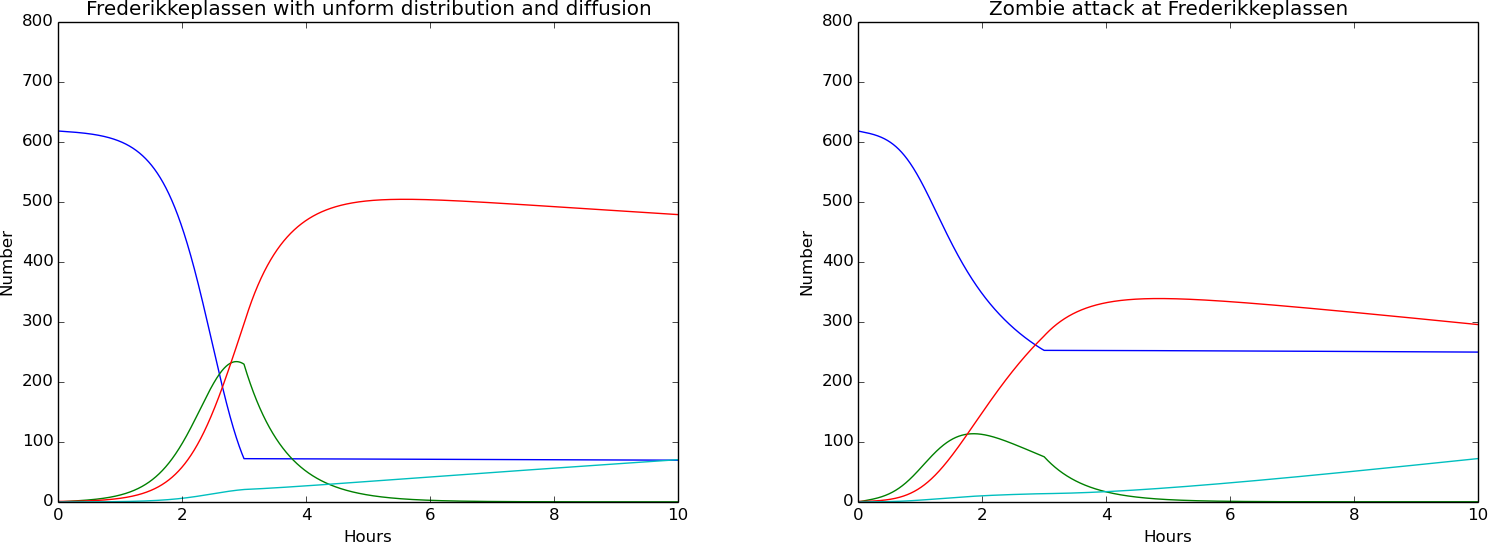
\includegraphics[width=0.8\linewidth]{2_fig/2D_compare_Frederikke.png}}
  \caption{
  \label{fig:frederikke_numbers} The amount in each group for two simulations of Frederikkeplassen modeled same parameters for 10 minutes/hours. a)Plot with uniformed distributed groups and same diffusion constants for all groups. b)Plot based on figure(\ref{fig:frederikke_free_area}) with different initial values for each group.
  }
\end{figure}
%\clearpage % flush figures fig:frederikke_numbers




\vspace{3mm}




\vspace{3mm}


Two simulations have been done at Frederikkeplassen. The amount in each group can be seen in Fig.(\ref{fig:frederikke_numbers}). The first simulation has a solution based on the ODE system, with uniformed distributed groups, equal diffusion constants and no free areas for the \emph{Susceptible}. The second simulation is modeled with three groups of \emph{Susceptible}, as in the previous section. The small group with 21 students is placed at point(4,4), the middle group with 200 students is placed at point(15,8) and the large group with 400 students is placed at point(8,13). The zombie is placed at point(8,10). The $\gamma(x)$ is set to zero in the buildings for the \emph{Zombie} and \emph{Infected} group, and one in the rest of the area. For the \emph{Susceptible} group, $\gamma(x)$ is set to 0.1 in the buildings, which causes slow diffusion. In the outside areas, $\gamma(x)$ is set to 5 for the \emph{Susceptible}. The desired result is to push them into the buildings, but this will only happen if there is a lower concentration inside the buildings. Therefore this will not reflect a realistic flow of a \emph{Susceptible} population. This simulation can be seen in Fig.(\ref{fig:frederikke_free_area})  


\begin{figure}[ht]
  \centerline{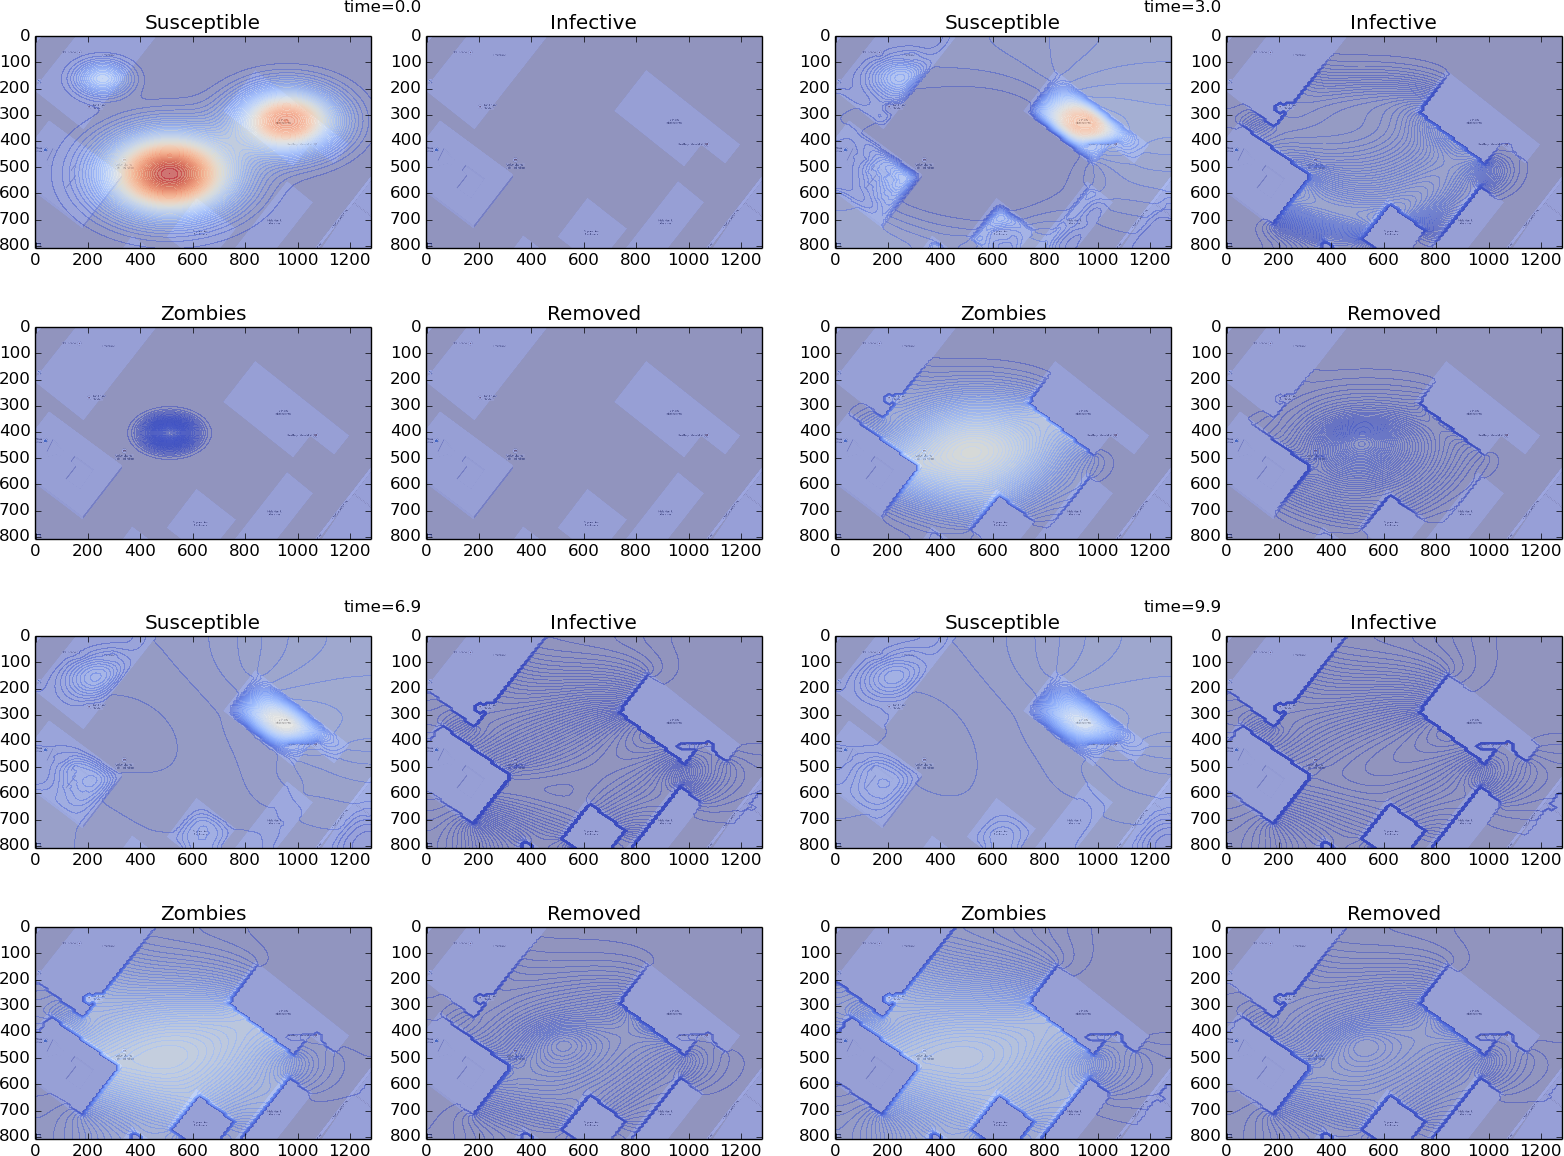
\includegraphics[width=0.8\linewidth]{2_fig/2D_Frederikke_contourf_sub.png}}
  \caption{
  \label{fig:frederikke_free_area} Frederikkeplassen modeled with free areas for the \emph{Susceptible} group. The diffusion function $\gamma(x)$ is set to zero for the \emph{Zombie} and \emph{Infected} group in the buildings. The zombie at initial time is placed in the center of Frederikkeplassen
  }
\end{figure}
%\clearpage % flush figures fig:frederikke_free_area




\vspace{3mm}




\vspace{3mm}


The results in Tab.(\ref{table:frederikke_table}) shows that the three first minutes are crucial. The number after three minutes shows that only 72 humans survived the attack in the uniformed solution, compared to 252 in the free areas. The number in the \emph{Zombie} group is quite similar in \emph{Uniformed distribution} and \emph{Free areas} measured at $t=3$. However at $t=7$ the difference is major. This can be explained by looking at Fig.(\ref{fig:frederikke_free_area}) and the building with the middle group placed inside. When the zombie starts attacking at $t=0$, the large group is exposed. This group is placed close to the zombie and the position is in an open area. The zombie can attack right away and the number in the \emph{Infected} and \emph{Zombie} groups increases fast. In the two first minutes, a major part of the large group is infected and the \emph{Zombie} group starts to spread. After 2-3 minutes, the group has reached the buildings with the middle group. Here the diffusion is set to 0, and the spread of zombies stop. Since the diffusion variable for the \emph{Susceptible} is quite low inside the buildings, it takes time before the group diffuses. Maybe the right diffusion value along the buildings would be 0, to avoid any leakage. This would again cause problem for the diffusion of \emph{Susceptible} into the buildings. It is also reasonable to think that the \emph{Susceptible} group needs to diffuse after a certain time. The lack of supplies would force them out.

\label{table:frederikke_table}

\begin{quote}
\begin{tabular}{ccc}
\hline
\multicolumn{1}{c}{  } & \multicolumn{1}{c}{ Uniform distribution } & \multicolumn{1}{c}{ Free areas } \\
\hline
3 Minutes   & --------------------------- & --------------- \\
\hline
Susceptible & 72.23                       & 252.72          \\
Infected    & 229.65                      & 75.69           \\
Zombie      & 296.67                      & 276.55          \\
Removed     & 20.84                       & 13.94           \\
\hline
7 Minutes   & --------------------------- & --------------- \\
\hline
Susceptible & 70.78                       & 251.35          \\
Infected    & 0.83                        & 0.51            \\
Zombie      & 498.72                      & 325.54          \\
Removed     & 49.12                       & 41.26           \\
\hline
10 Minutes  & --------------------------- & --------------- \\
\hline
Susceptible & 69.69                       & 249.84          \\
Infected    & 0.25                        & 0.38            \\
Zombie      & 479.00                      & 295.71          \\
Removed     & 70.55                       & 72.36           \\
\hline
\end{tabular}
\end{quote}

\noindent

\section{Discussion}
This chapter expand the study of the disease, by adding the opportunity to analyse the disease for a spatial area. The travelling wave is essential for a disease to spread in an area. If the reproduction rate seen in Eq.(\ref{eq:reproduction_rate_PDF}) was below 1, the travelling wave would decrease towars zero and the disease would dissapear. By varying $\lambda$, one could see that a low value would cause a total eradication of the \emph{Susceptible}. By setting $\lambda>=1$, the damage from the epidemic wave would be close to zero and the disease would die out.


\vspace{3mm}




\vspace{3mm}


The results from the English boarding school shows that the position of the infected student has a major impact on the result. A uniform distribution was first calculated and compared with the ODE simulation in the previous chapter. This gave the same result. By varying the position of the infected student, the result was affected. When simulating the disease for a long time, the number of \emph{Infected} students seems to be similar. Therefore the parameter values in the system will not be enough to say anything about the concentrations measured in time for each group. The position will also affect the result. 


\vspace{3mm}




\vspace{3mm}


The section \emph{Zombiefication} verified the uniform distribued PDF solution with the ODE solution from the previous chapter. These were expected to be similar. The English boarding school studied the result of varying the position of the infected with a uniform distributed group of \emph{Susceptible}. This section tried to expand this idea byspread the group of \emph{Susceptible} into three groups. The position of the zombie was placed in center of all three groups. The amount of \emph{Infected} in these three simulations was proportional to the size of the group where the zombie was placed. The position of the infected student was shown to have an impact on the spread of the disease. This section shows that the \emph{Susceptible} group also affects the result.


\vspace{3mm}




\vspace{3mm}


The last part \emph{Ten minutes at Frederikke} tries to implement human behavior by giving the \emph{Susceptible} group the ability to keep zombies outside the buildings. This was crucial in \emph{Walking Dead} to prevent meetings between zombies and humans. One can see from the results that this gives the \emph{Susceptible} group a greater chance of surviving. The concentrations for each group will go towards equilibrium. Therefore this simulation will differ from human behavior. The next chapter will use random walks to simulate this zombie outburst. This will build on \emph{Ten minutes ad Frederikke}, and introduce different conditions based on the phase the zombies and humans are in. 



\chapter{Random walk}
The last chapter will study a third way to model epidemic diseases. This will be done by using random walk. This technique is quite different from the two models presented earlier. Here Monte Carlo simulations and probabilities are used instead of differential equations, which have been in focus earlier. The first section will be an introduction to general principles for Monte Carlo methods and Random walk based on the paper from M.H. Jensen Ref.\cite{hjorth2011computational}. The next sections will use the parameters from the \emph{English Boarding School} and \emph{Walking Dead} to see if a random walk system can expand the knowledge about epidemics by adding human behavior. 

\section{Monte Carlo methods}
\label{sec:monte_carlo_methods}
Techniques from Monte Carlo are widely used in several fields as chemistry, physics, medicine, biology and in finance Ref. \cite{hjorth2011computational}. These numerical methods can be seen in general terms as statistical simulation methods, which use random numbers to perform the simulations. Four terms are required to understand the Monte Carlo strategy:
\begin{itemize}
\item Random variable

\item Probability distribution functions (PDF)

\item Moments of a PDE

\item The pertinent variance $\sigma ^2$
\end{itemize}

\noindent
The two first terms are important when modelling a random walk simulation, while the two last terms are important when studying the result. The four terms are explained below.

\subsection{Random variable}
Random variable can be seen as a stochastic variable, where the outcome cannot be presumed. Examples as tossing dice, flipping coins or gambling are based on this principle. Although the outcome is unknown, knowledge about the probability and the range can be studied. The numbers in the \emph{domain} for two dice are
\begin{equation*}
\{2,3,4,5,6,7,8,9,10,11,12\}
\end{equation*}
with the corresponding \emph{probabilities} are
\begin{equation*}
\{1,2,3,4,5,6,5,4,3,2,1\}\frac{1}{36}
\end{equation*}
By throwing two dice once, there is no guarantee that the result will be 7, though this has the highest probability. However, by repeating this operation, the distribution would reflect the \emph{probabilities} above. A stochastic variable can either be discrete or continuous, but will in both cases be denoted as capital letters, $X,Y$. A discrete example is the example above, where the domain is given with exact values, ${x_1,x_2,x_3,...,x_n}$. The continuous case can be seen as the probability in a given area. An example can be the distance from a dart to the center, after trowing a dart randomly.


\vspace{3mm}




\vspace{3mm}


This chapter will use random variable for several decisions. The path of the walker will be controlled by two random variables. The first will control the direction of the walker, by drawing a random number between $0$ and $2\pi$. The second random variable will control the number of time steps walked in the chosen direction. Here a number between 1 and 20 is drawn. This is done to create a more realistic movement pattern. Random variables will be drawn for each parameter value given in the previous ODE and PDE systems. Here the outcome will be based on the random variable and the probability given by the parameter value. 

\subsection{Probability distribution functions (PDF)}
The PDF is a function $p(x)$ on the domain that gives the probability or relative frequency for a outcome. In the discrete case, the function can be seen as
\begin{equation}
p(x) = Prob(X=x)
\end{equation}
The PDF in the continuous case is not able to directly depict the actual probability. The probability is instead defined as the density around $x$ with an infinitesimal interval. This can therefore be seen as an integral, since it is the density of the probability rather than the probability Ref.\cite{hjorth2011computational}. This can be defined.
\begin{equation}
 Prob(a\leq X \leq b) = \int^b_a p(x)dx
\end{equation}
To quote M.H. Jensen "Qualitatively speaking, a stochastic variable represents the values of numbers chosen as if by chance from some specified PDF so that the selection of a large set of these numbers reproduces this PDF." Ref.\cite{hjorth2011computational}. This sums up the relation between random variables and the PDF. If this is not fulfilled, the group of stochastic variables does not fulfill the criteria for random numbers. 

There are two properties that the PDF must fulfill. The first one is the size of $p(x)$. This has to be in the interval $0\leq p(x) \leq 1$, since the probability cannot be negative or larger than 1 for an event to happen. The sum of all events has to be 1, both for discrete and continuous PDFs, and can be seen as follows
\begin{equation}
	\begin{aligned}
    \sum_{x_i \in \mathbb{D}} p(x_i) = 1\\
    \int_{x \in \mathbb{D}} p(x) dx = 1
	\end{aligned}
\end{equation} 

There are several distributions that are essential when looking at continuous PDFs. The main PDF in this chapter will be uniform distribution and can be seen in Eq.(\ref{eq:uni_dist}).
\begin{equation} \label{eq:uni_dist}
p(x) = \frac{1}{b-a}\theta(x-a)\theta(b-x)
\end{equation}
with:
\begin{equation}
	\begin{aligned}
    \theta(x) = 0,\quad x < 0 \\
    \theta(x) = 1,\quad x \geq 0
	\end{aligned}
\end{equation}
This is used to disperse the group of walkers at initial time over the area. The chance will be equal for all positions. This PDF is also used in the movement pattern and for the spread of the disease. To get a correct estimate, it is important that the set of random numbers is large enough. Gaussian distribution is the second PDF used in this chapter. This is often called normal distribution and can be seen in Eq.(\ref{eq:gauss_dist})
\begin{equation} \label{eq:gauss_dist}
	\begin{aligned}
    p(x) = \frac{1}{\sigma \sqrt{2\pi}} \exp(-\frac{(x-\mu)^2}{2\sigma^2})
	\end{aligned}
\end{equation}
This will give the same distribution as the Gaussian function used in the previous chapter. Here it will be used for the simulations of all three phases, to describe the initial positions of the walkers. 

\subsection{Moments of a PDF}
By defining $h(x)$ as an arbitrary function, the \emph{expectation value} can be written
\begin{equation}
    \langle h \rangle_X \equiv \int h(x)p(x)dx
\end{equation}
Here, defined on the domain of the stochastic variable $X$, with PDE $p(x)$. A more general way to write the expectation is by adding a power of, $n$, to the equation. This can now be seen as the \emph{moments}. The $n$-th moment is defined
\begin{equation}
    \langle x^n \rangle \equiv \int x^np(x)dx
\end{equation}
The value of $n$ can be set to zero. This results in $\langle 1 \rangle$ and creates a normalized condition for $p$. The first order is called \emph{mean} and is often defined with a $\mu$.
\begin{equation}
    \langle x \rangle = \mu \equiv \int xp(x)dx
\end{equation}
This represents the average value of PDF and is often called the expectation value of $p$ Ref.\cite{hjorth2011computational}. Since this system consists of small group of walkers, which is modeled over a short period, the results from the simulations will vary. Therefore a set of simulations will be performed and the average values will be used. 
\subsection{The pertinent variance $\sigma ^2$}
\emph{Central moments} is a special case of moments defined as
\begin{equation}
    \langle (x-\langle x \rangle)^n \rangle \equiv \int (x-\langle x \rangle)^np(x)dx
\end{equation}
The first two central-moments are trivial and only result in 1 and 0, respectively for $n=0$ and $n=1$. However, the second central-moment is more interesting to study. This is denoted as $\sigma^2_X$ or Var(X), called the variance. This can be shown.
\begin{equation}
    \sigma^2_X  = \langle x^2\rangle -\langle x \rangle^2 
\end{equation}
The square root of the variance, $\sigma = \sqrt{\langle (x-\langle x \rangle)^2 \rangle}$ is called \emph{standard deviation}. This can be seen as the spread around the mean of the PDF. Since the result is based on the average value of a set of simulations, the \emph{standard deviation} also gives essential information. If the \emph{standard deviation} is major, one can expect large variations when modelling a system. This will make it more difficult to predict the result of an outcome. Since these systems are quite small, one can expect major variations and a large \emph{standard deviation}. 

\section{Random walker}
Now a random walker can be introduced in 1D. This can either jump to the left or to the right with a lenght of $\Delta x = l$. It is an equal probability for both directions. $L=R=1/2$. Then the average displacement will be 
\begin{equation}
 \langle x(n) \rangle = \sum^n_i \Delta x_i = 0, \quad \Delta x_i = \pm l,
\end{equation}
after $n$ jumps. The variance can be found by first finding $\langle x(n)^2 \rangle$.
\begin{equation}
\langle x(n)^2 \rangle = \left(\sum^n_i \Delta x_i\right)\left(\sum^n_j \Delta x_j\right) = \sum^n_i \Delta x_i^2 + \sum^n_i \Delta x_i \Delta x_j = l^2n
\end{equation}
The last term here will disappear after enough steps.  
\begin{equation}
\sum^n_i \Delta x_i \Delta x_j = 0
\end{equation}
This gives the variance
\begin{equation}
\langle x(n)^2 \rangle-\langle x(n) \rangle^2 = l^2n
\end{equation}
Now this variance from a random walker can be coupled with the variance from a diffusion equation. The variance from a diffusion equation is shown in the Appendix. By setting $n = t/\Delta t$. The random walker gets the following variance
\begin{equation}
\langle x(n)^2 \rangle-\langle x(n) \rangle^2 = l^2\frac{t}{\Delta t}
\end{equation}
Then the diffusion constant in the diffusion equation can be replaced with
\begin{equation}
D = \frac{l^2}{\Delta t}
\end{equation}
The variances between these two can be compared.


\begin{figure}[ht]
  \centerline{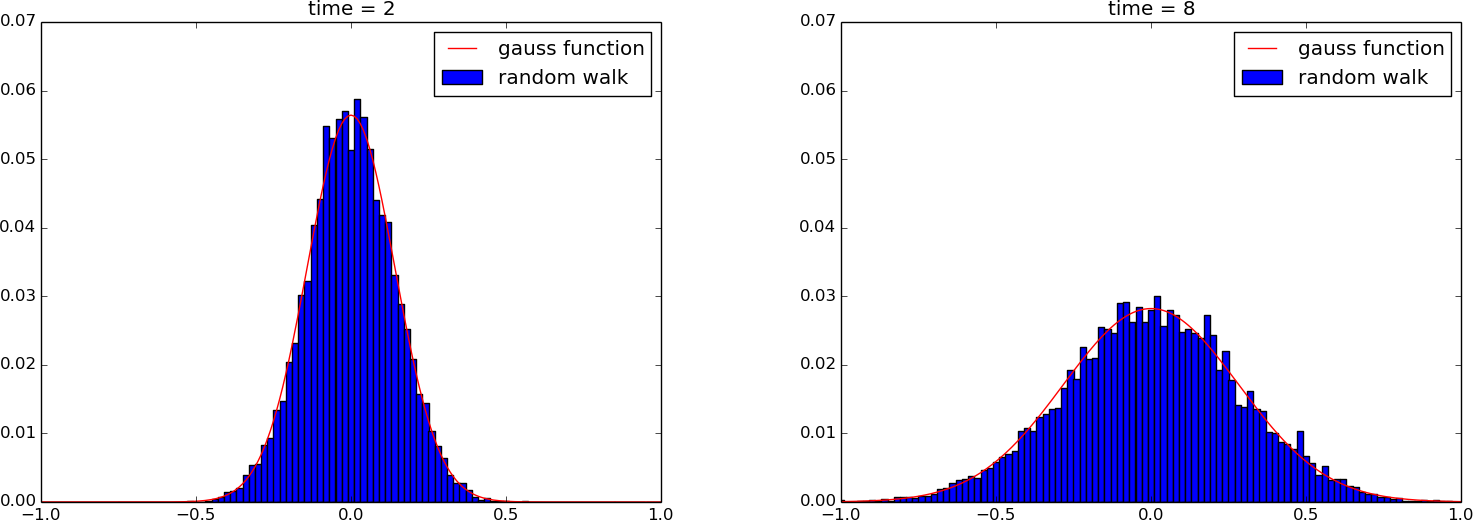
\includegraphics[width=1.0\linewidth]{3_fig/random_compare.png}}
  \caption{
  \label{fig:gauss_random} 10000 random walkers placed at x=0 at t=0. Every step has the length $\Delta x = 0.01$ and with a random step every $\Delta t = 0.01$.
  }
\end{figure}
%\clearpage % flush figures fig:gauss_random


The standard deviation can be found for this simulation. This is given by the square root of the variance
\begin{equation}
\sigma = \sqrt{l^2\frac{t}{\Delta t}}
\end{equation}

To study whether the average random walker develops as expected, a table with the outputs can be added. 

\label{table:gauss_random}

\begin{quote}
\begin{tabular}{ccc}
\hline
\multicolumn{1}{c}{  } & \multicolumn{1}{c}{ time=2 } & \multicolumn{1}{c}{ time=8 } \\
\hline
average displacement   & 0.000662 & -0.002416 \\
standard deviation(SD) & 0.1414   & 0.2828    \\
percent inside SD      & 70.96    & 69.02     \\
percent inside gauss   & 68.26    & 68.26     \\
\hline
\end{tabular}
\end{quote}

\noindent
The average displacement and the standard deviation shows that a group of random walkes spread similarly as a standard diffusion function. This result in a major group of random walkers. In the simulation in Fig.(\ref{fig:gauss_random}), 10000 random walkers are used. By increasing the amount om random walkers, the precision will be better.

\section{English Boarding School}
This example has been similar for all three systems, and will be used in this chapter. The chance of getting infected by influenza requires a meeting between an infected person and a susceptible person. A random walker will after a sufficient number of steps cover the whole area. A simulation is done for a student with a random position at initial time. 1000 random steps are taken every day, which results in a step every 90 seconds. The step length is set to 5.7024 m, and is based on the average distance a person walks every day. The simulation is performed for 15 days, which results in 15000 random steps. The size of the schoolyard is set to 100 m x 100 m, and the disease can spread within a distance of 5 meters.


\begin{figure}[ht]
  \centerline{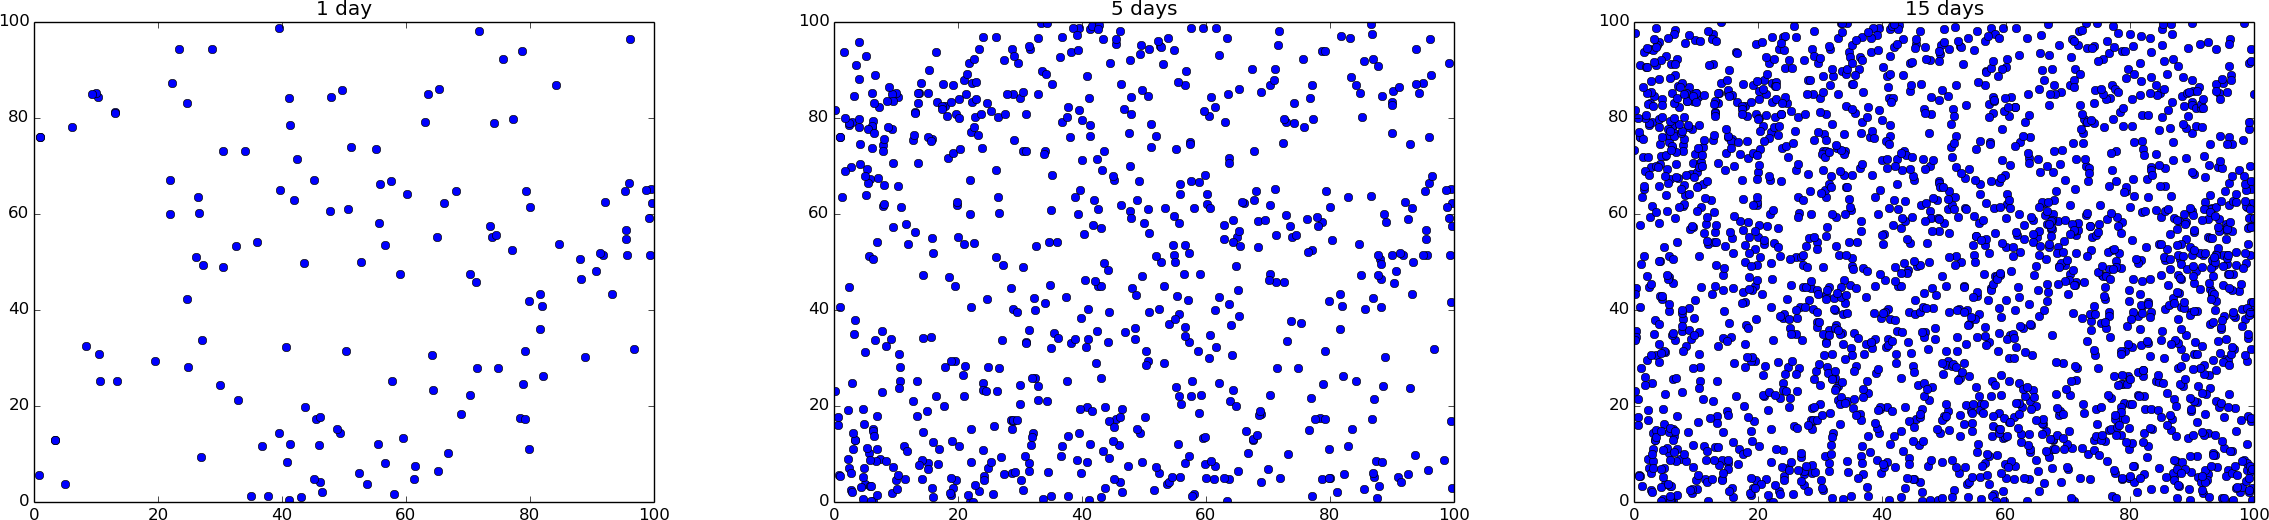
\includegraphics[width=0.8\linewidth]{3_fig/random_walk_days.png}}
  \caption{
  \label{fig:random_walker_days} The positions a random walker has covered in 1,5 and 15 days. A random step with length 5.7024 m is performed every minute. The positions are plotted for every ten minutes.
  }
\end{figure}
%\clearpage % flush figures fig:random_walker_days


Fig.(\ref{fig:random_walker_days}) shows that a random walker will be distributed over the area after enough steps. The students in the school are divided into three groups. 
\begin{itemize}
\item The \emph{Susceptible} group: This group consists of susceptible students, and this group is at risk of getting infected. This group is described by $S$. 

\item The \emph{Infected} group: This group consists of infected students. The group is described by $I$. 

\item The \emph{Removed} group: This group consists of students who are immune to the disease. This group is described by $R$. 
\end{itemize}

\noindent
The total number of students is $N=763$. The initial values are: $S_0=762$, $I_0=1$ and $R_0=0$. There are two parameters that are used in the simulation. The first parameter $r$, describes the gain of infected students from the \emph{Susceptible} group. This rate is proportional to the number of susceptible and infected students and is given by $rSI$. The second parameter $a$ describes the rate of removal from the \emph{Infected} group to the \emph{Removed} group. These two parameters are set to $r=2.18\cdot 10^{-3}$ and $a=0.44036$ for the ODE system simulated in section~\ref{section:ODE_models}. The ODE system can be seen in Eq.(\ref{eq:SIR_model_random})
\begin{equation} \label{eq:SIR_model_random}
	\begin{aligned} 
	\frac{dS}{dt} &= -rSI \\ 
	\frac{dI}{dt} &= rSI-aI \\ 
	\frac{dR}{dt} &= aI 
	\end{aligned}
\end{equation}
The parameters $r$ and $a$ must be adapted to the random walk simulation. The parameter $r$ is used in
\begin{equation} \label{eq:rSI}
rSI
\end{equation}
and is based on the fact that all possible combinations of $S$ and $I$ are executed during one time unit. This is not necessarily the case in a random simulation. The meetings in a random simulation depends on the number of random walkers, the possibility of a meeting and the number of time steps during one time unit. If the possibility of a meeting is small, the students have to be close to transmit the disease. If the number of time steps is high, the chance of one meeting another is higher. The following term has to be fulfilled: 
\begin{equation} \label{eq:m_0}
r_r m_0 = rS_0I_0
\end{equation}
Here $m_0$ is a constant value and represents number of meetings between the \emph{Susceptible} group and the \emph{Infected} group at initial time. This can be found by a numerical simulation of the random walkers. The number of meetings for the infected student during one day is simulated for 1000 days, and the average result per day is used. The average number of meetings during one time unit is $m_0=1905.223$. Now Eq.(\ref{eq:m_0}) can be rewritten and $r_r$ can be expressed by known values: 
\begin{equation} \label{eq:m_0_2}
	\begin{aligned} 
	r_r &= \frac{rS_0I_0}{m_0}
	\end{aligned}
\end{equation}
The parameter $r_r$ is now used to calculate the risk of getting infected in a meeting between a susceptible student and an infected student. 


\vspace{3mm}




\vspace{3mm}


The value of $a$ has to be adjusted as well. This parameter is only affected by the time. If 1000 random steps a day are simulated, the parameter value for $a_r$ can be found by studying the average period of illness. This can be found by $\frac{1}{a}$. The average period is 2.27 days. The value of $a_r$ can be set to 0.00044036. With a numerical simulation of 100 000 random walkers and the parameter value $a_r=0.00044036$ for becoming immune, one can see that the average number will be 2.27 days. The simulation of the English boarding school can be seen in Fig.(\ref{fig:english_school_random}).


\begin{figure}[ht]
  \centerline{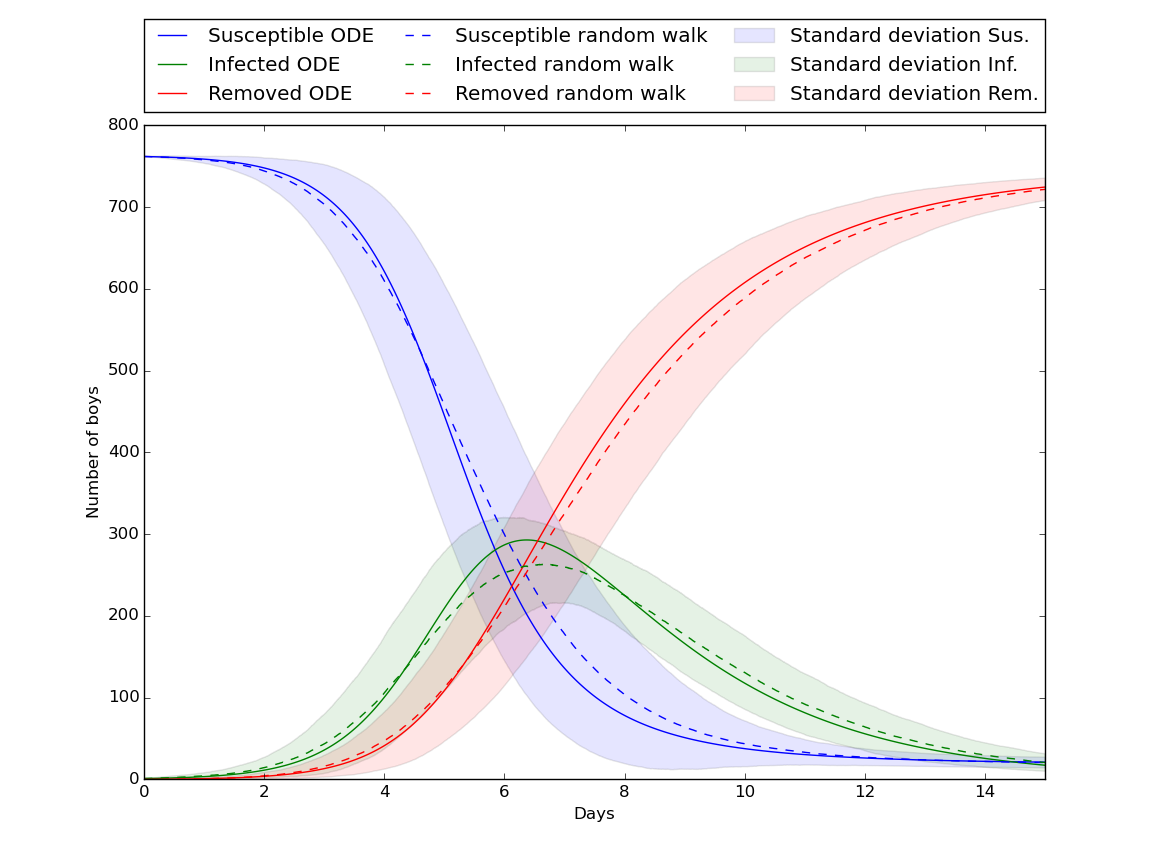
\includegraphics[width=0.8\linewidth]{3_fig/english_school_random.png}}
  \caption{
  \label{fig:english_school_random}Random walk compared to an ODE simulation of Eq.(\ref{eq:SIR_model_random}. The random function is shown with a dashed line, with the standard deviation shown as the colored area around the dashed line. The random function is based on the average of a series of simulations.
  }
\end{figure}
%\clearpage % flush figures fig:english_school_random


\subsection{Lower maximum concentration for the \emph{Infected} group}
In the previous chapters, the threshold value was found for the epidemic systems. The reproduction rate could be used to check if the disease would develop into an epidemic disease. The reproduction rate can be seen in Eq.(\ref{eq:rep_rate})
\begin{equation} \label{eq:rep_rate}
R_0 = \frac{rS_0}{a}
\end{equation}
If $R_0> 1$ was fulfilled, an epidemic situation would occur. With the parameters from the ODE simulation, he result would be $R_0 = 3.77$. This information could be used to find the maximum concentration of the \emph{Infected} group. This was shown in Section~\ref{section:1threshold_phenomenon} in Chapter~\ref{section:ODE_models}. In the two previous chapters, the maximum value of \emph{Infected}, given by $I_{max}$ has been set to 292.8. By studying the Fig.(\ref{fig:english_school_random}), one can see that the maximum value of the random walk simulation is lower, and occur later. The maximum value of the \emph{Infected} group is here measured to be 263.2. 


\vspace{3mm}




\vspace{3mm}


Since the transformation of a student from the \emph{Susceptible} group to the \emph{Infected} group only requires one successful meeting, where successful is seen as the transmission of the disease. There will be no difference in the result if the transmission of the disease happens once or several times during one time step. However, if the number of \emph{Infected} increases, the risk of one person getting infected several times increases as well. If a person gets infected, the incubation time will be set and not vary related to the amount of sick ones around. Based on a report from Centers for Disease Control and Prevention from 2008, the incubation time for influenza is between 1 and 4 days, and the average is 2 days. None of these models takes the incubation time into account. However, the way of getting infected differs between the models. This result in a difference in $\Imax$ 
% http://www.cdc.gov/flu/professionals/acip/clinical.htm

\subsection{The chance for a disease to spread}
When calculating the group of simulations, only 75 percent of the simulations resulted in an epidemic disease. 25 percent resulted in a transmission of the infected student to the \emph{Removed} group, before the student was able to infect other students. These simulations were performed on a small group, and the results may differ in larger groups. A removal rate above one will not necessarily lead to an epidemic disease, if the group is small enough.

% max inf 263.186666667


\section{Zombiefication}
The ODE system given in the chapter \emph{ODE models} will be used for this simulation. This can be seen in Eq.(\ref{eq:seland_model_random}). The parameters have to be adjusted for this simulation, similarly to the parameters for English boarding school. Frederikkeplassen at Blindern will be used as the area where the simulations will be done. The area is estimated to be 100m x 100m and the disease will be able to spread if the distance is closer than 4 meters. There will be done four different simulations in this section, where the influence from human behavior to the model will be studied. The time unit will be set to minutes, and the simulations will be done for 10 minutes for the two first simulations. The last simulations will be performed for 34 minutes. 100 random steps will be performed every minute.       
\begin{equation} \label{eq:seland_model_random}
    \begin{aligned} 
    \frac{dS}{dt} =& \Sigma -(\beta+\mu \omega(t))SZ - \delta_SS \\
    \frac{dI}{dt} =& (\beta+\mu \omega(t))SZ - \varrho I - \delta_II\\
    \frac{dZ}{dt} =& \varrho I- (\alpha+\omega(t))SZ + \zeta R\\
    \frac{dR}{dt} =& \delta_SS +\delta_II -\zeta R + (\alpha+\omega(t))SZ 
    \end{aligned}
\end{equation}

Similarly to the English boarding school, the parameters in Eq.(\ref{eq:seland_model_random}) have to be adjusted. The parameters from the two first phases in \emph{Walking Dead} will be used. These can be seen in the table below. The number of meetings per minute is set to $m_0 = 98.64$, based on the average from 300 time steps. This is used to find the value of $\beta_r$ and $\alpha_r$, similar to the method shown in the previous section. The value for $\varrho$ has been adjusted by first finding the average incubation time for the \emph{Infected} group. This has been done by setting $1/\varrho$. The average incubation time is 0.72 minutes. This is really fast, and not a realistic number, based on the TV Series \emph{Walking Dead}. By numerical simulations, the value of $\varrho_r$ can be set to 0.0137 for each simulation. This will result in an average incubation time of 0.72 minutes. The same can be done for the value in the hysterical phase.  

\label{table:param_val_random}

\begin{quote}
\begin{tabular}{ccc}
\hline
\multicolumn{1}{c}{ parameter } & \multicolumn{1}{c}{ Initial phase } & \multicolumn{1}{c}{ hysterical phase } \\
\hline
$\beta$     & 0.01155       & 0.000011         \\
$\beta_r$   & 0.07271       & 0.000693         \\
$\varrho$   & 1.37          & 1.5              \\
$\varrho_r$ & 0.0137        & 0.015            \\
$\alpha$    & 0.00044       & 0.000208         \\
$\alpha_r$  & 0.00277       & 0.001309         \\
\hline
\end{tabular}
\end{quote}

\noindent
These parameter values are used for all simulations. The previous chapter \emph{Geographic models} introduced the spatial effect and the ability for humans to seek safe areas. This chapter will introduce different conditions for the walkers. These conditions will affect the interaction between the groups. In chapter \emph{ODE models}, the simulated period was estimated to 34 days. This will be different in this chapter. The section \emph{Ten minutes at Frederikkeplassen} in the previous chapter will be used as preference for the results. 

\subsection{Random walk}
Random walk will be the first condition for each walker. This results in a smooth distribution of the whole group. The simulation will be done for ten minutes at Frederikkeplassen. The simulations are shown with the python package <Pygame>, where the random walkers are represented with different images. These can be seen in Fig.(\ref{fig:figure_images}).


\begin{figure}[ht]
  \centerline{
\includegraphics[width=0.8\linewidth]{3_fig/figure_images.png}}
  \caption{
  \label{fig:figure_images} Figures used in the simulation. All seen from the sky. I: The walkers in the \emph{Susceptible} group can be seen as humans with green sweater. II: The walkers in the \emph{Infected} group can be seen with a red and green sweater, with one arm in front. III: The walkers in the \emph{Zombie} group can be seen with a white sweater and both arms in front. IV: the walkers in the \emph{Removed} group can be seen as a tombstone.
  }
\end{figure}
%\clearpage % flush figures fig:figure_images


The initial values for the four groups are similar as in the previous chapter. $S_0 = 621$, $I_0 = 0$, $Z_0 = 1$ and $R_0 = 0$. The walkers are randomly distributed over Frederikkeplassen at initial time. The initial positions in one simulation can be seen in subplot I in Fig.(\ref{fig:initial_final}).The probability distribution function for the walkers are here set to be uniform. The walkers will therefore have the same probability for walking in all directions. The step length is based on an average pace of 5 kilometers per hour. This result in a step length of 0.83 m for each random walk. The first simulation is run for 10 minutes. The parameters from the \emph{Initial phase} are used from 0 to 3 minutes. From 3 to 10 minutes, the parameters from the \emph{Hysterical phase} are used. The result after 10 minutes can be seen in subplot II in Fig.(\ref{fig:initial_final}). 


\begin{figure}[ht]
  \centerline{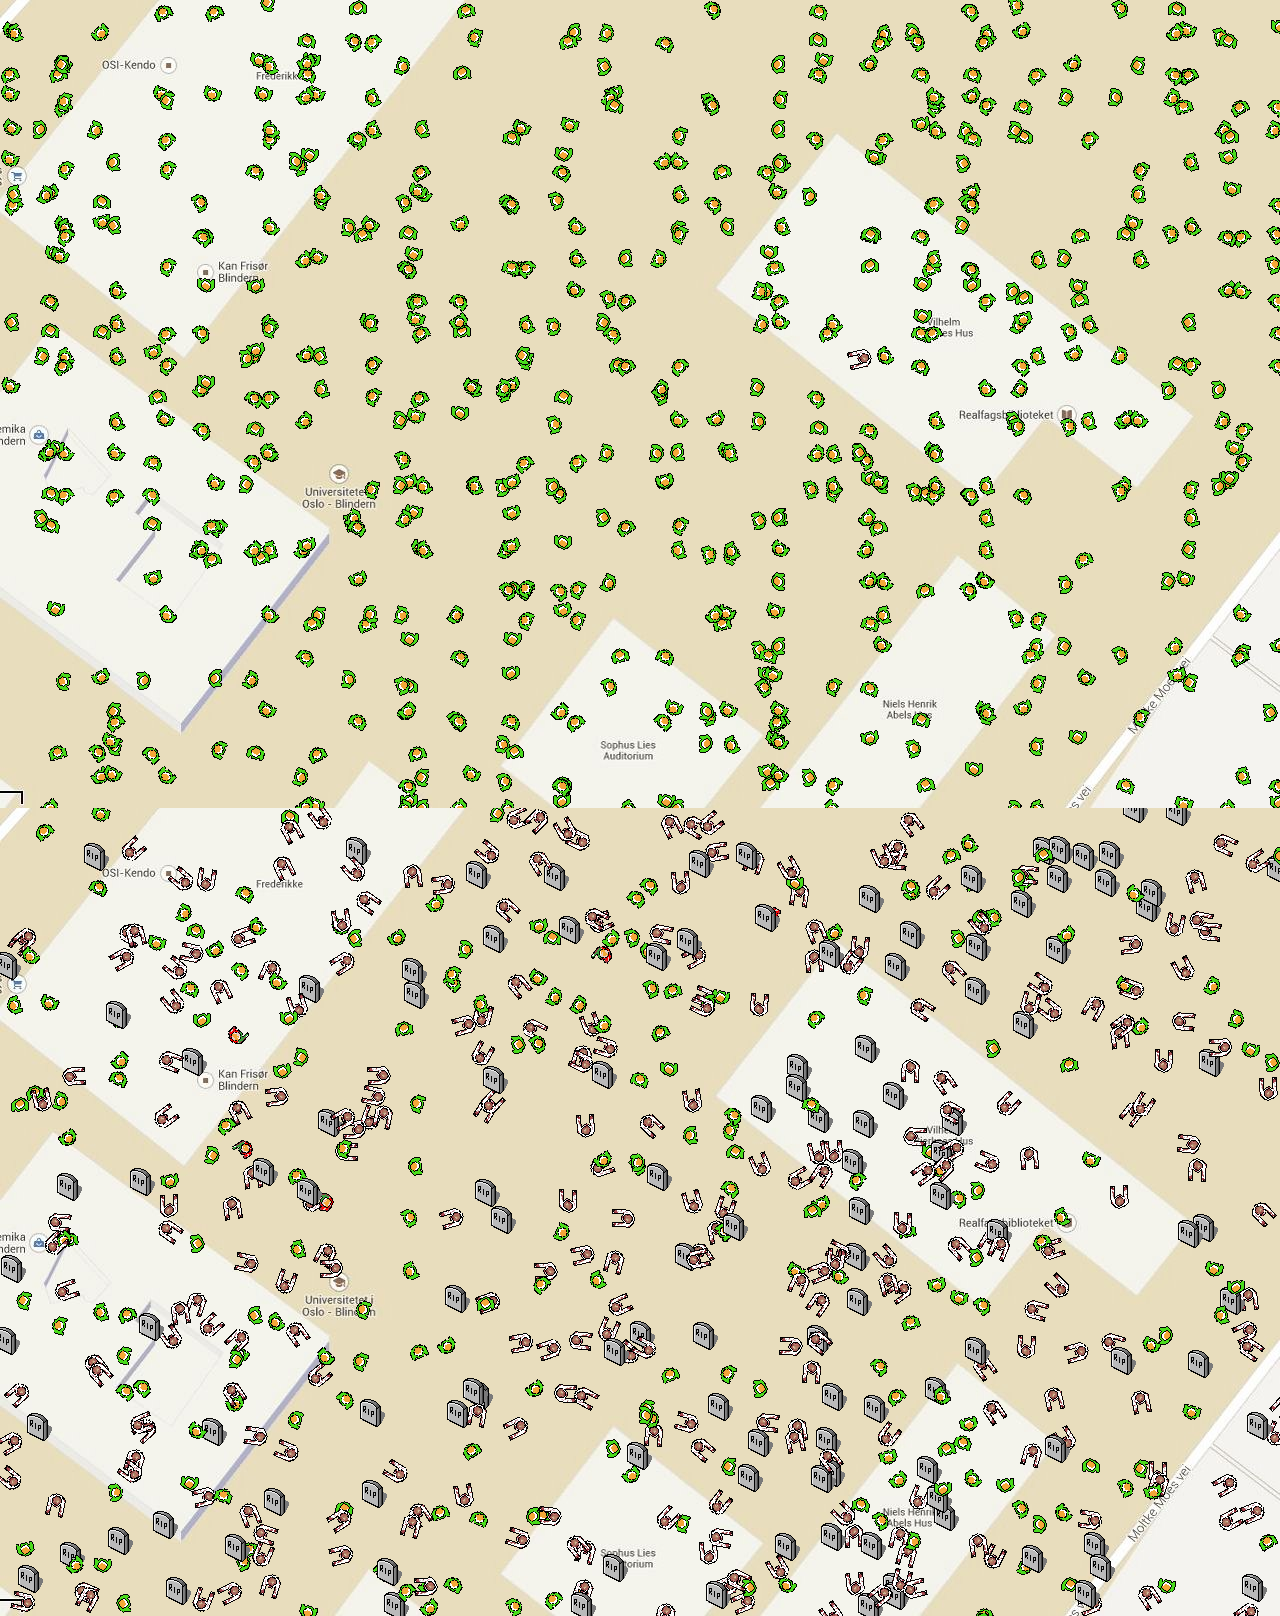
\includegraphics[width=0.8\linewidth]{3_fig/Frederikke_initial_final.png}}
  \caption{
  \label{fig:initial_final} Positions from the simulations of Frederikkeplassen. I: Initial position for 621 susceptible humans and 1 zombie. II: Final position of a simulation of Frederikkeplassen.
  }
\end{figure}
%\clearpage % flush figures fig:initial_final


100 simulations with these parameter values are performed, and the average and standard deviation of the simulations are plotted in Fig(\ref{fig:walking_dead}). 95 percent of the simulations led to an epidemic disease. However, the standard deviation is large. By studying the second phase from 3 minutes to 10 minutes, one can see that the amount in each group varies. In the \emph{Hysterical phase}, the standard deviation is high for the \emph{Susceptible} and \emph{Zombie} groups. Therefore the outcome from a random chosen simulation is hard to predict.


\begin{figure}[ht]
  \centerline{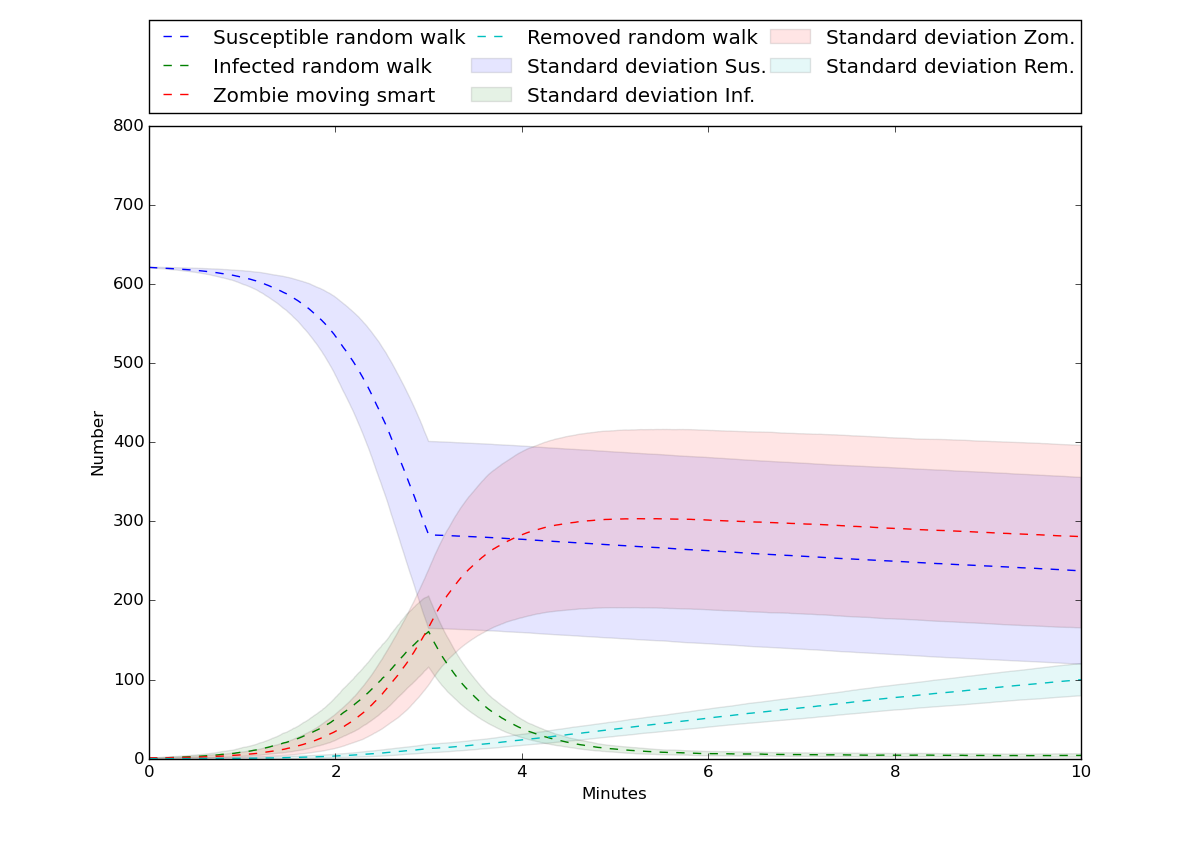
\includegraphics[width=0.8\linewidth]{3_fig/Walking_dead_Frederikke.png}}
  \caption{
  \label{fig:walking_dead}The average and standard deviation of 190 simulations on Frederikkeplassen. The \emph{Initial phase} lasts from 0 to 3 minutes.The \emph{Hysterical phase} lasts from 3 to 10 minutes. The parameter values can be seen in Tab.(\ref{table:param_val_random}).
  }
\end{figure}
%\clearpage % flush figures fig:walking_dead


By comparing the average result with the PDE simulation from \emph{Ten minutes at Frederikkeplassen} in the previous chapter, one can see that the average results differ from the PDE results. The average number of the \emph{Susceptible} group is higher than the result from the PDE simulation. 

\label{table:frederikke_table_random}

\begin{quote}
\begin{tabular}{cccc}
\hline
\multicolumn{1}{c}{  } & \multicolumn{1}{c}{ PDE } & \multicolumn{1}{c}{ Random walk } & \multicolumn{1}{c}{ Moving smart } \\
\hline
3 Minutes   & ----------- & ------------ & ------------ \\
\hline
Susceptible & 72.23       & 279.2        & 87.51        \\
Infected    & 229.65      & 162.05       & 229.02       \\
Zombie      & 296.67      & 167.57       & 284.88       \\
Removed     & 20.84       & 13.168       & 20.59        \\
\hline
7 Minutes   & ----------- & ------------ & ------------ \\
\hline
Susceptible & 70.78       & 276.36       & 82.79        \\
Infected    & 0.83        & 0.6421       & 35.35        \\
Zombie      & 498.72      & 278.87       & 397.46       \\
Removed     & 49.12       & 66.115       & 106.4        \\
\hline
10 Minutes  & ----------- & ------------ & ------------ \\
\hline
Susceptible & 69.69       & 274.34       & 79.96        \\
Infected    & 0.25        & 0.4736       & 34.87        \\
Zombie      & 479.00      & 243.48       & 350.15       \\
Removed     & 70.55       & 103.69       & 157.02       \\
\hline
\end{tabular}
\end{quote}

\noindent



\subsection{Moving smart}
Next phase is based on the movement pattern that would be more realistic based on the TV series \emph{Walking Dead}. Here the \emph{Zombie} group searches after humans from the \emph{Susceptible} group in the area around them. If there are humans that are close enough, the zombies will start moving towards the humans. The same is done for the humans in the \emph{Susceptible} group. The humans search after possible attacks from the zombies. When the zombies get to close, the humans try to escape by moving away. If the distance between the zombie and human is to high, they will randomly walk around. 


\vspace{3mm}




\vspace{3mm}


Similar to the random walk condition above, the moving smart condition is calculated based on 100 simulations. The step length is equal for the \emph{Susceptible} group and the \emph{Zombie} group. Therefore the number of zombies are set to 10, to avoid a chasing game, where one zombie runs after the group of \emph{Susceptible} with the equal distance the whole time. A screenshot of one simulation can be seen in Fig.(\ref{fig:screenshot_moving_smart}). One can see that the zombies chase the humans around. The zombies have to cooperate to be able to get close enough to attack the humans.  


\vspace{3mm}




\vspace{3mm}




\begin{figure}[ht]
  \centerline{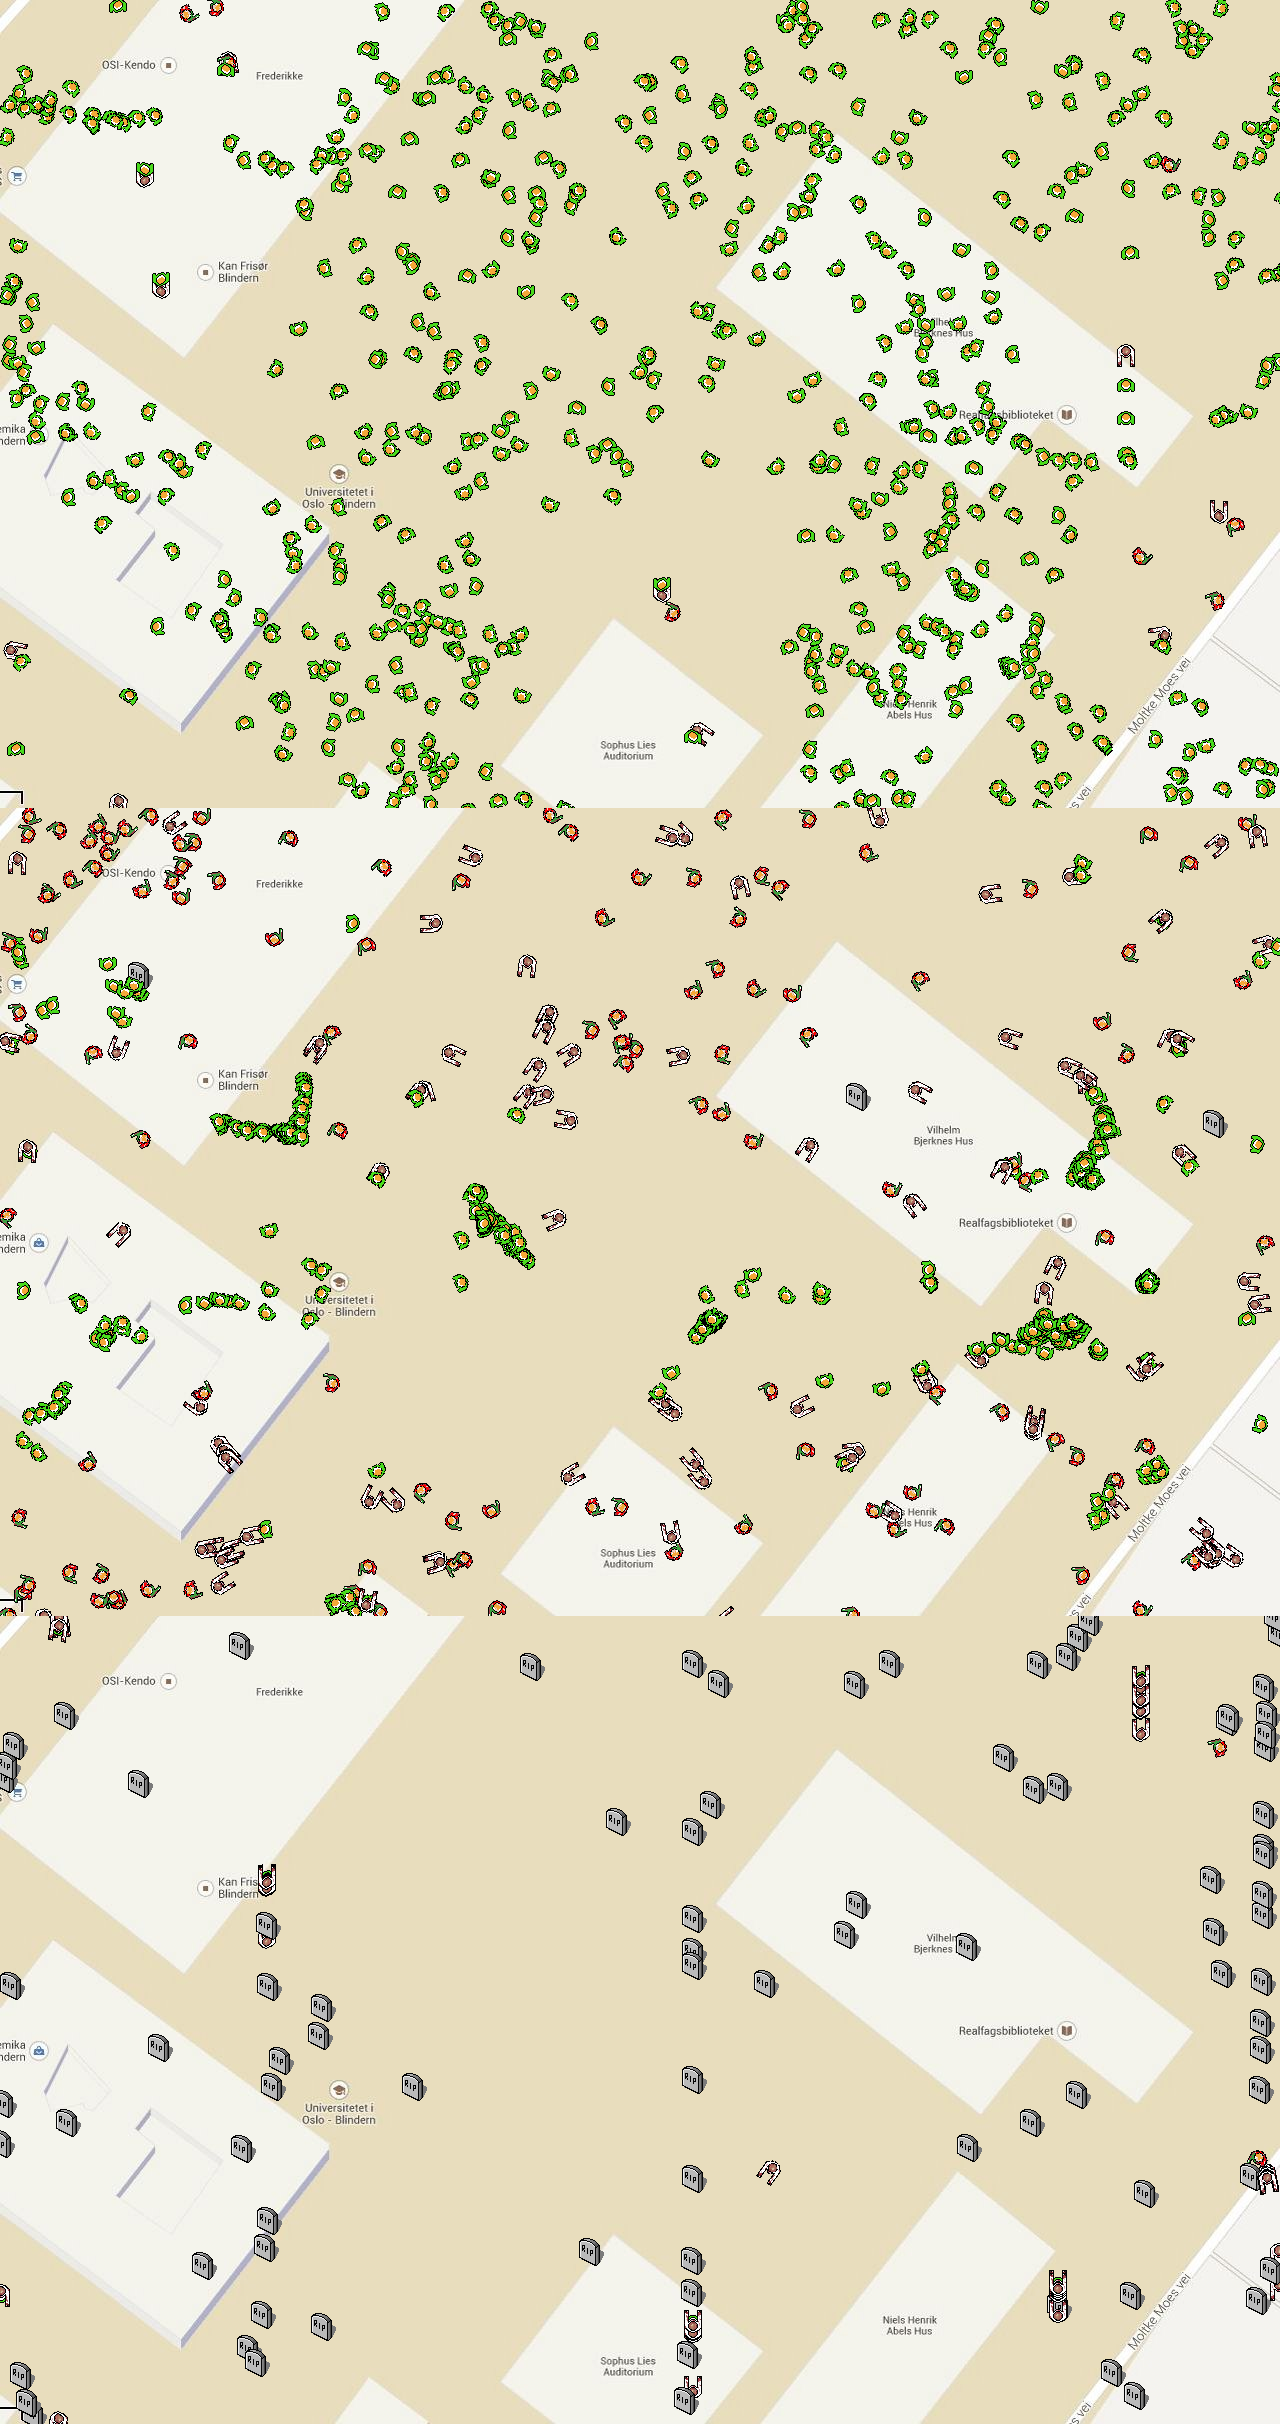
\includegraphics[width=0.8\linewidth]{3_fig/screenshots_moving_smart.png}}
  \caption{
  \label{fig:screenshot_moving_smart} Three Screenshots of the moving pattern for the \emph{Zombie} and \emph{Susceptible} group with the moving smart condition.I:Close after initial time. The zombies are chasing the humans.II: A large group of humans have recently been infected in the upper left corner. III: Close to total eradication for the human group. Only a small group left in the center of Frederikke.
  }
\end{figure}
%\clearpage % flush figures fig:screenshot_moving_smart


Some simulations were first tried where only one zombie was initialized at the start. This resulted in zero infected humans and a chasing zombie as explained above. However, when the amount of zombies was increased to 10, the difference in the result was major. One can see in Tab.(\ref{table:frederikke_table_random}) that after the \emph{Initial phase}, there are only 100 susceptible humans left in the average moving smart. The cooperating force from the \emph{Zombie} group gets stronger as the group increases. Then they are able to chase the \emph{Susceptible} group from several fronts, and it is difficult for the \emph{Susceptible} group to avoid fights. Similar situations are seen in \emph{Walking Dead}. In the city Atlanta, where the amount of zombies is high, the ability to escape is difficult. However, when the main character Rick Grimes meets individual zombies, he can easily escape the danger. A plot of the average result with the standard deviation can be seen in Fig.(\ref{fig:average_moving_smart}). 


\vspace{3mm}




\vspace{3mm}




\begin{figure}[ht]
  \centerline{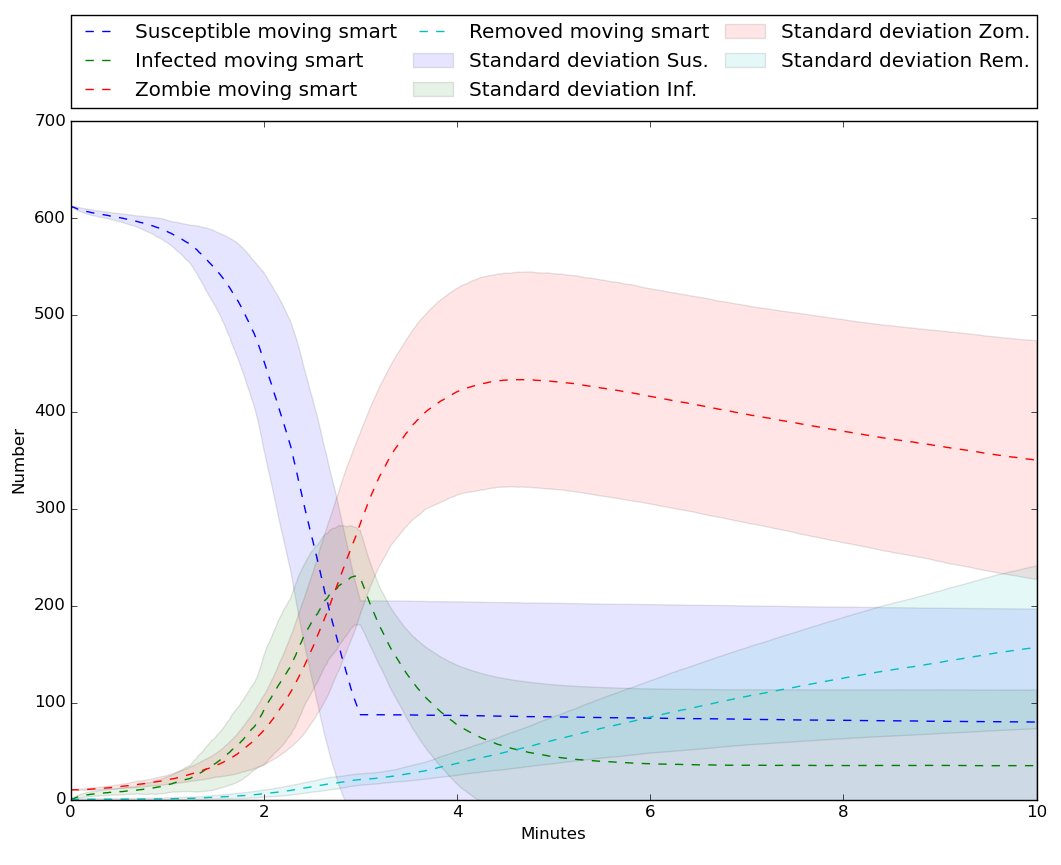
\includegraphics[width=0.8\linewidth]{3_fig/Moving_smart_average.png}}
  \caption{
  \label{fig:average_moving_smart} The average and standard deviation of for the moving smart conditionon Frederikkeplassen. The \emph{Initial phase} lasts from 0 to 3 minutes.The \emph{Hysterical phase} lasts from 3 to 10 minutes. The parameter values can be seen in Tab.(\ref{table:param_val_random}).
  }
\end{figure}
%\clearpage % flush figures fig:average_moving_smart


A result of this cooperating force from the \emph{Zombie} group is that the group is able to eradicate the \emph{Susceptible} group in several simulations. After the \emph{Initial phase}, 15 of the 100 simulations results in total eradication for the \emph{Susceptible} group. At final time the number of simulations that causes eradication have increased to 29 simulations. This moving smart condition seems to give the \emph{Zombie} group the greatest advantage, when the density of zombies gets high.

\subsection{Three phases in Walking Dead}
A natural idea is to use different conditions for different phases. The first phase, \emph{Initial phase}, will include a random walk condition for all groups. While the \emph{Hysterical phase} will include a smart moving condition for the \emph{Susceptible} and \emph{Zombie} group. The \emph{Infected} group will move randomly around as in the \emph{Initial phase}. The third phase will be the \emph{Counter attack}, where the \emph{Susceptible} group will stop running and then counter attack the zombies. The strength of the attack depends on the density of humans around. If the density of humans is high in an area, the strength of the \emph{Susceptible} group will increase. This is not the case for the \emph{Zombie} group. The simulation will be performed for 34 minutes, where the three phases have been scaled down from days to minutes. This simulation will not be able to say anything about the result for 34 days. This will demand other values. This result will give an insight into how human behavior will affect the result.  


\vspace{3mm}




\vspace{3mm}


The \emph{Susceptible} group will at initial time be split into three groups. The distribution in the groups will be based on a Gaussian distribution explained section~\ref{sec:monte_carlo_methods}. The \emph{Susceptible} groups are placed at the following positions: 21 humans at position(6,6), 200 humans at position(12,25) and 400 humans at (25,12). The initial position for the zombie is randomly placed around for all simulations. 100 simulations are performed. Screenshots from a simulation can be seen in Fig.(\ref{fig:screenshots_three_phases}). 


\vspace{3mm}




\vspace{3mm}




\begin{figure}[ht]
  \centerline{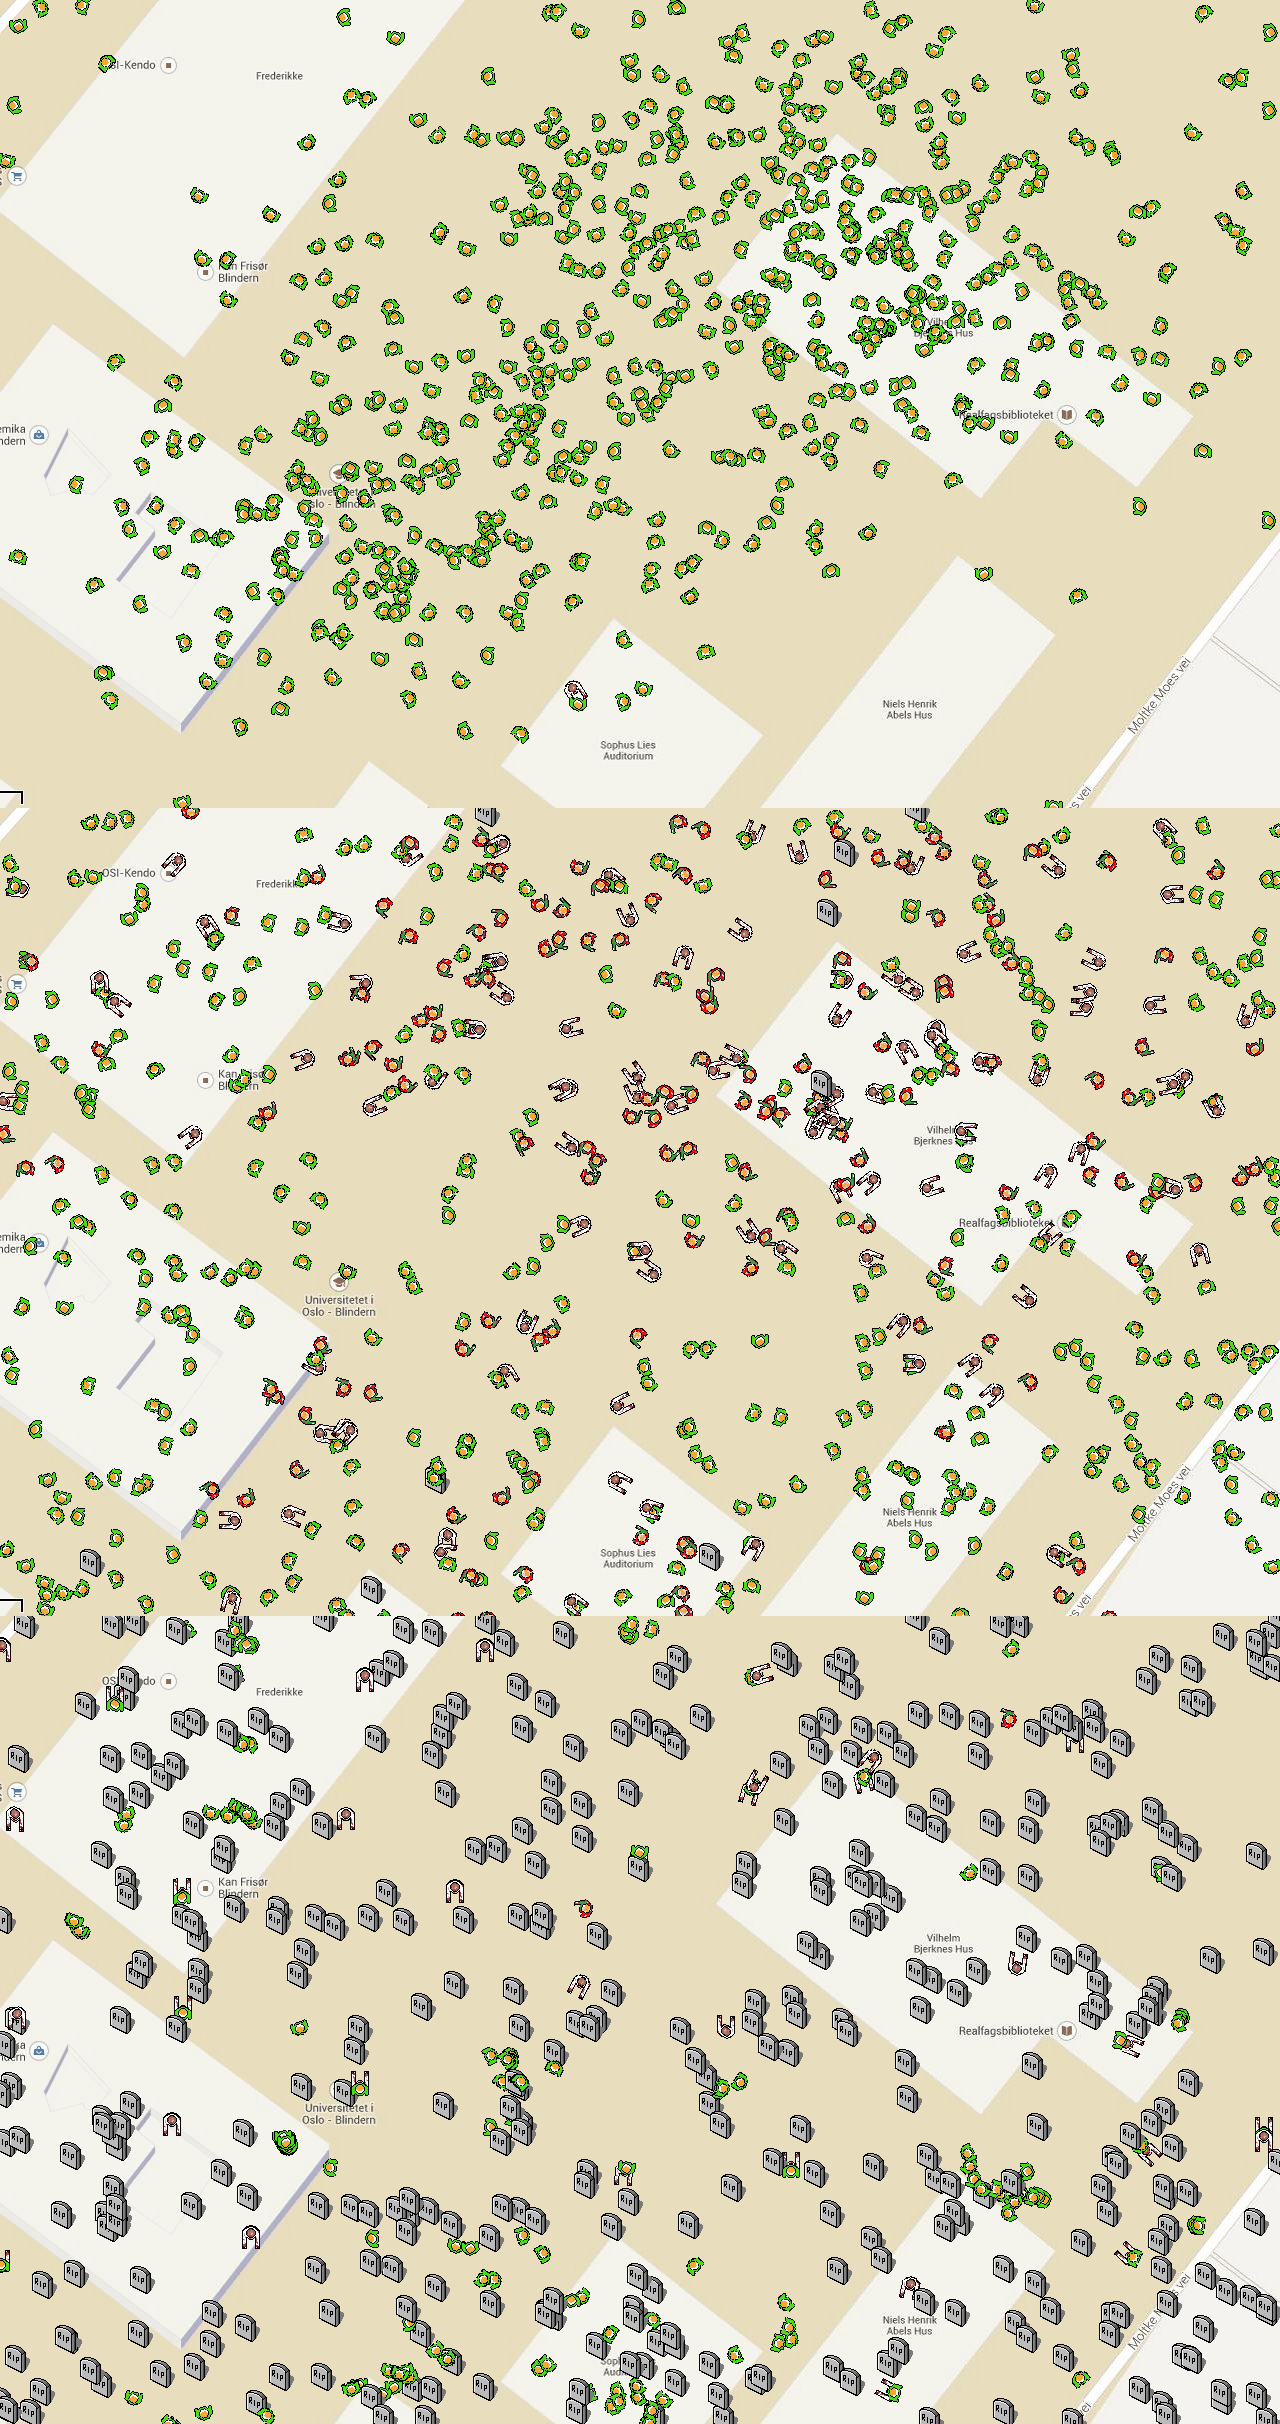
\includegraphics[width=0.8\linewidth]{3_fig/three_phases_random.png}}
  \caption{
  \label{fig:screenshots_three_phases} Three screenshots from a simulation of the three phases. I: Shows the initial position of the \emph{Susceptible} and \emph{Zombie} group. II: Shows the position and number before the \emph{Hysterical phase}. III: shows the result after the \emph{Hysterical phase}.
  }
\end{figure}
%\clearpage % flush figures fig:screenshots_three_phases





\begin{figure}[ht]
  \centerline{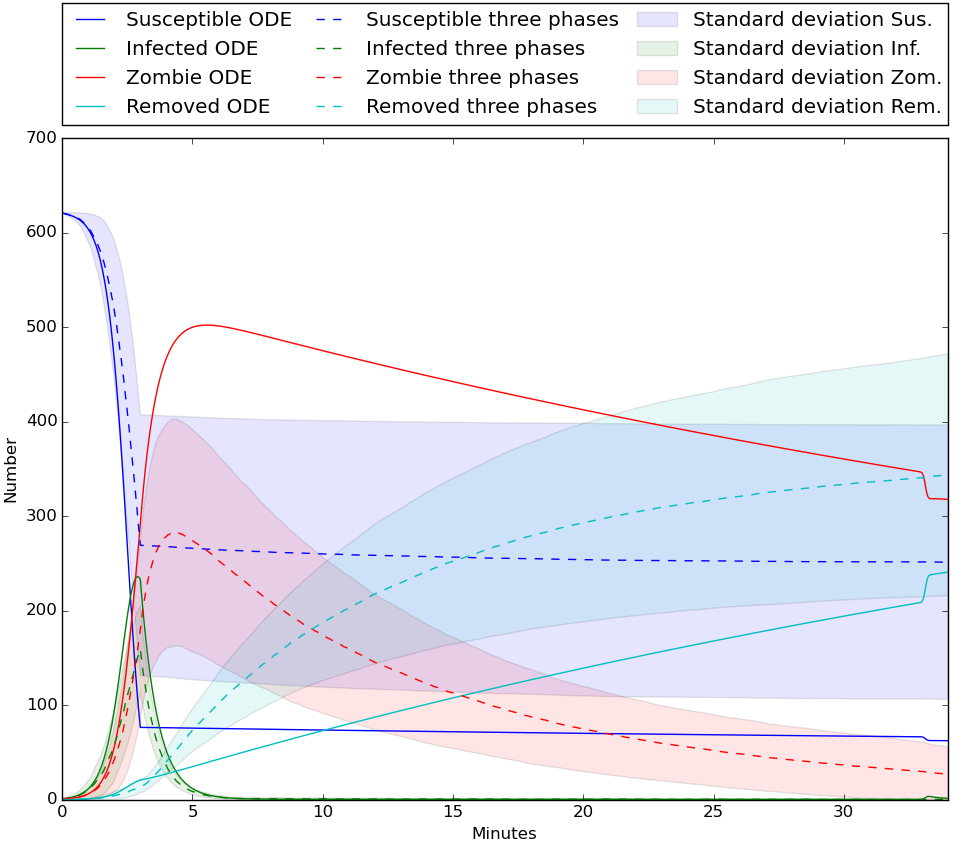
\includegraphics[width=0.8\linewidth]{3_fig/three_phases_ODE_sd.png}}
  \caption{
  The average and standard deviation for a set of simulations over three phases. An ODE simulation withthe same parameters is added to the plot.
  }
\end{figure}
%\clearpage % flush figures 


% Data: 187 success
% Eradication 3:0
% Eradication 33:0
% Eradication 34:0

By studying the Tab.(\ref{table:compare_ODE_random}), the three phases gives the \emph{Susceptible} group a greater chance of staying alive. One can see that there is only 1 person from the \emph{Susceptible} group that dies in the Hysterical phase compared to 4 in the ODE simulation. The similar result can be seen for the \emph{Zombie} group. There are several that dies in the ODE simulation that in the Random walk simulation. This can be explained by the fact that the \emph{Susceptible} group tries to avoid fights by running away. 

\label{table:compare_ODE_random}

\begin{quote}
\begin{tabular}{cccc}
\hline
\multicolumn{1}{c}{  } & \multicolumn{1}{c}{ ODE } & \multicolumn{1}{c}{ Random walk } & \multicolumn{1}{c}{ Free areas } \\
\hline
Initial phase    & -------- & ------------ & ----------- \\
\hline
Susceptible      & 71       & 274          & 328         \\
Infected         & 231      & 157          & 131         \\
Zombie           & 299      & 178          & 151         \\
Removed          & 21       & 14           & 12          \\
\hline
Hysterical phase & -------- & ------------ & ----------- \\
\hline
Susceptible      & 62       & 256          & 326         \\
Infected         & 0        & 0            & 0           \\
Zombie           & 359      & 31           & 259         \\
Removed          & 202      & 335          & 37          \\
\hline
Counter attack   & -------- & ------------ & ----------- \\
\hline
Susceptible      & 58       & 256          & 326         \\
Infected         & 1        & 0            & 0           \\
Zombie           & 332      & 28           & 258         \\
Removed          & 231      & 338          & 37          \\
\hline
\end{tabular}
\end{quote}

\noindent




\subsection{Free areas for the \emph{Susceptible} group}
The last advantage the \emph{Susceptible} group will get, is to be able to move into buildings to escape the zombies. A similar thing was done for in the previous chapter, \emph{PDE models}. However, the effect is better here. The free areas are found by using the pixel values for the backgroud picture. The value of the buildings is similar for all buildings, and is used to control the direction of the \emph{Zombie} group. Nothing is done for the \emph{Susceptible} group. The movement pattern for the susceptible students will only be affected by the positions of the zombies. A screenshot after 10 minutes can be seen in Fig.(\ref{fig:screenshot_three_phases_free})


\vspace{3mm}




\vspace{3mm}




\begin{figure}[ht]
  \centerline{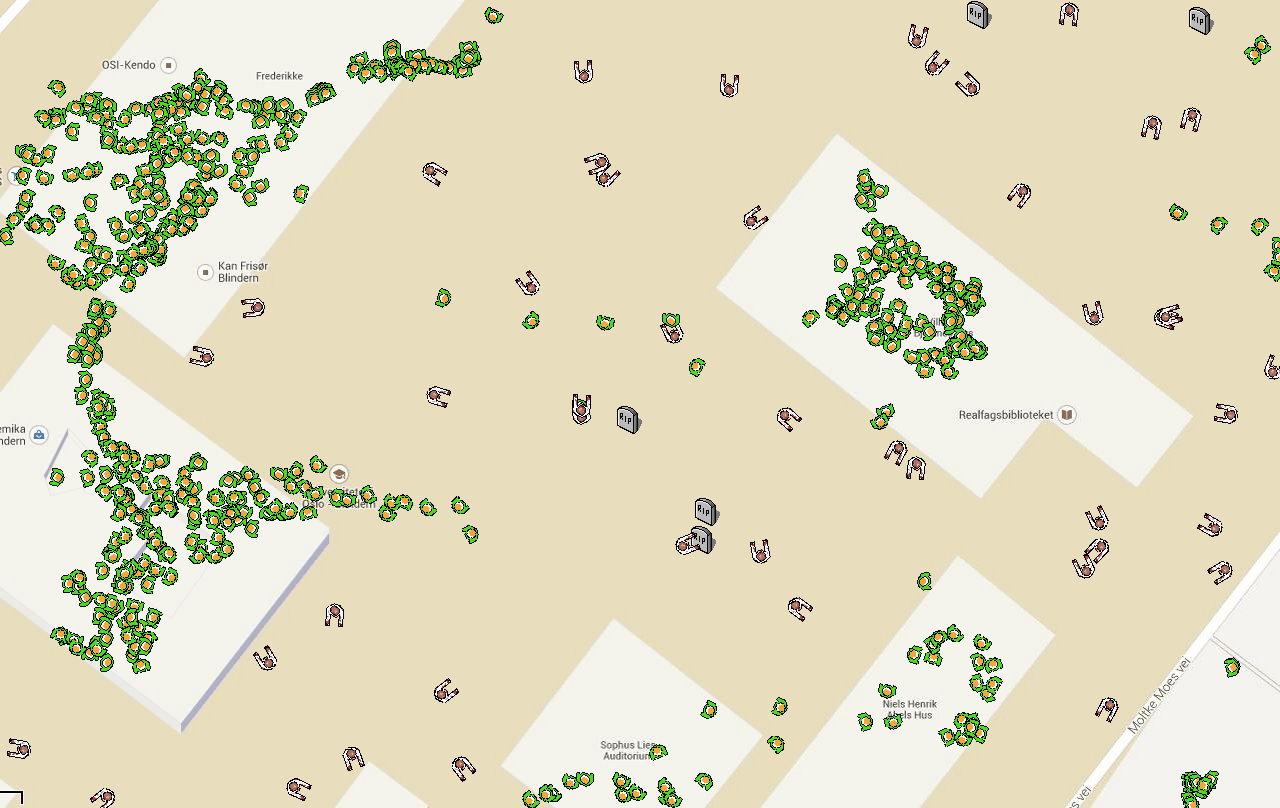
\includegraphics[width=0.8\linewidth]{3_fig/screenshot_three_phases_free.png}}
  \caption{
  \label{fig:screenshot_three_phases_free} A screenshot of a simulation over three phases with free areas for the \emph{Susceptible} group inside the buildings. The scrennshot is taken 10 minutes into the simulation. In the \emph{Hysterical phase}.
  }
\end{figure}
%\clearpage % flush figures fig:screenshot_three_phases_free


One can see from Fig.(\ref{fig:screenshot_three_phases_free}) that the humans moves into the buildings. These are not defined as any free areas. However, the zombies are not able to go in here, and the result is that this becomes the desired area for the humans. By studying Fig.(\ref{fig:three_phases_free}), one can see that the change in amount of zombies and humans flattens out over time, this can be explained by the fact that the humans are now able to avoid battles. The \emph{Counter attack} phase in negligible in the simulation with free areas. Since the humans are able to avoid connections with the zombies, the counter attack disappears.  


\begin{figure}[ht]
  \centerline{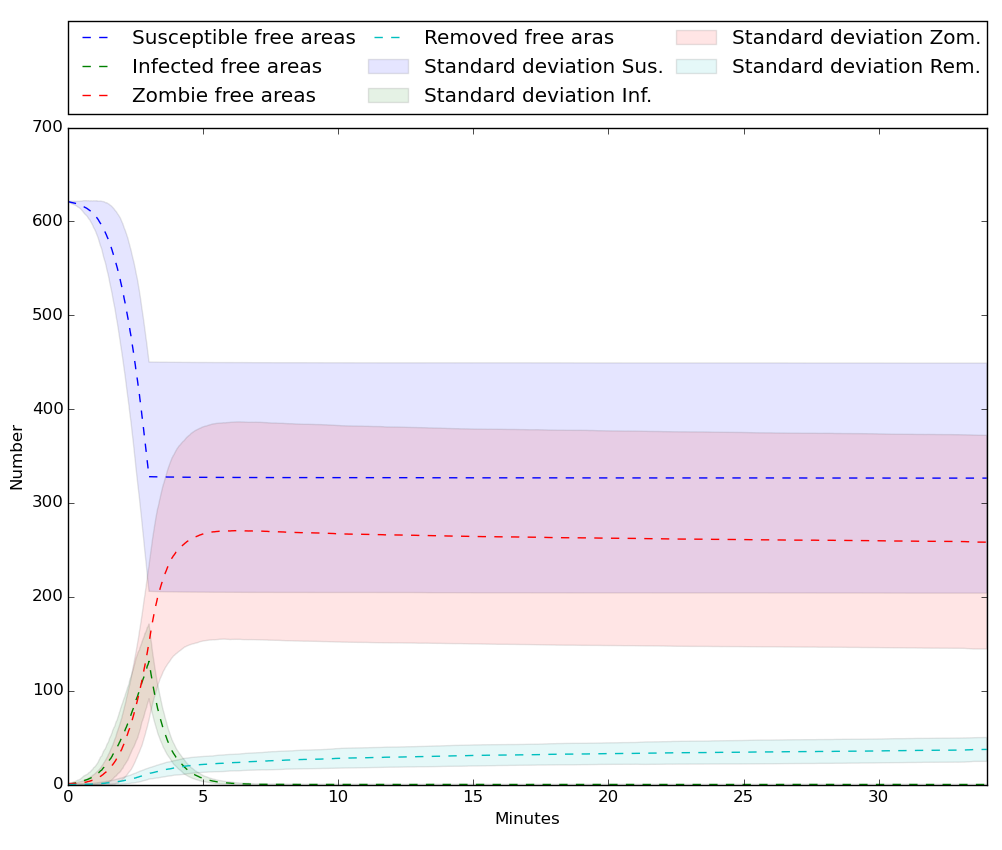
\includegraphics[width=0.8\linewidth]{3_fig/three_phases_free.png}}
  \caption{
  \label{fig:three_phases_free} The average and standard deviation for a set of simulations over three phases, with free areas inside the buildings. Initial values $S_0 = 621$, $I_0 = 0$, $Z_0=1$ and $R_0=0$.
  }
\end{figure}
%\clearpage % flush figures fig:three_phases_free






\section{Discussion}
The results from the English boarding school shows that the maximum concentration of the \emph{Infected} is reduced when using random walk to simulate the disease. The incubation time for influenza has one day as the shortest incubation time. The model used for the English boarding school is a SIR model, and the model skips this incubation phase. This is not the case for the random walk model. One time step is needed to transpose a student from the \emph{Susceptible} class to the \emph{Infected} class. 


\vspace{3mm}




\vspace{3mm}


Another result from the English boarding school was the number of successful epidemic simulations. 5 % of the simulations resulted in no epidemic situation. The infected student was transposed to the \emph{Removed} group before he was able to infect other students. When modelling closed systems, especially with a small group, the chance of an epidemic situation to occur is lower than for a larger group.  


\vspace{3mm}




\vspace{3mm}


The zombiefication part for this chapter was only modeled for minutes. The idea was to study the effect of human behavior. The average result from the random walk simulations in Fig.(\ref{fig:walking_dead}) showed a large standard deviation for the groups. It is therefore difficult to predict the result. The similar situation was for the other condition moving smart. This condition was first given to improve the humans ability to survive. With a small group of zombies, this was the case. However, when the group of zombies increased the cooperation force become strong. These simulations were performed on a small area which gave the zombies an advantage. It was then easier for the \emph{Zombie} group to surround the \emph{Susceptible} group. This lead to eradication of the \emph{Susceptible} group in several of the simulations.


\vspace{3mm}




\vspace{3mm}


The two lasts sections consists of simulations of all three phases from \emph{Walking Dead}. These are modeled for a shorter time than the series. However, these simulations gives some interesting results. The first simulation of the three phases tries to add the movement pattern that is realistic based on the series \emph{Walking Dead}. This result in the ability to avoid battles, and the loss of \emph{Susceptible} is reduced. An interesting study further, would be if the moving smart phase could compensate for the changes in parameter values in each phase. The idea by changing the parameter values in the ODE and PDE systems, is to illustrate changes in the behavior. The last simulation add the free areas for the \emph{Susceptible} group. A similar thing was done for the PDE system in the previous chapter. However, the expected result was easier achieved in this simulation. It is interesting to see that the preferred area for the humans was the buildings. The \emph{Susceptible} group had no knowledge about the safety in the buildings, only a desire to avoid the zombies. 


\chapter{Discussion and conclusion}
This paper has used three different systems to model epidemic diseases. These three models gives different possibilities related to the adaptation to real epidemic situations. The first chapter \emph{ODE systems}, models the changes in different groups based on the time aspect. This does not take into account the spatial distribution and is easy to use if a model should be adapted to a already given result, or if the simulation is done for a large, uniform group. The three phases in \emph{Walking Dead} were modeled by adjusting the parameter values to fulfill the expected amount for each group. The model is good to use in the result is known. However, since the spatial factor plays a major role in how a disease spred, this model will not take this information into account. 


\vspace{3mm}




\vspace{3mm}


The chapter \emph{PDE models} added the spatial factor. From the English boarding school, one could see that the position of the infected student had a major impact on the result. This was expanded for the \emph{Zombiefication} model, where the \emph{Susceptible} group was spread. One could see that the positions for the groups was important. This chapter also introduce \emph{Ten minutes at Frederikke}, where the idea is to add human behavior to the model. The diffusion term gave restrictions for the areas where the zombies could move, which resulted i a higher amount of humans that survived. This idea did not work that good, since the concentrations in a PDE system wants fullfil equilibirum. 


\vspace{3mm}




\vspace{3mm}


Random walk gave the opportunity to add human behavior in an easier way. Since the random walk model is based on a set of choises that the random walker needs to do every time step, the expected behavoir can be implemented. Compared to \emph{Walking Dead}, the different conditions in the random walk model reflects the behavior from the humans and zombies in the series. The moving smart condition takes away some of the random walk aspect. However, it also adds a more realistic behavoir. By presenting the situation where a zombie outbust would happen, a random walk would not be a natural and realistic way to move. Neither for a larger group. 


\vspace{3mm}




\vspace{3mm}


The idea by adding areas where the zombies could not move, worked a lot better for the random walk model than the PDE model. The group that was simulated here, aws quite small and the result would may differ if the group was larger. The focus in this thesis has been on small groups the the ability to add human behavior. The random walk model was the one that gave the best results. However, it also demands most computational force.

\subsection{Further work}
It would be interesting to expand the random model by simulating for a longer time scale with a higher amount of people. The code in this thesis has been written i python,which results in a slow simulating. By paralellisizing the code and divide the different simulations into different areas, one could done a more qualified simulation of a zombie outburst.


\vspace{3mm}




\vspace{3mm}


The idea of adding more parameters to the random walker, would make it more realistic. The skills for a human was similar for all in the \emph{Susceptible} group. This is not the case in the real world. All humans have different skills and would behave different in meeting with a zombie. Interesting skills to add would be:
\begin{itemize}
\item weapons for the \emph{Susceptible} group

\item noise sensitive for the \emph{Zombie} group

\item The ability to cooperate
\end{itemize}

\noindent
This would all make the random walk model more realistic in the idea of simulating a zombie outburst.



\chapter{Appendix}


\subsection{Diffusion equation and random walks}
The British Botanist R. Brown developed a theory by studying how pollen dispersed in water. This idea is called Brownian motion and can be used to describe a group of particles spreading. The function $w(x,t)dx$ can be defined as the probability of finding a given number of particles in an interval with size $dx$. This function is the $PDF$ as explained in the section above. The flux of particles that passing a point $x$, can be described by $j(x,t)$. This flow is proportionally with the gradient of the $PDF$,
\begin{equation}
j(x,t) = -D\frac{\partial w(x,t)}{\partial x}
\end{equation}
$D$ is here the diffusion constant. This example can be seen as a closed experiment, where the concentration is conserved. The relation between the flux and the $PDF$ can also be expressed
\begin{equation}
\frac{\partial j(x,t)}{\partial x} = -\frac{\partial w(x,t)}{\partial t} 
\end{equation}
And a diffusion equation can be expressed based on these two equations.
\begin{equation}
\frac{\partial w(x,t)}{\partial t} = D\frac{\partial^2 w(x,t)}{\partial x^2} 
\end{equation}
The expectation value and the variance, $\sigma^2$, can be study. The expectation value for the function $f(x,t)$ can be defined as
\begin{equation}
\langle f(x,t) \rangle = \int^{\infty}_{-\infty} f(x,t) w(x,t)dx
\end{equation}
The demands defined for the PDF in the previous section have to be fulfilled for $w(x,t)$. The normalization condition which is defined for this PDF require constraints for equation.
\begin{equation} \label{eq:PDF_demands}
w(x= \pm \infty,t) = 0,\quad \frac{\partial^nw(x,t)}{\partial x^n}|_{x=\pm\infty} = 0 
\end{equation}
This can be used to study the time derivative of the expectation value. The diffusion equation derived earlier can be used here.
\begin{equation}
\frac{\partial \langle f(x,t) \rangle}{\partial t} = \int^{\infty}_{-\infty} f(x,t) \frac{\partial w(x,t)}{\partial t}dx = D \int^{\infty}_{-\infty} f(x,t) \frac{\partial^2 w(x,t)}{\partial x^2}dx
\end{equation}
By using integration by parts on the right side, the equation can be expressed,
\begin{equation} \label{eq:disp_0}
\frac{\partial \langle f(x,t) \rangle}{\partial t} = D f(x,t) \frac{\partial w(x,t)}{\partial x}|_{x=\pm \infty} - 2D \int^{\infty}_{-\infty} \frac{\partial w(x,t)}{\partial x}dx
\end{equation}
By using the demands from (\ref{eq:PDF_demands}), the $\langle f(x,t) \rangle$ is independent of time. 
\begin{equation}
\frac{\partial \langle f(x,t) \rangle}{\partial t} = 0
\end{equation}
Implying that if a simulation of a random walk with equal probability of jumping in each direction, will end up with the probability distribution centered around the initial position. This may not be the case for the variance. By using (\ref{eq:disp_0}), the $\langle x^2 \rangle $ can be found. 
\begin{equation} 
\frac{\partial \langle x^2 \rangle}{\partial t} = D x^2 \frac{\partial w(x,t)}{\partial x}|_{x=\pm \infty} - 2D \int^{\infty}_{-\infty} x\frac{\partial w(x,t)}{\partial x}dx
\end{equation}
Here, integration by parts can be used. This results in
\begin{equation}
\frac{\partial \langle x^2 \rangle}{\partial t} = D x w(x,t)|_{x=\pm \infty} + 2D \int^{\infty}_{-\infty} w(x,t)dx = 2D
\end{equation}
this leads to
\begin{equation}
\langle x^2 \rangle = 2Dt
\end{equation}
which gives the variance
\begin{equation} \label{eq:diff_var}
\langle x^2 \rangle -\langle x \rangle^2 = 2Dt
\end{equation}
And the square root of the variance can be expressed,
\begin{equation}
\sqrt{\langle x^2 \rangle -\langle x \rangle^2} = \sqrt{2Dt}
\end{equation}
By comparing this with the displacement of a free particle, which moves with the function $x(t)=vt$ from the initial point, will the diffusion process moves with $\sqrt{\langle x^2 \rangle -\langle x \rangle^2} \propto \sqrt{t}$. This can be used to describe a random walk, and could say that a random walker escapes much more slowly than a free particle from the initial time. This can be seen in an example. 



\clearemptydoublepage
\markboth{Bibliography}{Bibliography}
\thispagestyle{empty}

\bibliographystyle{plain}
\bibliography{../bibliography/papers}


% ------------------- end of main content ---------------


\clearemptydoublepage
\markboth{Index}{Index}
\thispagestyle{empty}
\printindex

\end{document}

